% Definizione di Prodotto
% da compilare con il comando pdflatex Definizione_di_prodotto_x.x.x.tex

% Dichiarazioni di ambiente e inclusione di pacchetti
% da usare tramite il comando % Dichiarazioni di ambiente e inclusione di pacchetti
% da usare tramite il comando % Dichiarazioni di ambiente e inclusione di pacchetti
% da usare tramite il comando \input{../../util/hx-ambiente}

\documentclass[a4paper,titlepage]{article}
\usepackage[T1]{fontenc}
\usepackage[utf8]{inputenc}
\usepackage[english,italian]{babel}
\usepackage{microtype}
\usepackage{lmodern}
\usepackage{underscore}
\usepackage{graphicx}
\usepackage{eurosym}
\usepackage{float}
\usepackage{fancyhdr}
\usepackage[table]{xcolor}
\usepackage{longtable}
\usepackage{chngpage}
\usepackage{grffile}
\usepackage[titles]{tocloft}
\usepackage{hyperref}
\hypersetup{hidelinks}

\usepackage{../../util/hx-vers}
\usepackage{../../util/hx-macro}
\usepackage{../../util/hx-front}

% solo se si vuole una nuova pagina ad ogni \section:
\usepackage{titlesec}
\newcommand{\sectionbreak}{\clearpage}

% stile di pagina:
\pagestyle{fancy}

% solo se si vuole eliminare l'indentazione ad ogni paragrafo:
\setlength{\parindent}{0pt}

% intestazione:
\lhead{\Large{\proj}}
\rhead{
\includegraphics[keepaspectratio=true,width=50px]{../../util/hivex_logo2.png}}
\renewcommand{\headrulewidth}{0.4pt}

% pie' di pagina:
\lfoot{\email}
\rfoot{\thepage}
\cfoot{}
\renewcommand{\footrulewidth}{0.4pt}

% spazio verticale tra le celle di una tabella:
\renewcommand{\arraystretch}{1.5}

% profondità di indicizzazione:
\setcounter{tocdepth}{4}
\setcounter{secnumdepth}{4}


\documentclass[a4paper,titlepage]{article}
\usepackage[T1]{fontenc}
\usepackage[utf8]{inputenc}
\usepackage[english,italian]{babel}
\usepackage{microtype}
\usepackage{lmodern}
\usepackage{underscore}
\usepackage{graphicx}
\usepackage{eurosym}
\usepackage{float}
\usepackage{fancyhdr}
\usepackage[table]{xcolor}
\usepackage{longtable}
\usepackage{chngpage}
\usepackage{grffile}
\usepackage[titles]{tocloft}
\usepackage{hyperref}
\hypersetup{hidelinks}

\usepackage{../../util/hx-vers}
\usepackage{../../util/hx-macro}
\usepackage{../../util/hx-front}

% solo se si vuole una nuova pagina ad ogni \section:
\usepackage{titlesec}
\newcommand{\sectionbreak}{\clearpage}

% stile di pagina:
\pagestyle{fancy}

% solo se si vuole eliminare l'indentazione ad ogni paragrafo:
\setlength{\parindent}{0pt}

% intestazione:
\lhead{\Large{\proj}}
\rhead{
\includegraphics[keepaspectratio=true,width=50px]{../../util/hivex_logo2.png}}
\renewcommand{\headrulewidth}{0.4pt}

% pie' di pagina:
\lfoot{\email}
\rfoot{\thepage}
\cfoot{}
\renewcommand{\footrulewidth}{0.4pt}

% spazio verticale tra le celle di una tabella:
\renewcommand{\arraystretch}{1.5}

% profondità di indicizzazione:
\setcounter{tocdepth}{4}
\setcounter{secnumdepth}{4}


\documentclass[a4paper,titlepage]{article}
\usepackage[T1]{fontenc}
\usepackage[utf8]{inputenc}
\usepackage[english,italian]{babel}
\usepackage{microtype}
\usepackage{lmodern}
\usepackage{underscore}
\usepackage{graphicx}
\usepackage{eurosym}
\usepackage{float}
\usepackage{fancyhdr}
\usepackage[table]{xcolor}
\usepackage{longtable}
\usepackage{chngpage}
\usepackage{grffile}
\usepackage[titles]{tocloft}
\usepackage{hyperref}
\hypersetup{hidelinks}

\usepackage{../../util/hx-vers}
\usepackage{../../util/hx-macro}
\usepackage{../../util/hx-front}

% solo se si vuole una nuova pagina ad ogni \section:
\usepackage{titlesec}
\newcommand{\sectionbreak}{\clearpage}

% stile di pagina:
\pagestyle{fancy}

% solo se si vuole eliminare l'indentazione ad ogni paragrafo:
\setlength{\parindent}{0pt}

% intestazione:
\lhead{\Large{\proj}}
\rhead{
\includegraphics[keepaspectratio=true,width=50px]{../../util/hivex_logo2.png}}
\renewcommand{\headrulewidth}{0.4pt}

% pie' di pagina:
\lfoot{\email}
\rfoot{\thepage}
\cfoot{}
\renewcommand{\footrulewidth}{0.4pt}

% spazio verticale tra le celle di una tabella:
\renewcommand{\arraystretch}{1.5}

% profondità di indicizzazione:
\setcounter{tocdepth}{4}
\setcounter{secnumdepth}{4}

\usepackage{placeins}

\version{2.0.0}
\creaz{28 febbraio 2017}
\author{\ALL}
\supervisor{\AZ, \PB}
\uso{interno}
\dest{\ALL}
\title{Definizione di Prodotto}

% Per neutralizzare \nogloxy eccetera:
\newcommand{\nogloxy}[1]{#1}
\newcommand{\subsubsubsection}[1]{\paragraph{#1}}
\newcommand{\textt}[1]{\texttt{#1}}

\begin{document}
\maketitle
% diario delle modifiche per il piano di progetto
% da includere con % diario delle modifiche per il piano di progetto
% da includere con % diario delle modifiche per il piano di progetto
% da includere con \include{diario}

\begin{diario}
	1.0.1 & {\GG} (Responsabile) & 03/02/2017 & Correzione degli errori individuati nelle prime tre sezioni del documento \\ \hline
	1.0.0 & {\PB} (Responsabile) & 09/01/2017 & Approvazione documento \\ \hline
	0.1.0 & {\MM} (Verificatore) & 07/01/2017 & Verifica documento \\ \hline
	0.0.9 & {\PB} (Responsabile) & 05/01/2017 & Stesura Organigramma \\ \hline
	0.0.8 & {\LB} (Responsabile) & 05/01/2017 & Stesura Consuntivo di Periodo \\ \hline
	0.0.7 & {\LB} (Responsabile) & 04/01/2017 & Stesura Preventivo di Periodo \\ \hline
	0.0.6 & {\LB} (Responsabile) & 03/01/2017 & Inserimento Gantt Diagrammi delle Attività \\ \hline
	0.0.5 & {\PB} (Responsabile) & 29/12/2016 & Stesura Pianificazione delle Attività \\ \hline
	0.0.4 & {\PB} (Responsabile) & 28/12/2016 & Stesura Introduzione \\ \hline
	0.0.3 & {\LB} (Responsabile) & 27/12/2016 & Stesura Modello di sviluppo \\ \hline
	0.0.2 & {\PB} (Responsabile) & 27/12/2016 & Stesura Analisi dei Rischi \\ \hline
	0.0.1 & {\LB} (Responsabile) & 26/12/2016 & Stesura scheletro \\ \hline
\end{diario}

\begin{diario}
	1.0.1 & {\GG} (Responsabile) & 03/02/2017 & Correzione degli errori individuati nelle prime tre sezioni del documento \\ \hline
	1.0.0 & {\PB} (Responsabile) & 09/01/2017 & Approvazione documento \\ \hline
	0.1.0 & {\MM} (Verificatore) & 07/01/2017 & Verifica documento \\ \hline
	0.0.9 & {\PB} (Responsabile) & 05/01/2017 & Stesura Organigramma \\ \hline
	0.0.8 & {\LB} (Responsabile) & 05/01/2017 & Stesura Consuntivo di Periodo \\ \hline
	0.0.7 & {\LB} (Responsabile) & 04/01/2017 & Stesura Preventivo di Periodo \\ \hline
	0.0.6 & {\LB} (Responsabile) & 03/01/2017 & Inserimento Gantt Diagrammi delle Attività \\ \hline
	0.0.5 & {\PB} (Responsabile) & 29/12/2016 & Stesura Pianificazione delle Attività \\ \hline
	0.0.4 & {\PB} (Responsabile) & 28/12/2016 & Stesura Introduzione \\ \hline
	0.0.3 & {\LB} (Responsabile) & 27/12/2016 & Stesura Modello di sviluppo \\ \hline
	0.0.2 & {\PB} (Responsabile) & 27/12/2016 & Stesura Analisi dei Rischi \\ \hline
	0.0.1 & {\LB} (Responsabile) & 26/12/2016 & Stesura scheletro \\ \hline
\end{diario}

\begin{diario}
	1.0.1 & {\GG} (Responsabile) & 03/02/2017 & Correzione degli errori individuati nelle prime tre sezioni del documento \\ \hline
	1.0.0 & {\PB} (Responsabile) & 09/01/2017 & Approvazione documento \\ \hline
	0.1.0 & {\MM} (Verificatore) & 07/01/2017 & Verifica documento \\ \hline
	0.0.9 & {\PB} (Responsabile) & 05/01/2017 & Stesura Organigramma \\ \hline
	0.0.8 & {\LB} (Responsabile) & 05/01/2017 & Stesura Consuntivo di Periodo \\ \hline
	0.0.7 & {\LB} (Responsabile) & 04/01/2017 & Stesura Preventivo di Periodo \\ \hline
	0.0.6 & {\LB} (Responsabile) & 03/01/2017 & Inserimento Gantt Diagrammi delle Attività \\ \hline
	0.0.5 & {\PB} (Responsabile) & 29/12/2016 & Stesura Pianificazione delle Attività \\ \hline
	0.0.4 & {\PB} (Responsabile) & 28/12/2016 & Stesura Introduzione \\ \hline
	0.0.3 & {\LB} (Responsabile) & 27/12/2016 & Stesura Modello di sviluppo \\ \hline
	0.0.2 & {\PB} (Responsabile) & 27/12/2016 & Stesura Analisi dei Rischi \\ \hline
	0.0.1 & {\LB} (Responsabile) & 26/12/2016 & Stesura scheletro \\ \hline
\end{diario}
\tableofcontents



\section{Introduzione}
%%%%%%%%%%%%%%%%
%%  Introduzione
%%%%%%%%%%%%%%%%

\subsection{Scopo del documento}
Questo documento ha lo scopo di definire, ad alto livello, l'architettura software di \proj; ci focalizziamo quindi sulla \emph{struttura} del software, cioè sulla descrizione delle sue componenti. L'implementazione del nostro software è a oggetti; per questo, le componenti descritte sono classi e loro istanze.
% Ecco una prova di pattern: \pattern{Observer}

Riteniamo che l'architettura esposta di seguito, accompagnata da un documento più preciso che verrà prodotto nelle prossime settimane (Definizione di Prodotto), sia ragionevole e fattibile. La difficoltà di generare codice eseguibile è stata superata grazie ad un uso accorto di librerie open-source, stili architetturali e \emph{design patter}. Il tutto è stato svolto con grande attenzione ai princìpi della programmazione ad oggetti, per aumentare il grado di coesione di un'architettura che rischia ad ogni momento di gonfiarsi inutilmente.

Ci è parso utile indicizzare i \emph{design patter} utilizzati; per questo, li abbiamo riportati in un elenco (dopo l'indice generale).

\subsection{Scopo del prodotto}
\scopo

\subsection{Glossario}
\presgloss

\subsection{Riferimenti} \label{sec:ref}

\subsubsection{Riferimenti normativi}
% ...

\subsubsection{Riferimenti informativi}
\begin{itemize}
	\item E. Gamma, R. Helm, R. Johnson, J. Vlissides, \emph{Design Patterns: Elements of Reusable Object-Oriented Software}.
\end{itemize}


\section{Componenti del \emph{front end}} \label{sec:front}
%%%%%%%%%%%%%%%%%%%%%%%%%%%%
%%  Componenti del front end
%%%%%%%%%%%%%%%%%%%%%%%%%%%%



\subsection{\nogloxy{swedesigner::client}}
\label{\nogloxy{swedesigner::client}}
\subsubsection{Informazioni generali}
\begin{itemize}
\item \textbf{Descrizione}\\
Questo package descrive le componenti del \emph{front end}, scritte in JavaScript.
\item \textbf{Padre}: \hyperref[\nogloxy{swedesigner}]{\nogloxy{\texttt{swedesigner}}}
\item \textbf{Package contenuti}:
\begin{itemize}
\item \hyperref[\nogloxy{swedesigner::client::collection}]{\nogloxy{\texttt{collection}}}\\
Questo package descrive le classi che contengono delle collection (secondo la visione di \backbonejs). Ulteriori considerazioni sulla visione del pattern MVC sono contenute nell'appendice \ref{sec:app_creaz}.
\item \hyperref[\nogloxy{swedesigner::client::model}]{\nogloxy{\texttt{model}}}\\
Questo package contiene i modelli di dati usati dal client per rappresentare l'informazione manipolata dall'utente.
\item \hyperref[\nogloxy{swedesigner::client::view}]{\nogloxy{\texttt{view}}}\\
Questo package raccoglie le classi che rappresentano i menù laterali e il \texttt{canvas} visualizzati dal browser, che popolano template e si sottoscrivono alla view tramite un pattern Observer. (I template non sono contenuti in questo package.)
\end{itemize}
\end{itemize}

\subsection{\nogloxy{swedesigner::client::collection}}
\label{\nogloxy{swedesigner::client::collection}}
\subsubsection{Informazioni generali}
\begin{itemize}
\item \textbf{Descrizione}\\
Questo package descrive le classi che contengono delle collection (secondo la visione di \backbonejs). Ulteriori considerazioni sulla visione del pattern MVC sono contenute nell'appendice \ref{sec:app_creaz}.
\item \textbf{Padre}: \hyperref[\nogloxy{swedesigner::client}]{\nogloxy{\texttt{client}}}
\end{itemize}

\subsection{\nogloxy{swedesigner::client::model}}
\label{\nogloxy{swedesigner::client::model}}
\subsubsection{Informazioni generali}
\begin{itemize}
\item \textbf{Descrizione}\\
Questo package contiene i modelli di dati usati dal client per rappresentare l'informazione manipolata dall'utente.
\item \textbf{Padre}: \hyperref[\nogloxy{swedesigner::client}]{\nogloxy{\texttt{client}}}
\item \textbf{Package contenuti}:
\begin{itemize}
\item \hyperref[\nogloxy{swedesigner::client::model::celltypes}]{\nogloxy{\texttt{celltypes}}}\\
Questo package contiene la definizione del modello degli elementi grafici dell'applicazione (e.g. diagrammi delle classi, blocchi condizionali\dots). 
\item \hyperref[\nogloxy{swedesigner::client::model::utility}]{\nogloxy{\texttt{utility}}}\\
Questo package racchiude le classi che definiscono i principali comandi dell'applicazione; esse fanno parte di un unico pattern Command, usato dalla \texttt{AppView} principale.
\end{itemize}
\end{itemize}
\subsubsection{Classi}
\subsubsubsection{\nogloxy{swedesigner::client::model::NewCellFactory}}
\label{\nogloxy{swedesigner::client::model::NewCellFactory}}
\begin{figure}[h]
\centering
\nogloxy{\includegraphics[scale=0.4,keepaspectratio]{img/client/newcellfactory.png}}
\caption{\nogloxy{swedesigner::client::model::NewCellFactory}}
\end{figure}
\FloatBarrier
\begin{itemize}
\item \textbf{Descrizione}\\
questa classe si occupa di fornire un'istanza di una cella del tipo richiesto da \texttt{NewCellModel}. 
\item \textbf{Utilizzo}\\
viene utilizzata da \texttt{NewCellModel} che richiede una nuova cella (blocco o relazione) per avere un'istanza del blocco richiesto. Il design pattern descritto da questa classe è un Factory Pattern, come spiegato nel libro \emph{Learning Javascript Design Patterns} (\url{addyosmani.com/resources/essentialjsdesignpatterns/book/}).
\item \textbf{Relazioni con altre classi}:
\begin{itemize}
\item \textit{IN} \hyperref[\nogloxy{swedesigner::client::model::celltypes::activity::ActivityDiagramElement}]{\nogloxy{\texttt{ActivityDiagramElement}}}\\
questa classe è la base di tutte le classi che rappresentano i blocchi del diagramma delle attività.
\item \textit{IN} \hyperref[\nogloxy{swedesigner::client::model::NewCellModel}]{\nogloxy{\texttt{NewCellModel}}}\\
questa classe si occupa di fornire tutti i tipi di cell (tutti i blocchi e relazioni) da poter inserire nel diagramma corrente (o classi o attività).
\item \textit{OUT} \hyperref[\nogloxy{swedesigner::client::model::celltypes::class::ClassDiagramElement}]{\nogloxy{\texttt{ClassDiagramElement}}}\\
questa classe è la base di tutte le classi che rappresentano gli elementi del diagramma delle classi.
\end{itemize}
\item \textbf{Attributi}:
\begin{itemize}
\item \nogloxy{\texttt{- types: object[]}}
\\ Questo attributo indica l'array che verrà utilizzato per salvare i tipi di celle delle quali ritornare un'istanza quando richiesto
\end{itemize}
\item \textbf{Metodi}:
\begin{itemize}
\item \nogloxy{\texttt{+ getCell(type: string, customization: object): object}}
\\ Questo metodo ritorna un istanza della cella del tipo specificato
\\ \textbf{Parametri}:
\begin{itemize}
\item \nogloxy{\texttt{type: string}}
\\ Questo parametro indica il tipo della cella della quale si richiede un'istanza
\item \nogloxy{\texttt{customization: object}}
\\ Questo parametro indica delle proprietà aggiuntive da poter aggiungere all'istanza della cella richiesta
\end{itemize}
\item \nogloxy{\texttt{+ registerCell(type: string, Cell: object): void}}
\\ Questo metodo permette di registrare nella factory una nuova cella
\\ \textbf{Parametri}:
\begin{itemize}
\item \nogloxy{\texttt{type: string}}
\\ Questo parametro indica il nome con cui verrà identificata la cella nella factory
\item \nogloxy{\texttt{Cell: object}}
\\ Questo parametro indica il prototipo della cella che verrà usato per creare le istanze
\end{itemize}
\end{itemize}
\end{itemize}

\subsubsubsection{\nogloxy{swedesigner::client::model::NewCellModel}}
\label{\nogloxy{swedesigner::client::model::NewCellModel}}
\begin{itemize}
\item \textbf{Descrizione}\\
questa classe si occupa di fornire tutti i tipi di cell (tutti i blocchi e relazioni) da poter inserire nel diagramma corrente (o classi o attività).
\item \textbf{Utilizzo}\\
utilizza \texttt{NewCellFactory} per recuperare una cell del tipo richiesto da \texttt{NewCellView}. Quest'ultima utilizza \texttt{NewCellModel} come modello da dove recuperare tutti i blocchi/relazioni che l'utente può inserire nel diagramma corrente.
\item \textbf{Relazioni con altre classi}:
\begin{itemize}
\item \textit{IN} \hyperref[\nogloxy{swedesigner::client::view::NewCellView}]{\nogloxy{\texttt{NewCellView}}}\\
questa classe si occupa di visualizzare tutti i possibili blocchi e relazioni che si possono inserire nel diagramma delle classi o delle attività.
\item \textit{OUT} \hyperref[\nogloxy{swedesigner::client::model::NewCellFactory}]{\nogloxy{\texttt{NewCellFactory}}}\\
questa classe si occupa di fornire un'istanza di una cella del tipo richiesto da \texttt{NewCellModel}. 
\end{itemize}
\item \textbf{Attributi}:
\begin{itemize}
\item \nogloxy{\texttt{+ str: string[]}}
\\ Questo attributo indica l'elenco dei blocchi disponibili in base al diagramma corrente
\end{itemize}
\item \textbf{Metodi}:
\begin{itemize}
\item \nogloxy{\texttt{+ addCell(type: string): void}}
\\ Questo metodo richiede una nuova istanza della cella richiesta e la passa a \texttt{ProjectModel}
\\ \textbf{Parametri}:
\begin{itemize}
\item \nogloxy{\texttt{type: string}}
\\ Questo parametro indica il tipo di cella della quale si richiede l'istanza
\end{itemize}
\item \nogloxy{\texttt{+ initialize(): void}}
\\ Questo metodo si occupa di inizializzare la classe e richiamare la funzione di aggiornamento dell'elenco dei blocchi disponibili
\item \nogloxy{\texttt{+ registerCells(diag: string): void}}
\\ Questo metodo si occupa di aggiornare i blocchi disponibili in base al diagramma corrente
\\ \textbf{Parametri}:
\begin{itemize}
\item \nogloxy{\texttt{diag: string}}
\\ Questo parametro indica il tipo del diagramma corrente
\end{itemize}
\item \nogloxy{\texttt{+ switchComponents(): void}}
\\ Questo metodo si occupa di richiamare l'aggiornamento dei blocchi disponibile quando viene cambiato il tipo di diagramma
\end{itemize}
\end{itemize}

\subsubsubsection{\nogloxy{swedesigner::client::model::ProjectCommand}}
\label{\nogloxy{swedesigner::client::model::ProjectCommand}}
\begin{figure}[h]
\centering
\nogloxy{\includegraphics[scale=0.4,keepaspectratio]{img/client/projectcommand.png}}
\caption{\nogloxy{swedesigner::client::model::ProjectCommand}}
\end{figure}
\FloatBarrier
\begin{itemize}
\item \textbf{Descrizione}\\
questa interfaccia descrive la struttura di un comando che viene chiamato da \texttt{AppView} quando l'utente decide di creare un nuovo progetto, di caricarne uno esistente, di salvarlo o di generare il codice dal diagramma. Il pattern realizzato è il pattern Command.
\item \textbf{Utilizzo}\\
viene utilizzata da \texttt{AppView}, la quale poi chiederà comandi concreti in base all'input richiesto dall'utente.
\item \textbf{Relazioni con altre classi}:
\begin{itemize}
\item \textit{IN} \hyperref[\nogloxy{swedesigner::client::view::AppView}]{\nogloxy{\texttt{AppView}}}\\
questa classe si occupa di gestire l'intera view dell'applicazione, componendo l'interfaccia principale e richiamando le altre view tramite il sistema a template di \backbonejs{}.
\item \textit{OUT} \hyperref[\nogloxy{swedesigner::client::model::ProjectModel}]{\nogloxy{\texttt{ProjectModel}}}\\
questa classe ci permette di aggiungere della logica alla collezione di tutti i diagrammi che possediamo.
\end{itemize}
\item \textbf{Metodi}:
\begin{itemize}
\item \nogloxy{\texttt{+ execute(name: string, [*args]: array): function}}
\\ Questo metodo permette di eseguire un metodo all'interno di ProjectCommand in base al nome passato come parametro
\\ \textbf{Parametri}:
\begin{itemize}
\item \nogloxy{\texttt{name: string}}
\\ Questo parametro indica il nome del metodo che si vuole eseguire
\item \nogloxy{\texttt{[*args]: array}}
\\ È possibile inserire una serie di parametri aggiuntivi da poter passare alle funzioni richiamate
\end{itemize}
\item \nogloxy{\texttt{+ loadDiagram(evt: object): void}}
\\ Questo metodo si occupa di prendere in input un progetto in formato json e caricarlo nell'editor
\\ \textbf{Parametri}:
\begin{itemize}
\item \nogloxy{\texttt{evt: object}}
\\ Questo parametro indica un oggetto che rappresenta l'evento di un campo input type file di html
\end{itemize}
\item \nogloxy{\texttt{+ saveDiagram(): void}}
\\ Questo metodo si occupa di fornire il comando per salvare in locale il progetto in formato json
\item \nogloxy{\texttt{+ sendDiagram(): void}}
\\ Questo metodo si occupa di inviare al server il progetto e scaricare il codice generato
\end{itemize}
\end{itemize}

\subsubsubsection{\nogloxy{swedesigner::client::model::ProjectModel}}
\label{\nogloxy{swedesigner::client::model::ProjectModel}}
\begin{itemize}
\item \textbf{Descrizione}\\
questa classe ci permette di aggiungere della logica alla collezione di tutti i diagrammi che possediamo.
\item \textbf{Utilizzo}\\
essa è istanziata da \texttt{ProjectView} e possiede \texttt{DiagramCollection}. È possibile interagire con questo modello anche tramite \texttt{ProjectCommand}, per permettere l'implementazione di funzionalità globali dell'applicazione (e.g. salvataggio e caricamento).
\item \textbf{Relazioni con altre classi}:
\begin{itemize}
\item \textit{IN} \hyperref[\nogloxy{swedesigner::client::model::ProjectCommand}]{\nogloxy{\texttt{ProjectCommand}}}\\
questa interfaccia descrive la struttura di un comando che viene chiamato da \texttt{AppView} quando l'utente decide di creare un nuovo progetto, di caricarne uno esistente, di salvarlo o di generare il codice dal diagramma. Il pattern realizzato è il pattern Command.
\item \textit{IN} \hyperref[\nogloxy{swedesigner::client::view::AppView}]{\nogloxy{\texttt{AppView}}}\\
questa classe si occupa di gestire l'intera view dell'applicazione, componendo l'interfaccia principale e richiamando le altre view tramite il sistema a template di \backbonejs{}.
\item \textit{IN} \hyperref[\nogloxy{swedesigner::client::view::ProjectView}]{\nogloxy{\texttt{ProjectView}}}\\
questa classe rappresenta l'area di disegno principale dell'applicazione, che necessita di essere cambiata tra diagramma delle classi e diagramma delle attività. 
\end{itemize}
\item \textbf{Attributi}:
\begin{itemize}
\item \nogloxy{\texttt{- currentIndex: String}}
\\ Rappresenta l'identificativo del diagramma corrente che può essere "class" in caso del diagramma delle classi o un id univoco in caso di un diagramma delle attività
\item \nogloxy{\texttt{- graph: Graph}}
\\ Rappresenta il model utilizzato per contenere tutte le celle del diagramma corrente.
\item \nogloxy{\texttt{- graphs: Object}}
\\ Contiene al suo interno la struttura dati scollegata dalla rappresentazione di \jointjs{} e utilizzata per l'invio dei dati al server.
\item \nogloxy{\texttt{- graphs.classes: Object}}
\\ Contiene gli elementi che rappresentano le classi del progetto.
\item \nogloxy{\texttt{- graphs.classes.classesArray: Cell[]}}
\\ Contiene l'array di elementi usati per rappresentare le classi del diagramma delle classi.
\item \nogloxy{\texttt{- graphs.classes.relationshipsArray: Link[]}}
\\ Contiene l'array di elementi usati per rappresentare le relazioni del diagramma delle classi.	

\item \nogloxy{\texttt{- graphs.methods: object}}
\\ Contiene l'array  di oggetti che rappresentano ognuno un diagramma delle attività
\end{itemize}
\item \textbf{Metodi}:
\begin{itemize}
\item \nogloxy{\texttt{+ addCell(cell: Cell): void}}
\\ Aggiunge una cella generica passata in input al diagramma corrente.
\\ \textbf{Parametri}:
\begin{itemize}
\item \nogloxy{\texttt{cell: Cell}}
\\ Questo parametro indica l'istanza della cella da aggiungere al diagramma corrente
\end{itemize}
\item \nogloxy{\texttt{+ deleteCell(cell: Cell): void}}
\\ Cancella la cella passata come parametro dal diagramma corrente. Se è una cella di una classe o di una interfaccia cancella anceh i relativi diagrammi delle attività.
\\ \textbf{Parametri}:
\begin{itemize}
\item \nogloxy{\texttt{cell: Cell}}
\\ Cella da rimuovere.
\end{itemize}
\item \nogloxy{\texttt{- deleteMethodDiagram(id: String): void}}
\\ Rimuove il diagramma delle attività specificato in input.
\\ \textbf{Parametri}:
\begin{itemize}
\item \nogloxy{\texttt{id: String}}
\\ Id del diagramma delle attività da rimuovere.
\end{itemize}
\item \nogloxy{\texttt{- getClassVisibleElements(): Object[]}}
\\ Ritorna un array composto da elementi con attributi \emph{label} pari e \emph{value}. Questo array rappresenta i metodi e gli attributi visibili da un metodo( solo di quella classe) che verranno suggeriti all'utente durante la costruzione del diagramma delle attività
\item \nogloxy{\texttt{- getCurrentDiagramType(): String}}
\\ Ritorna il tipo corrente di diagramma selezionato.
\item \nogloxy{\texttt{- getIndexFromId(id: String): int}}
\\ Ritorna l'indice del diagramma a partire dall'id passato in input.
\\ \textbf{Parametri}:
\begin{itemize}
\item \nogloxy{\texttt{id: String}}
\\ Id del diagramma.
\end{itemize}
\item \nogloxy{\texttt{+ initialize(): void}}
\\ Assegna una nuova istanza di Graph a graph appropriata.
\item \nogloxy{\texttt{+ loadProject(diag: String): void}}
\\ Carica il progetto passato in input.
\\ \textbf{Parametri}:
\begin{itemize}
\item \nogloxy{\texttt{diag: String}}
\\ Progetto in formato JSON.
\end{itemize}
\item \nogloxy{\texttt{+ saveCurrentDiagram(): void}}
\\ Salva all'interno di graphs il diagramma corrente.
\item \nogloxy{\texttt{+ saveProject(): String}}
\\ Ritorna l'intero progetto in formato JSON. % e allora chiamiamolo magari saveProject
\item \nogloxy{\texttt{+ switchToGraph(id: string): void}}
\\ Salva il diagramma corrente e ne carica un'altro in base all'input
\\ \textbf{Parametri}:
\begin{itemize}
\item \nogloxy{\texttt{id: string}}
\\ Questo parametro indica l'id del diagramma al quale si vuole passare
\end{itemize}
\end{itemize}
\end{itemize}
\subsection{\nogloxy{swedesigner::client::model::celltypes}}
\label{\nogloxy{swedesigner::client::model::celltypes}}
\subsubsection{Informazioni generali}
\begin{itemize}
\item \textbf{Descrizione}\\
Questo package contiene la definizione del modello degli elementi grafici dell'applicazione (e.g. diagrammi delle classi, blocchi condizionali\dots). 
\item \textbf{Padre}: \hyperref[\nogloxy{swedesigner::client::model}]{\nogloxy{\texttt{model}}}
\item \textbf{Package contenuti}:
\begin{itemize}
\item \hyperref[\nogloxy{swedesigner::client::model::celltypes::activity}]{\nogloxy{\texttt{activity}}}\\
Questo package contiene la definizione del modello degli elementi specifi del diagramma delle classi dell'applicazione.
\item \hyperref[\nogloxy{swedesigner::client::model::celltypes::class}]{\nogloxy{\texttt{class}}}\\
Questo package contiene la definizione del modello degli elementi specifi del diagramma delle classi dell'applicazione.
\end{itemize}
\end{itemize}
\subsubsection{Classi}
\subsubsubsection{\nogloxy{swedesigner::client::model::celltypes::HxStereotype}}
\label{\nogloxy{swedesigner::client::model::celltypes::HxStereotype}}
\begin{figure}[h]
\centering
\nogloxy{\includegraphics[scale=0.4,keepaspectratio]{img/client/hxstereotype.png}}
\caption{\nogloxy{swedesigner::client::model::celltypes::HxStereotype}}
\end{figure}
\FloatBarrier
\begin{itemize}
\item \textbf{Descrizione}\\
questa classe rappresenta le caratteristiche dello stereotipo che viene assegnato ad un \texttt{ClassDiagramElement} come i meta-attributi e meta-metodi, i quali sono essere ridefiniti dalla classe o interfaccia implementata tramite \proj{}. 
\item \textbf{Utilizzo}\\
ogni elemento possiederà un unico stereotipo per semplificare l'implementazione di \proj{}. Gli stereotipi disponibili sono presenti all'interno della classe \texttt{ProjectStereotypes} (all'interno di \emph{model::utility}).
\item \textbf{Relazioni con altre classi}:
\begin{itemize}
\item \textit{IN} \hyperref[\nogloxy{swedesigner::client::model::celltypes::class::ClassDiagramElement}]{\nogloxy{\texttt{ClassDiagramElement}}}\\
questa classe è la base di tutte le classi che rappresentano gli elementi del diagramma delle classi.
\item \textit{IN} \hyperref[\nogloxy{swedesigner::client::model::utility::ProjectStereotypes}]{\nogloxy{\texttt{ProjectStereotypes}}}\\
questa classe contiene al suo interno i possibili stereotipi utilizzabili recuperati dal server in modo asincrono. Conterrà una lista di elementi \textt{HxStereotype}.
\end{itemize}
\end{itemize}
\subsection{\nogloxy{swedesigner::client::model::celltypes::activity}}
\label{\nogloxy{swedesigner::client::model::celltypes::activity}}
\subsubsection{Informazioni generali}
\begin{itemize}
\item \textbf{Descrizione}\\
Questo package contiene la definizione del modello degli elementi specifi del diagramma delle classi dell'applicazione.
\item \textbf{Padre}: \hyperref[\nogloxy{swedesigner::client::model::celltypes}]{\nogloxy{\texttt{celltypes}}}
\end{itemize}
\subsubsection{Classi}
\subsubsubsection{\nogloxy{swedesigner::client::model::celltypes::activity::ActivityDiagramElement}}
\label{\nogloxy{swedesigner::client::model::celltypes::activity::ActivityDiagramElement}}
\begin{figure}[h]
\centering
\nogloxy{\includegraphics[scale=0.4,keepaspectratio]{img/client/activitydiagramelement.png}}
\caption{\nogloxy{swedesigner::client::model::celltypes::activity::ActivityDiagramElement}}
\end{figure}
\FloatBarrier
\begin{itemize}
\item \textbf{Descrizione}\\
questa classe è la base di tutte le classi che rappresentano i blocchi del diagramma delle attività.
\item \textbf{Utilizzo}\\
estende sottotipi della classe \texttt{Element} (la quale deriva a sua volta da \texttt{Cell})  di \jointjs{} e viene estesa da tutte le classi specifiche di ogni blocco del diagramma delle attività. Questa classe è indirettamente correlata a \texttt{NewCellFactory}.
\item \textbf{Sottoclassi}:
\begin{itemize}
\item \hyperref[\nogloxy{swedesigner::client::model::celltypes::activity::HxCustom}]{\nogloxy{\texttt{HxCustom}}}
\item \hyperref[\nogloxy{swedesigner::client::model::celltypes::activity::HxElse}]{\nogloxy{\texttt{HxElse}}}
\item \hyperref[\nogloxy{swedesigner::client::model::celltypes::activity::HxFor}]{\nogloxy{\texttt{HxFor}}}
\item \hyperref[\nogloxy{swedesigner::client::model::celltypes::activity::HxIf}]{\nogloxy{\texttt{HxIf}}}
\item \hyperref[\nogloxy{swedesigner::client::model::celltypes::activity::HxReturn}]{\nogloxy{\texttt{HxReturn}}}
\item \hyperref[\nogloxy{swedesigner::client::model::celltypes::activity::HxVariable}]{\nogloxy{\texttt{HxVariable}}}
\item \hyperref[\nogloxy{swedesigner::client::model::celltypes::activity::HxWhile}]{\nogloxy{\texttt{HxWhile}}}
\end{itemize}
\item \textbf{Relazioni con altre classi}:
\begin{itemize}
\item \textit{OUT} \hyperref[\nogloxy{swedesigner::client::model::NewCellFactory}]{\nogloxy{\texttt{NewCellFactory}}}\\
questa classe si occupa di fornire un'istanza di una cella del tipo richiesto da \texttt{NewCellModel}. 
\end{itemize}
\item \textbf{Attributi}:
\begin{itemize}
\item \nogloxy{\texttt{+ comment: string}}
\\ Questo attributo indica un commento che è possibile scrivere all'interno di ogni blocco
\item \nogloxy{\texttt{- expanded: bool}}
\\ Questo attributo indica se l'elemento è ridotto oppure è visibile per intero
\item \nogloxy{\texttt{- hidden: bool}}
\\ Questo attributo indica se la cella deve essere visualizzata
\item \nogloxy{\texttt{- offsetY: int}}
\\ Questo attributo indica quanto deve essere spostata la cella nel diagramma delle attività. Questo valore viene gestito da /texttt{ProjectView}
\item \nogloxy{\texttt{+ type: string}}
\\ Questo attributo indica il tipo della cella,in modo  che questa possa essere identificata facilmente da chi la usa
\item \nogloxy{\texttt{+ xtype: string}}
\\ Questo attributo indica il tipo della cella che verrà poi visualizzato. Verrà ridefinito da ogni classe che eredita questa
\end{itemize}
\item \textbf{Metodi}:
\begin{itemize}
\item \nogloxy{\texttt{+ getHeight(): int}}
\\ Questo metodo ritorna un valore che indica l'altezza di un blocco
\item \nogloxy{\texttt{+ getOffsetX(): int}}
\\ Questo metodo ritorna un valore che indica l'indentazione rispetto ai blocchi genitori
\item \nogloxy{\texttt{+ getOffsetY(): int}}
\\ Questo metodo ritorna il valore dell'attributo offsetY
\item \nogloxy{\texttt{+ getValues(): object}}
\\ Questo metodo si occupa di recuperare le proprietà di un blocco del diagramma delle attività
\item \nogloxy{\texttt{+ initialize(): void}}
\\ Questo metodo si occupa di inizializzare la classe
\item \nogloxy{\texttt{+ setToValue(path: string, value: string): void}}
\\ Questo metodo si occupa di impostare un attributo passato passato come parametro al valore scelto
\\ \textbf{Parametri}:
\begin{itemize}
\item \nogloxy{\texttt{path: string}}
\\ Questo parametro indica l'attributo da modificare
\item \nogloxy{\texttt{value: string}}
\\ Questo parametro indica il valore da assegnare
\end{itemize}
\item \nogloxy{\texttt{+ updateRectangles(): void}}
\\ Questo metodo si occupa di aggiornare degli elementi utili alla visualizzazione in base ai valori di attributi come expanded ed hidden
\end{itemize}
\end{itemize}

\subsubsubsection{\nogloxy{swedesigner::client::model::celltypes::activity::HxCustom}}
\label{\nogloxy{swedesigner::client::model::celltypes::activity::HxCustom}}
\begin{itemize}
\item \textbf{Descrizione}\\
questa classe rappresenta il blocco custom del diagramma delle attività che permette all'utente di inserire liberamente codice nel linguaggio target scelto.
\item \textbf{Utilizzo}\\
la classe \texttt{NewCellFactory} ritorna un'istanza di questa classe ogni volta che l'utente richiede un nuovo blocco di codice personalizzato.
\item \textbf{Classi ereditate}:
\begin{itemize}
\item \hyperref[\nogloxy{swedesigner::client::model::celltypes::activity::ActivityDiagramElement}]{\nogloxy{\texttt{ActivityDiagramElement}}}
\end{itemize}
\item \textbf{Attributi}:
\begin{itemize}
\item \nogloxy{\texttt{+ code: string}}
\\ Questo attributo indica il blocco di codice custom che l'utente inserisce
\end{itemize}
\end{itemize}

\subsubsubsection{\nogloxy{swedesigner::client::model::celltypes::activity::HxElse}}
\label{\nogloxy{swedesigner::client::model::celltypes::activity::HxElse}}
\begin{itemize}
\item \textbf{Descrizione}\\
Questa classe rappresenta il blocco else del diagramma delle attività
\item \textbf{Utilizzo}\\
la classe \texttt{NewCellFactory} ritorna un'istanza di questa classe ogni volta che l'utente richiede un nuovo blocco \texttt{for}.
\item \textbf{Classi ereditate}:
\begin{itemize}
\item \hyperref[\nogloxy{swedesigner::client::model::celltypes::activity::ActivityDiagramElement}]{\nogloxy{\texttt{ActivityDiagramElement}}}
\end{itemize}
\end{itemize}

\subsubsubsection{\nogloxy{swedesigner::client::model::celltypes::activity::HxFor}}
\label{\nogloxy{swedesigner::client::model::celltypes::activity::HxFor}}
\begin{itemize}
\item \textbf{Descrizione}\\
questa classe rappresenta il blocco \texttt{for} del diagramma delle attività.
\item \textbf{Utilizzo}\\
la classe \texttt{NewCellFactory} ritorna un'istanza di questa classe ogni volta che l'utente richiede un nuovo blocco \texttt{for}.
\item \textbf{Classi ereditate}:
\begin{itemize}
\item \hyperref[\nogloxy{swedesigner::client::model::celltypes::activity::ActivityDiagramElement}]{\nogloxy{\texttt{ActivityDiagramElement}}}
\end{itemize}
\item \textbf{Attributi}:
\begin{itemize}
\item \nogloxy{\texttt{+ increment: string}}
\\ Questo attributo indica la parte di incremento di un for
\item \nogloxy{\texttt{+ initialization: string}}
\\ Questo attributo indica la parte di inizializzazione di un for
\item \nogloxy{\texttt{+ termination: string}}
\\ Questo attributo indica la parte di terminazione di un for
\end{itemize}
\end{itemize}

\subsubsubsection{\nogloxy{swedesigner::client::model::celltypes::activity::HxIf}}
\label{\nogloxy{swedesigner::client::model::celltypes::activity::HxIf}}
\begin{itemize}
\item \textbf{Descrizione}\\
questa classe rappresenta il blocco \texttt{if} del diagramma delle attività.
\item \textbf{Utilizzo}\\
la classe \texttt{NewCellFactory} ritorna un'istanza di questa classe ogni volta che l'utente richiede un nuovo blocco \texttt{if}.
\item \textbf{Classi ereditate}:
\begin{itemize}
\item \hyperref[\nogloxy{swedesigner::client::model::celltypes::activity::ActivityDiagramElement}]{\nogloxy{\texttt{ActivityDiagramElement}}}
\end{itemize}
\item \textbf{Attributi}:
\begin{itemize}
\item \nogloxy{\texttt{+ condition: string}}
\\ Questo attributo indica la condizione del blocco if
\end{itemize}
\end{itemize}

\subsubsubsection{\nogloxy{swedesigner::client::model::celltypes::activity::HxReturn}}
\label{\nogloxy{swedesigner::client::model::celltypes::activity::HxReturn}}
\begin{itemize}
\item \textbf{Descrizione}\\
questa classe rappresenta il blocco \emph{return} del diagramma delle attività.
\item \textbf{Utilizzo}\\
la classe \texttt{NewCellFactory} ritorna un'istanza di questa classe ogni volta che l'utente richiede un nuovo blocco \emph{return}.
\item \textbf{Classi ereditate}:
\begin{itemize}
\item \hyperref[\nogloxy{swedesigner::client::model::celltypes::activity::ActivityDiagramElement}]{\nogloxy{\texttt{ActivityDiagramElement}}}
\end{itemize}
\item \textbf{Attributi}:
\begin{itemize}
\item \nogloxy{\texttt{+ value: string}}
\\ Questo attributo indica la stringa di ritorno del blocco return
\end{itemize}
\end{itemize}

\subsubsubsection{\nogloxy{swedesigner::client::model::celltypes::activity::HxVariable}}
\label{\nogloxy{swedesigner::client::model::celltypes::activity::HxVariable}}
\begin{figure}[h]
\centering
\nogloxy{\includegraphics[scale=0.4,keepaspectratio]{img/client/hxassignment.png}}
\caption{\nogloxy{swedesigner::client::model::celltypes::activity::HxVariable}}
\end{figure}
\FloatBarrier
\begin{itemize}
\item \textbf{Descrizione}\\
questa classe rappresenta il blocco di assegnazione o inizializzazione di una variabile o di chiamata di un metodo del diagramma delle attività.
\item \textbf{Utilizzo}\\
la classe \texttt{NewCellFactory} ritorna un'istanza di questa classe ogni volta che l'utente richiede un nuovo blocco variabile.
\item \textbf{Classi ereditate}:
\begin{itemize}
\item \hyperref[\nogloxy{swedesigner::client::model::celltypes::activity::ActivityDiagramElement}]{\nogloxy{\texttt{ActivityDiagramElement}}}
\end{itemize}
\item \textbf{Attributi}:
\begin{itemize}
\item \nogloxy{\texttt{+ name: string}}
\\ Questo attributo indica il nome della variabile. È opzionale
\item \nogloxy{\texttt{+ operation: string}}
\\ Questo attributo indica l'operazione da eseguire sulla variabile. È opzionale
\item \nogloxy{\texttt{+ type: string}}
\\ Questo attributo indica il tipo della variabile. È opzionale
\item \nogloxy{\texttt{+ value: string}}
\\ Questo attributo indica il valore che può essere un'inizializzazione,un'assegnazione od una chiamata ad un metodo. È opzionale
\end{itemize}
\end{itemize}

\subsubsubsection{\nogloxy{swedesigner::client::model::celltypes::activity::HxWhile}}
\label{\nogloxy{swedesigner::client::model::celltypes::activity::HxWhile}}
\begin{itemize}
\item \textbf{Descrizione}\\
questa classe rappresenta il blocco \emph{while} del diagramma delle attività.
\item \textbf{Utilizzo}\\
la classe \texttt{NewCellFactory} ritorna un'istanza di questa classe ogni volta che l'utente richiede un nuovo blocco \emph{while}.
\item \textbf{Classi ereditate}:
\begin{itemize}
\item \hyperref[\nogloxy{swedesigner::client::model::celltypes::activity::ActivityDiagramElement}]{\nogloxy{\texttt{ActivityDiagramElement}}}
\end{itemize}
\item \textbf{Attributi}:
\begin{itemize}
\item \nogloxy{\texttt{+ condition: string}}
\\ Questo attributo rappresenta la condizione del while
\end{itemize}
\end{itemize}
\subsection{\nogloxy{swedesigner::client::model::celltypes::class}}
\label{\nogloxy{swedesigner::client::model::celltypes::class}}
\subsubsection{Informazioni generali}
\begin{itemize}
\item \textbf{Descrizione}\\
Questo package contiene la definizione del modello degli elementi specifi del diagramma delle classi dell'applicazione.
\item \textbf{Padre}: \hyperref[\nogloxy{swedesigner::client::model::celltypes}]{\nogloxy{\texttt{celltypes}}}
\end{itemize}
\subsubsection{Classi}
\subsubsubsection{\nogloxy{swedesigner::client::model::celltypes::class::ClassDiagramElement}}
\label{\nogloxy{swedesigner::client::model::celltypes::class::ClassDiagramElement}}
\begin{figure}[h]
\centering
\nogloxy{\includegraphics[scale=0.4,keepaspectratio]{img/client/classdiagramelement.png}}
\caption{\nogloxy{swedesigner::client::model::celltypes::class::ClassDiagramElement}}
\end{figure}
\FloatBarrier
\begin{itemize}
\item \textbf{Descrizione}\\
questa classe è la base di tutte le classi che rappresentano gli elementi del diagramma delle classi.
\item \textbf{Utilizzo}\\
eredita da sottotipi della classe \texttt{Element} di \jointjs{} (la quale deriva a sua volta da \texttt{Cell}) e viene estesa da tutte le classi specifiche di ogni blocco del diagramma delle classi. Questa classe è indirettamente correlata con \texttt{NewCellFactory}, derivando da \texttt{Cell}.
\item \textbf{Sottoclassi}:
\begin{itemize}
\item \hyperref[\nogloxy{swedesigner::client::model::celltypes::class::HxClass}]{\nogloxy{\texttt{HxClass}}}
\item \hyperref[\nogloxy{swedesigner::client::model::celltypes::class::HxInterface}]{\nogloxy{\texttt{HxInterface}}}
\end{itemize}
\item \textbf{Relazioni con altre classi}:
\begin{itemize}
\item \textit{IN} \hyperref[\nogloxy{swedesigner::client::model::NewCellFactory}]{\nogloxy{\texttt{NewCellFactory}}}\\
questa classe si occupa di fornire un'istanza di una cella del tipo richiesto da \texttt{NewCellModel}. 
\item \textit{OUT} \hyperref[\nogloxy{swedesigner::client::model::celltypes::HxStereotype}]{\nogloxy{\texttt{HxStereotype}}}\\
questa classe rappresenta le caratteristiche dello stereotipo che viene assegnato ad un \texttt{ClassDiagramElement} come i meta-attributi e meta-metodi, i quali sono essere ridefiniti dalla classe o interfaccia implementata tramite \proj{}. 
\end{itemize}
\item \textbf{Attributi}:
\begin{itemize}
\item \nogloxy{\texttt{- type: string}}
\\ Questo attributo indica il tipo della cella,in modo che questa possa essere identificata facilmente da chi la usa
\end{itemize}
\item \textbf{Metodi}:
\begin{itemize}
\item \nogloxy{\texttt{+ executemethod(met: string, [*args]: string[]): void}}
\\ Questo metodo permette di eseguire un altro metodo della classe in base agli argomenti passati
\\ \textbf{Parametri}:
\begin{itemize}
\item \nogloxy{\texttt{met: string}}
\\ Questo parametro indica il nome del metodo da eseguire
\item \nogloxy{\texttt{[*args]: string[]}}
\\ Indica una serie di parametri da passare ai metodi chiamati
\end{itemize}
\item \nogloxy{\texttt{+ getValues(): object}}
\\ Questo metodo si occupa di recuperare le proprietà di un blocco del diagramma delle classi
\item \nogloxy{\texttt{+ initialize(): void}}
\\ Questo metodo si occupa di inizializzare la classe
\item \nogloxy{\texttt{+ setToValue(path: string, value: string): void}}
\\ Questo metodo si occupa di impostare un attributo passato come parametro al valore scelto
\\ \textbf{Parametri}:
\begin{itemize}
\item \nogloxy{\texttt{path: string}}
\\ Questo parametro indica l'attributo da modificare
\item \nogloxy{\texttt{value: string}}
\\ Questo parametro indica il valore da assegnare
\end{itemize}
\item \nogloxy{\texttt{+ updateRectangles(): void}}
\\ Questo metodo si occupa di aggiornare degli elementi utili alla visualizzazione della cella
\end{itemize}
\end{itemize}

\subsubsubsection{\nogloxy{swedesigner::client::model::celltypes::class::ClassDiagramLink}}
\label{\nogloxy{swedesigner::client::model::celltypes::class::ClassDiagramLink}}
\begin{figure}[h]
\centering
\nogloxy{\includegraphics[scale=0.4,keepaspectratio]{img/client/classdiagramlink.png}}
\caption{\nogloxy{swedesigner::client::model::celltypes::class::ClassDiagramLink}}
\end{figure}
\FloatBarrier
\begin{itemize}
\item \textbf{Descrizione}\\
questa classe è la base di tutte le classi che rappresentano le relazioni tra gli elementi del diagramma delle classi.
\item \textbf{Utilizzo}\\
eredita dalla classe \texttt{Link} di \jointjs{} e viene estesa da tutte le classi specifiche di ogni relazione del diagramma delle classi.
\item \textbf{Sottoclassi}:
\begin{itemize}
\item \hyperref[\nogloxy{swedesigner::client::model::celltypes::class::HxAssociation}]{\nogloxy{\texttt{HxAssociation}}}
\item \hyperref[\nogloxy{swedesigner::client::model::celltypes::class::HxGeneralization}]{\nogloxy{\texttt{HxGeneralization}}}
\item \hyperref[\nogloxy{swedesigner::client::model::celltypes::class::HxImplementation}]{\nogloxy{\texttt{HxImplementation}}}
\end{itemize}
\item \textbf{Attributi}:
\begin{itemize}
\item \nogloxy{\texttt{+ source: object}}
\\ Questo attributo indica la cella di partenza della relazione
\item \nogloxy{\texttt{+ target: object}}
\\ Questo attributo indica la cella di destinazione della relazione
\item \nogloxy{\texttt{+ type: string}}
\\ Questo attributo indica il tipo della relazione,in modo che questa possa essere identificata facilmente da chi la usa
\end{itemize}
\item \textbf{Metodi}:
\begin{itemize}
\item \nogloxy{\texttt{+ getValues(): object}}
\\ Questo metodo si occupa di recuperare le proprietà di una relazione
\item \nogloxy{\texttt{+ setToValue(value: string, path: string): void}}
\\ Questo metodo si occupa di impostare un attributo passato come parametro al valore scelto
\\ \textbf{Parametri}:
\begin{itemize}
\item \nogloxy{\texttt{value: string}}
\\ Questo parametro indica il valore nuovo per l'attributo
\item \nogloxy{\texttt{path: string}}
\\ Questo parametro indica l'attributo da modificare
\end{itemize}
\end{itemize}
\end{itemize}

\subsubsubsection{\nogloxy{swedesigner::client::model::celltypes::class::HxAssociation}}
\label{\nogloxy{swedesigner::client::model::celltypes::class::HxAssociation}}
\begin{itemize}
\item \textbf{Descrizione}\\
Questa classe rappresenta una relazione associazione tra due blocchi del diagramma delle classi
\item \textbf{Utilizzo}\\
eredita dalla classe \texttt{ClassDiagramLink}. È indirettamente collegata a \texttt{NewCellFactory} in quanto è anch'essa una derivata di \texttt{Cell}.
\item \textbf{Classi ereditate}:
\begin{itemize}
\item \hyperref[\nogloxy{swedesigner::client::model::celltypes::class::ClassDiagramLink}]{\nogloxy{\texttt{ClassDiagramLink}}}
\end{itemize}
\item \textbf{Attributi}:
\begin{itemize}
\item \nogloxy{\texttt{+ attribute: string}}
\\ Questo attributo indica l'attributo associato alla relazione
\item \nogloxy{\texttt{+ card: string}}
\\ Questo attributo indica la cardinalità della relazione
\end{itemize}
\item \textbf{Metodi}:
\begin{itemize}
\item \nogloxy{\texttt{- getCard(): object}}
\\ Questo attributo ritorna la cardinalità della relazione
\item \nogloxy{\texttt{+ setToValue(path: string, value: string): void}}
\\ Questo metodo si occupa di impostare un attributo passato come parametro al valore scelto

\textbf{Parametri}:
\begin{itemize}
\item \nogloxy{\texttt{path: string}}
\\ Questo parametro indica l'attributo da modificare

\item \nogloxy{\texttt{value: string}}
\\ Questo parametro indica il valore da assegnare

\end{itemize}
\item \nogloxy{\texttt{+ updateLabel(): void}}
\\ Questo metodo si occupa di aggiornare dei parametri utili per la visualizzazione
\end{itemize}
\end{itemize}

\subsubsubsection{\nogloxy{swedesigner::client::model::celltypes::class::HxClass}}
\label{\nogloxy{swedesigner::client::model::celltypes::class::HxClass}}
\begin{itemize}
\item \textbf{Descrizione}\\
questa classe rappresenta il blocco \texttt{class} del diagramma delle classi UML.
\item \textbf{Utilizzo}\\
la classe \texttt{NewCellFactory} ritorna un'istanza di questa classe ogni volta che l'utente richiede un nuovo elemento \emph{class}.
\item \textbf{Classi ereditate}:
\begin{itemize}
\item \hyperref[\nogloxy{swedesigner::client::model::celltypes::class::ClassDiagramElement}]{\nogloxy{\texttt{ClassDiagramElement}}}
\end{itemize}
\item \textbf{Attributi}:
\begin{itemize}
\item \nogloxy{\texttt{+ abstract: string}}
\\ Questo attributo indica se la classe è astratta
\item \nogloxy{\texttt{+ attributes: object[]}}
\\ Questo attributo indica l'array di attributi di una classe
\item \nogloxy{\texttt{- attributesExpanded: bool}}
\\ Questo attributo indica se il blocco dovrà visualizzare la sezione attributi per intero oppure ridotta
\item \nogloxy{\texttt{+ methods: object[]}}
\\ Questo attributo indica l'array di metodi di una classe
\item \nogloxy{\texttt{- methodsExpanded: bool}}
\\ Questo attributo indica se il blocco dovrà visualizzare la sezione metodi per intero oppure ridotta
\item \nogloxy{\texttt{+ name: string}}
\\ Questo attributo indica il nome della classe
\item \nogloxy{\texttt{+ static: string}}
\\ Questo attributo indica se la classe è statica
\end{itemize}
\item \textbf{Metodi}:
\begin{itemize}
\item \nogloxy{\texttt{- addAttribute(): void}}
\\ Questo metodo aggiunge un attributo alla classe
\item \nogloxy{\texttt{- addMethod(): void}}
\\ Questo metodo aggiunge un metodo alla classe
\item \nogloxy{\texttt{- addParameter(ind: int): void}}
\\ Questo metodo inserisce un nuovo parametro al metodo alla posizione indicata
\\ \textbf{Parametri}:
\begin{itemize}
\item \nogloxy{\texttt{ind: int}}
\\ Questo parametro indica l'indice del metodo al quale si vuole aggiungere un nuovo parametro
\end{itemize}
\item \nogloxy{\texttt{- deleteAttribute(ind: int): void}}
\\ Questo metodo elimina un attributo in base all'indice passato come parametro
\\ \textbf{Parametri}:
\begin{itemize}
\item \nogloxy{\texttt{ind: int}}
\\ Questo parametro indica l'indice dell'attributo da rimuovere
\end{itemize}
\item \nogloxy{\texttt{- deleteMethod(ind: int): void}}
\\ Questo metodo elimina il metodo alla posizione descritta dall'indice passato come parametro
\\ \textbf{Parametri}:
\begin{itemize}
\item \nogloxy{\texttt{ind: int}}
\\ Questo parametro indica l'indice del metodo da rimuovere 
\end{itemize}
\item \nogloxy{\texttt{- deleteParameter(met: int[]): void}}
\\ Questo metodo cancella un parametro al metodo specificato
\\ \textbf{Parametri}:
\begin{itemize}
\item \nogloxy{\texttt{met: int[]}}
\\ Questo parametro indica gli indici utili per identificare il parametro da rimuovere
\end{itemize}
\end{itemize}
\end{itemize}

\subsubsubsection{\nogloxy{swedesigner::client::model::celltypes::class::HxComment}}
\label{\nogloxy{swedesigner::client::model::celltypes::class::HxComment}}
\begin{figure}[h]
\centering
\nogloxy{\includegraphics[scale=0.4,keepaspectratio]{img/client/hxannotation.png}}
\caption{\nogloxy{swedesigner::client::model::celltypes::class::HxComment}}
\end{figure}
\FloatBarrier
\begin{itemize}
\item \textbf{Descrizione}\\
questa classe rappresenta la cella di commento del diagramma delle classi UML. Eredita da un tipo base di jointjs.
\item \textbf{Utilizzo}\\
la classe \texttt{NewCellFactory} ritorna un'istanza di questa classe ogni volta che l'utente richiede un nuovo commento.
\item \textbf{Attributi}:
\begin{itemize}
\item \nogloxy{\texttt{- comment: string}}
\\ Questo attributo indica la il commento che verrà visualizzato da questo blocco
\item \nogloxy{\texttt{- type: string}}
\\ Questo attributo indica il tipo di questa classe in modo da essere riconosciuto facilmente
\end{itemize}
\item \textbf{Metodi}:
\begin{itemize}
\item \nogloxy{\texttt{+ getValues(): object}}
\\ Questo metodo si occupa di recuperare le proprietà del blocco
\item \nogloxy{\texttt{+ initialize(): void}}
\\ Questo metodo si occupa di inizializzare la classe

\item \nogloxy{\texttt{+ setToValue(path: string, value: string): void}}
\\ Questo metodo si occupa di impostare un attributo passato come parametro al valore scelto

\textbf{Parametri}:
\begin{itemize}
\item \nogloxy{\texttt{path: string}}
\\ Questo parametro indica l'attributo da modificare

\item \nogloxy{\texttt{value: string}}
\\ Questo parametro indica il valore da assegnare

\end{itemize}
\item \nogloxy{\texttt{+ updateContent(): void}}
\\ Questo metodo si occupa di aggiornare degli elementi utili alla visualizzazione della cella

\end{itemize}
\end{itemize}

\subsubsubsection{\nogloxy{swedesigner::client::model::celltypes::class::HxGeneralization}}
\label{\nogloxy{swedesigner::client::model::celltypes::class::HxGeneralization}}
\begin{itemize}
\item \textbf{Descrizione}\\
questa classe rappresenta la relazione di generalizzazione tra due celle del diagramma delle classi.
\item \textbf{Utilizzo}\\
eredita dalla classe \texttt{ClassDiagramLink}. È indirettamente collegata a \texttt{NewCellFactory} in quanto è anch'essa una derivata di \texttt{Cell}.
\item \textbf{Classi ereditate}:
\begin{itemize}
\item \hyperref[\nogloxy{swedesigner::client::model::celltypes::class::ClassDiagramLink}]{\nogloxy{\texttt{ClassDiagramLink}}}
\end{itemize}
\end{itemize}

\subsubsubsection{\nogloxy{swedesigner::client::model::celltypes::class::HxImplementation}}
\label{\nogloxy{swedesigner::client::model::celltypes::class::HxImplementation}}
\begin{itemize}
\item \textbf{Descrizione}\\
questa classe rappresenta la relazione di implementazione tra due celle del diagramma delle classi.
\item \textbf{Utilizzo}\\
eredita dalla classe \texttt{ClassDiagramLink}. È indirettamente collegata a \texttt{NewCellFactory} in quanto è anch'essa una derivata di \texttt{Cell}.
\item \textbf{Classi ereditate}:
\begin{itemize}
\item \hyperref[\nogloxy{swedesigner::client::model::celltypes::class::ClassDiagramLink}]{\nogloxy{\texttt{ClassDiagramLink}}}
\end{itemize}
\end{itemize}

\subsubsubsection{\nogloxy{swedesigner::client::model::celltypes::class::HxInterface}}
\label{\nogloxy{swedesigner::client::model::celltypes::class::HxInterface}}
\begin{itemize}
\item \textbf{Descrizione}\\
questa classe rappresenta il costrutto \emph{interface} del diagramma delle classi UML.
\item \textbf{Utilizzo}\\
la classe \texttt{NewCellFactory} ritorna un'istanza di questa classe ogni volta che l'utente richiede un nuovo elemento \emph{interface}.
\item \textbf{Classi ereditate}:
\begin{itemize}
\item \hyperref[\nogloxy{swedesigner::client::model::celltypes::class::ClassDiagramElement}]{\nogloxy{\texttt{ClassDiagramElement}}}
\end{itemize}
\item \textbf{Attributi}:
\begin{itemize}
\item \nogloxy{\texttt{+ methods: object[]}}
\\ Questo attributo indica l'array di metodi di una interfaccia
\item \nogloxy{\texttt{- methodsExpanded: bool}}
\\ Questo attributo indica se il blocco dovrà visualizzare la sezione metodi per intero oppure ridotta

\item \nogloxy{\texttt{+ name: string}}
\\ Questo attributo indica il nome dell'interfaccia

\end{itemize}
\item \textbf{Metodi}:
\begin{itemize}
\item \nogloxy{\texttt{- addMethod(): void}}
\\ Questo metodo aggiunge un metodo all'interfaccia
\item \nogloxy{\texttt{- addParameter(ind: int): void}}
\\ Questo metodo inserisce un nuovo parametro al metodo alla posizione indicata

\textbf{Parametri}:
\begin{itemize}
\item \nogloxy{\texttt{ind: int}}
\\ Questo parametro indica l'indice del metodo al quale si vuole aggiungere un nuovo parametro

\end{itemize}
\item \nogloxy{\texttt{- deleteMethod(ind: int): void}}
\\ Questo metodo elimina il metodo alla posizione descritta dall'indice passato come parametro

\textbf{Parametri}:
\begin{itemize}
\item \nogloxy{\texttt{ind: int}}
\\ Questo parametro indica l'indice del metodo da rimuovere

\end{itemize}
\item \nogloxy{\texttt{- deleteParameter(met: int[]): void}}
\\ Questo metodo cancella un parametro al metodo specificato

\textbf{Parametri}:
\begin{itemize}
\item \nogloxy{\texttt{met: int[]}}
\\ Questo parametro indica gli indici utili per identificare il parametro da rimuovere

\end{itemize}
\end{itemize}
\end{itemize}
\subsection{\nogloxy{swedesigner::client::model::utility}}
\label{\nogloxy{swedesigner::client::model::utility}}
\subsubsection{Informazioni generali}
\begin{itemize}
\item \textbf{Descrizione}\\
Questo package racchiude le classi che definiscono i principali comandi dell'applicazione; esse fanno parte di un unico pattern Command, usato dalla \texttt{AppView} principale.
\item \textbf{Padre}: \hyperref[\nogloxy{swedesigner::client::model}]{\nogloxy{\texttt{model}}}
\end{itemize}
\subsubsection{Classi}
\subsubsubsection{\nogloxy{swedesigner::client::model::utility::ProjectStereotypes}}
\label{\nogloxy{swedesigner::client::model::utility::ProjectStereotypes}}
\begin{itemize}
\item \textbf{Descrizione}\\
questa classe contiene al suo interno i possibili stereotipi utilizzabili recuperati dal server in modo asincrono. Conterrà una lista di elementi \textt{HxStereotype}.
\item \textbf{Utilizzo}\\
\texttt{DetailsView} necessita degli stereotipi esistenti per permettere l'inserimento e la modifica dello stereotipo di una classe. È possibile che la \texttt{NewCellFactory} faccia una richiesta simile a questa classe, al fine di poter fornire all'utente la possibilità di inserire una classe già stereotipata. 
\item \textbf{Relazioni con altre classi}:
\begin{itemize}
\item \textit{IN} \hyperref[\nogloxy{swedesigner::client::view::DetailsView}]{\nogloxy{\texttt{DetailsView}}}\\
questa classe si occupa di visualizzare tutti i campi di un blocco o di una relazione (come il nome di una classe, i suoi attributi, la condizione di un blocco \texttt{if} o il blocco di partenza di una relazione) permettendone anche la modifica. È possibile anche specificare uno stereotipo per la classe.

\item \textit{OUT} \hyperref[\nogloxy{swedesigner::client::model::celltypes::HxStereotype}]{\nogloxy{\texttt{HxStereotype}}}\\
questa classe rappresenta le caratteristiche dello stereotipo che viene assegnato ad un \texttt{ClassDiagramElement} come i meta-attributi e meta-metodi, i quali sono essere ridefiniti dalla classe o interfaccia implementata tramite \proj{}. 
\end{itemize}
\end{itemize}
\subsection{\nogloxy{swedesigner::client::view}}
\label{\nogloxy{swedesigner::client::view}}
\subsubsection{Informazioni generali}
\begin{itemize}
\item \textbf{Descrizione}\\
Questo package raccoglie le classi che rappresentano i menù laterali e il \texttt{canvas} visualizzati dal browser, che popolano template e si sottoscrivono alla view tramite un pattern Observer. (I template non sono contenuti in questo package.)
\item \textbf{Padre}: \hyperref[\nogloxy{swedesigner::client}]{\nogloxy{\texttt{client}}}
\end{itemize}
\subsubsection{Classi}
\subsubsubsection{\nogloxy{swedesigner::client::view::AppView}}
\label{\nogloxy{swedesigner::client::view::AppView}}
\begin{figure}[h]
\centering
\nogloxy{\includegraphics[scale=0.4,keepaspectratio]{img/client/appview.png}}
\caption{\nogloxy{swedesigner::client::view::AppView}}
\end{figure}
\FloatBarrier
\begin{itemize}
\item \textbf{Descrizione}\\
questa classe si occupa di gestire l'intera view dell'applicazione, componendo l'interfaccia principale e richiamando le altre view tramite il sistema a template di \backbonejs{}.
\item \textbf{Utilizzo}\\
essa è la prima classe costruita dall'entry point del programma.
\item \textbf{Relazioni con altre classi}:
\begin{itemize}
\item \textit{OUT} \hyperref[\nogloxy{swedesigner::client::model::ProjectCommand}]{\nogloxy{\texttt{ProjectCommand}}}\\
questa interfaccia descrive la struttura di un comando che viene chiamato da \texttt{AppView} quando l'utente decide di creare un nuovo progetto, di caricarne uno esistente, di salvarlo o di generare il codice dal diagramma. Il pattern realizzato è il pattern Command.
\item \textit{OUT} \hyperref[\nogloxy{swedesigner::client::model::ProjectModel}]{\nogloxy{\texttt{ProjectModel}}}\\
questa classe ci permette di aggiungere della logica alla collezione di tutti i diagrammi che possediamo.
\item \textit{OUT} \hyperref[\nogloxy{swedesigner::client::view::DetailsView}]{\nogloxy{\texttt{DetailsView}}}\\
questa classe si occupa di visualizzare tutti i campi di un blocco o di una relazione (come il nome di una classe, i suoi attributi, la condizione di un blocco \texttt{if} o il blocco di partenza di una relazione) permettendone anche la modifica. È possibile anche specificare uno stereotipo per la classe.

\item \textit{OUT} \hyperref[\nogloxy{swedesigner::client::view::NewCellView}]{\nogloxy{\texttt{NewCellView}}}\\
questa classe si occupa di visualizzare tutti i possibili blocchi e relazioni che si possono inserire nel diagramma delle classi o delle attività.
\item \textit{OUT} \hyperref[\nogloxy{swedesigner::client::view::ProjectView}]{\nogloxy{\texttt{ProjectView}}}\\
questa classe rappresenta l'area di disegno principale dell'applicazione, che necessita di essere cambiata tra diagramma delle classi e diagramma delle attività. 
\end{itemize}
\item \textbf{Attributi}:
\begin{itemize}
\item \nogloxy{\texttt{+ events: Object[]}}
\\ Contiene gli eventi definiti, usando Backbone.js per la loro gestione.
\item \nogloxy{\texttt{+ views: Object[]}}
\\ Contiene le view create da AppView.
\begin{itemize}
\item project (\emph{ProjectView})
\item details (\emph{DetailsView})
\item newCell (\emph{NewCellView})
\end{itemize}

\end{itemize}
\item \textbf{Metodi}:
\begin{itemize}
\item \nogloxy{\texttt{+ generate(): void}}
\\ Richiama il comando di caricamento progetto al server e generazione eseguibile.
\item \nogloxy{\texttt{+ initialize(): void}}
\\ Inizializza le corrette view dell'applicazione.
\item \nogloxy{\texttt{+ load(event: Event): void}}
\\ Richiama il comando di caricamento progetto da disco.
\\ \textbf{Parametri}:
\begin{itemize}
\item \nogloxy{\texttt{event: Event}}
\\ Evento che ha innescato l'azione.
\end{itemize}
\item \nogloxy{\texttt{+ save(): void}}
\\ Richiama il comando di salvataggio progetto.
\end{itemize}
\end{itemize}

\subsubsubsection{\nogloxy{swedesigner::client::view::DetailsView}}
\label{\nogloxy{swedesigner::client::view::DetailsView}}
\begin{itemize}
\item \textbf{Descrizione}\\
questa classe si occupa di visualizzare tutti i campi di un blocco o di una relazione (come il nome di una classe, i suoi attributi, la condizione di un blocco \texttt{if} o il blocco di partenza di una relazione) permettendone anche la modifica. È possibile anche specificare uno stereotipo per la classe.

\item \textbf{Utilizzo}\\
utilizza come model una tra le classi contenute nel package \texttt{celltypes}, in base alla selezione fatta dall'utente, e ne modifica i campi in base all'input. Essa eredita dalla \texttt{View} di \emph{Backbone.js} ed è una \emph{view} parallela alla \texttt{CellView} di ogni \texttt{Cell}, in quanto usa gli stessi modelli mostrando diversamente i dati.
In futuro, qualora l'implementazione di questa classe risulti troppo pesante o complicata da testare, è possibile subclassare questa classe in \emph{view} multiple e prevedere una nuova \emph{factory} di view.
\item \textbf{Relazioni con altre classi}:
\begin{itemize}
\item \textit{IN} \hyperref[\nogloxy{swedesigner::client::view::AppView}]{\nogloxy{\texttt{AppView}}}\\
questa classe si occupa di gestire l'intera view dell'applicazione, componendo l'interfaccia principale e richiamando le altre view tramite il sistema a template di \backbonejs{}.
\item \textit{OUT} \hyperref[\nogloxy{swedesigner::client::model::utility::ProjectStereotypes}]{\nogloxy{\texttt{ProjectStereotypes}}}\\
questa classe contiene al suo interno i possibili stereotipi utilizzabili recuperati dal server in modo asincrono. Conterrà una lista di elementi \textt{HxStereotype}.
\end{itemize}
\item \textbf{Attributi}:
\begin{itemize}
\item \nogloxy{\texttt{- currentTemplate: object}}
\\ Questo attributo indica il template corrente da utilizzare per visualizzare \texttt{detailsViews}
\item \nogloxy{\texttt{- events: string[]}}
\\ Questo attributo rappresenta gli eventi intercettati e gestiti dalla view
\end{itemize}
\item \textbf{Metodi}:
\begin{itemize}
\item \nogloxy{\texttt{+ confirmEdit(e: object): void}}
\\ Questo metodo chiama il metodo setToValue del modello in modo da modificare i valori di esso in base all'input
\\ \textbf{Parametri}:
\begin{itemize}
\item \nogloxy{\texttt{e: object}}
\\ Questo oggetto rappresenta un evento di un elemento html che contiene anche i valori presi in input dall'utente
\end{itemize}
\item \nogloxy{\texttt{+ execCommand(e: object): void}}
\\ Questo metodo si occupa di eseguire un metodo del modello(come ad esempio aggiunta o eliminazione attributi) in base al nome dell'elemento passato in input
\\ \textbf{Parametri}:
\begin{itemize}
\item \nogloxy{\texttt{e: object}}
\\ Questo parametro rappresenta un oggetto evento di un elemento html
\end{itemize}
\item \nogloxy{\texttt{+ initialize(): void}}
\\ Questo metodo si occupa di istanziare la classe e di metterla in ascolto dell'evento di cambio della cella selezionata
\item \nogloxy{\texttt{+ render(): void}}
\\ Questo metodo si occupa di visualizzare la view all'interno di un div in base all'attributo. \texttt{currentTemplate}
\item \nogloxy{\texttt{+ switch(e: object): void}}
\\ Questo metodo si occupa di chiamare il cambio di diagramma in base all'input
\\ \textbf{Parametri}:
\begin{itemize}
\item \nogloxy{\texttt{e: object}}
\\ Questo parametro indica un oggetto evento che contiene informazioni sull'oggetto html cliccato e l'id del metodo del quale si vuole aprire il relativo diagramma delle attività
\end{itemize}
\item \nogloxy{\texttt{+ toggle(e: object): void}}
\\ Questo metodo di occupa di modificare la visibilità dell'elemento passato in input
\\ \textbf{Parametri}:
\begin{itemize}
\item \nogloxy{\texttt{e: object}}
\\ Questo parametro rappresenta un evento click contentente informazioni sull'elemento che ha scatenato l'evento
\end{itemize}
\end{itemize}
\end{itemize}

\subsubsubsection{\nogloxy{swedesigner::client::view::NewCellView}}
\label{\nogloxy{swedesigner::client::view::NewCellView}}
\begin{itemize}
\item \textbf{Descrizione}\\
questa classe si occupa di visualizzare tutti i possibili blocchi e relazioni che si possono inserire nel diagramma delle classi o delle attività.
\item \textbf{Utilizzo}\\
utilizza \texttt{NewCellModel} per recuperare i blocchi e relazioni inseribili nel diagramma corrente (che può essere o delle classi o delle attività).
\item \textbf{Relazioni con altre classi}:
\begin{itemize}
\item \textit{IN} \hyperref[\nogloxy{swedesigner::client::view::AppView}]{\nogloxy{\texttt{AppView}}}\\
questa classe si occupa di gestire l'intera view dell'applicazione, componendo l'interfaccia principale e richiamando le altre view tramite il sistema a template di \backbonejs{}.
\item \textit{OUT} \hyperref[\nogloxy{swedesigner::client::model::NewCellModel}]{\nogloxy{\texttt{NewCellModel}}}\\
questa classe si occupa di fornire tutti i tipi di cell (tutti i blocchi e relazioni) da poter inserire nel diagramma corrente (o classi o attività).
\end{itemize}
\item \textbf{Attributi}:
\begin{itemize}
\item \nogloxy{\texttt{- events: Event[]}}
\\ Coppie chiave-valore usate da \backbonejs{} per la gestione degli eventi.
\item \nogloxy{\texttt{- str: String[]}}
\\ Rappresenta una lista di String che contiene i componenti HTML da inserire all'interno del DOM. Ogni stringa rappresenta un elemento che può essere inserito nel diagramma corrente.
\end{itemize}
\item \textbf{Metodi}:
\begin{itemize}
\item \nogloxy{\texttt{+ addCell(): void}}
\\ Richiama il metodo \emph{addCell} del proprio \emph{model} in modo da aggiungere una cella.
\item \nogloxy{\texttt{+ initialize(): void}}
\\ Assegna l'opportuno model alla view appena inizializzata e si mette in ascolto dei corretti eventi.
\item \nogloxy{\texttt{+ render(): void}}
\\ Genera all'interno del DOM codice HTML corretto per inserire tutte le possibili celle creabili. 
\item \nogloxy{\texttt{+ switch(): void}}
\\ Richiama il metodo \emph{switchComponents} del rispettivo model.
\end{itemize}
\end{itemize}

\subsubsubsection{\nogloxy{swedesigner::client::view::ProjectView}}
\label{\nogloxy{swedesigner::client::view::ProjectView}}
\begin{itemize}
\item \textbf{Descrizione}\\
questa classe rappresenta l'area di disegno principale dell'applicazione, che necessita di essere cambiata tra diagramma delle classi e diagramma delle attività. 
\item \textbf{Utilizzo}\\
seleziona l'elemento \emph{Graph} da visualizzare. esso è presente nel relativo \emph{model}, che sarà di volta in volta cambiato selezionandolo dalla sua \emph{collection}.
\item \textbf{Relazioni con altre classi}:
\begin{itemize}
\item \textit{IN} \hyperref[\nogloxy{swedesigner::client::view::AppView}]{\nogloxy{\texttt{AppView}}}\\
questa classe si occupa di gestire l'intera view dell'applicazione, componendo l'interfaccia principale e richiamando le altre view tramite il sistema a template di \backbonejs{}.
\item \textit{OUT} \hyperref[\nogloxy{swedesigner::client::model::ProjectModel}]{\nogloxy{\texttt{ProjectModel}}}\\
questa classe ci permette di aggiungere della logica alla collezione di tutti i diagrammi che possediamo.
\end{itemize}
\item \textbf{Attributi}:
\begin{itemize}
\item \nogloxy{\texttt{+ paper: Paper}}
\\ Rappresenta l'area di disegno principale, contenuta nell'elemento HTML \emph{\#paper}.
All'interno di questo oggetto di \jointjs{} sono presenti alcuni elementi aggiuntivi.
\item \nogloxy{\texttt{+ visibleElements: {String, String}[]}}
\\ Contiene le variabili e i metodi visibili all'interno dello scope selezionato. Nell'implementazione corrente, a seguito dell'incontro [RIFERIMENTO] con il committente, è stato deciso di non implementare completamente tali funzionalità, tuttavia mantenendo la possibilità di una futura implementazione; nel caso specifico, sarà implementata solo la visibilità degli attributi e metodi presenti nella classe corrente.
\end{itemize}
\item \textbf{Metodi}:
\begin{itemize}
\item \nogloxy{\texttt{+ deleteCell(e: Event): void}}
\\ Esegue la cancellazione di una cella da un diagramma tramite il tasto \emph{Canc}.

\textbf{Parametri}:
\begin{itemize}
\item \nogloxy{\texttt{e: Event}}
\\ L'evento che ha scatenato questo metodo.
\end{itemize}
\item \nogloxy{\texttt{+ deleteMethodAt(ind: int): void}}
\\ Cancella un diagramma dei metodi.	

\textbf{Parametri}:
\begin{itemize}
\item \nogloxy{\texttt{ind: int}}
\\ Indice del metodo da rimuovere.

\end{itemize}
\item \nogloxy{\texttt{+ getCurrentDiagramType(): String}}
\\ Ritorna una stringa che rappresenta il tipo di diagramma corrente.	

\item \nogloxy{\texttt{+ initialize(): void}}
\\ Inizializza i seguenti elementi: \begin{itemize} \item \emph{model} con un nuovo \emph{ProjectModel} \item \emph{paper} con un nuovo \emph{joint.dia.Paper} \end{itemize} Inoltre si occupa di collegare i seguenti eventi di \jointjs{} alle relative funzioni: \begin{itemize} \item \emph{cell:pointerup} e \emph{pointerUpFunction} \item \emph{cell:pointermove} e \emph{pointerMoveFunction} \item \emph{cell:pointerdown} e \emph{pointerDownFunction} \end{itemize} Infine esso ascolta l'evento \emph{renderActivity} per chiamare l'omonima funzione.	

\item \nogloxy{\texttt{- pointerDownFunction(cellView: CellView): void}}
\\ Gestisce il drag di una cella da parte di un utente.
\\ \textbf{Parametri}:
\begin{itemize}
\item \nogloxy{\texttt{cellView: CellView}}
\\ View della cella selezionata.
\end{itemize}
\item \nogloxy{\texttt{- pointerMoveFunction(cellView: CellView): void}}
\\ Gestisce il movimento del mouse da parte dell'utente durante un drag\&drop, evidenziando la cella in cui sarà inserita la cella che l'utente sta strascinando.	

\textbf{Parametri}:
\begin{itemize}
\item \nogloxy{\texttt{cellView: CellView}}
\\ View della cella trascinata.

\end{itemize}
\item \nogloxy{\texttt{- pointerUpFunction(cellView: CellView, evt: Event, x: int, y: int): void}}
\\ Gestisce il drop di una cella, occupandosi delle seguenti operazioni: \begin{itemize} \item Spostamento della cella in una nuova posizione \item Spostamento dei figli della cella nella nuova posizione (corretta) \item Operazioni di cambiamento del padre \item Aggiornare nuovamente l'area di disegno \end{itemize} Si lascia all'implementatore la possibilità di spezzare questo metodo in più componenti, nel caso questo risulti complicato da sviluppare e da testare.	

\textbf{Parametri}:
\begin{itemize}
\item \nogloxy{\texttt{cellView: CellView}}
\\ View della cella selezionata.
\item \nogloxy{\texttt{evt: Event}}
\\ Rappresenta l'evento da cui è chiamato.
\item \nogloxy{\texttt{x: int}}
\\ Coordinata \emph{x} del puntatore quando rilasciato.
\item \nogloxy{\texttt{y: int}}
\\ Coordinata \emph{y} del puntatore quando rilasciato.
\end{itemize}
\item \nogloxy{\texttt{+ renderActivity(): void}}
\\ Aggiorna l'area di disegno posizionando correttamente sullo schermo i blocchi del diagramma delle attività. Sfrutta \emph{offsetY}, \emph{hidden}, \emph{expanded} di ogni blocco.	

\item \nogloxy{\texttt{+ switch(id: String): void}}
\\ Si occupa di cambiare il diagramma corrente.	

\textbf{Parametri}:
\begin{itemize}
\item \nogloxy{\texttt{id: String}}
\\ Id del diagramma da cambiare.
\end{itemize}
\end{itemize}
\end{itemize}


\section{Componenti del \emph{back end}} \label{sec:back}
%%%%%%%%%%%%%%%%%%%%%%%%%%%
%%  Componenti del back end
%%%%%%%%%%%%%%%%%%%%%%%%%%%



\subsection{\nogloxy{swedesigner::server}}
\label{\nogloxy{swedesigner::server}}
\subsubsection{Informazioni generali}
\begin{itemize}
\item \textbf{Descrizione}\\
Questo package contiene le componenti del server, scritte in Java.
\item \textbf{Padre}: \hyperref[\nogloxy{swedesigner}]{\nogloxy{\texttt{swedesigner}}}
\item \textbf{Package contenuti}:
\begin{itemize}
\item \hyperref[\nogloxy{swedesigner::server::compiler}]{\nogloxy{\texttt{compiler}}}\\
Questo package contiene le classi adibite alla compilazione del codice sorgente in codice eseguibile (nel linguaggio target specifico). È stata prevista la possibilità di ampliare questo package inserendo al suo interno ulteriori package. All'interno di questo package è presente unicamente il package \texttt{java}.
\item \hyperref[\nogloxy{swedesigner::server::controller}]{\nogloxy{\texttt{controller}}}\\
Questo package contiene i vari controller che implementano il pattern Front Controller fornito dal framework \emph{Spring}. Ogni controller dovrebbe occuparsi di gestire una richiesta e di rispondere opportunamente ad essa, attraverso l'interfaccia REST definita.
\item \hyperref[\nogloxy{swedesigner::server::generator}]{\nogloxy{\texttt{generator}}}\\
Questo package contiene le classi adibite alla trasformazione dal diagramma (rappresentato in oggetti Java derivati da oggetti JSON) a codice sorgente, nel linguaggio target specifico. È stata prevista la possibilità di ampliare questo package inserendo al suo interno ulteriori package. All'interno di questo package è presente unicamente il package \texttt{java}.
\item \hyperref[\nogloxy{swedesigner::server::parser}]{\nogloxy{\texttt{parser}}}\\
Questo package presenta le classi utili all'attività di parsing dei dati ricevuti dai client.
\item \hyperref[\nogloxy{swedesigner::server::project}]{\nogloxy{\texttt{project}}}\\
Questo package contiene al suo interno le classi utili a rappresentare un progetto UML. Il package parser necessita di questo package per poter dare in output un programma rappresentato in memoria come oggetti Java. Per chiarezza e per evitare l'uso di keyword riservate dal linguaggio Java, all'inizio del nome di queste classi è inserito il prefisso \texttt{Parsed} (e.g. \texttt{ParsedClass}).
\item \hyperref[\nogloxy{swedesigner::server::stereotype}]{\nogloxy{\texttt{stereotype}}}\\
Questo package offre le classi che descrivono ciò che caratterizza un particolare stereotipo. Queste classi derivano tutte da una classe base chiamata \texttt{Stereotype}. Le classi che definiscono come deve variare ogni stereotipo sono contraddistinte dal suffisso \texttt{Stereotype} (e.g. \texttt{BoardStereotype}). Si noti che tra queste classi non sono presenti dei legami, in quanto sono necessarie alla generazione del codice. La struttura degli stereotipi assegnabili ad ogni classe e le loro relazioni saranno definite successivamente nella \emph{Definizione di Prodotto}.
\item \hyperref[\nogloxy{swedesigner::server::template}]{\nogloxy{\texttt{template}}}\\
Questo package contiene le classi necessarie a trasformare l'oggetto che rappresenta il programma in una stringa di testo che rappresenta il codice sorgente tramite un sistema a template, il quale definirà tramite dei file di testo la struttura di ogni componente del programma; per facilitare questo compito sarà usata la libreria \stringtemplate{}. Similarmente al package \texttt{Generator} si è prevista la possibilità di implementare un sistema di template per ogni linguaggio, implementando diversamente l'interfaccia della classe Template e definendo un nuovo package (e.g. \texttt{Java}).
\item \hyperref[\nogloxy{swedesigner::server::utility}]{\nogloxy{\texttt{utility}}}\\
Questo package contiene le componenti secondarie necessarie al server, indipendentemente dal linguaggio target dell'applicazione.
\end{itemize}
\end{itemize}
\subsubsection{Classi}
\subsubsubsection{\nogloxy{swedesigner::server::Application}}
\label{\nogloxy{swedesigner::server::Application}}
\begin{figure}[h]
\centering
\nogloxy{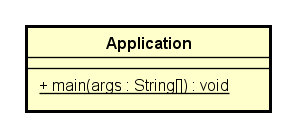
\includegraphics[scale=0.8,keepaspectratio]{img/server/Application.png}}
\caption{\nogloxy{swedesigner::server::Application}}
\end{figure}
\FloatBarrier
\begin{itemize}
\item \textbf{Descrizione}\\
Classe principale che consente l'avvio dell'applicazione spring.
\item \textbf{Utilizzo}\\
La classe viene utilizzata per avviare l'applicazione spring
\item \textbf{Metodi}:
\begin{itemize}
\item \nogloxy{\texttt{+ main(args: String[]): void}}
\\ Metodo principale che permette l'avvio dell'applicazione spring
\\ \textbf{Parametri}:
\begin{itemize}
\item \nogloxy{\texttt{args: String[]}}
\\ Rappresenta gli eventuali parametri passa al programma.
\end{itemize}
\end{itemize}
\end{itemize}
\subsection{\nogloxy{swedesigner::server::compiler}}
\label{\nogloxy{swedesigner::server::compiler}}
\subsubsection{Informazioni generali}
\begin{itemize}
\item \textbf{Descrizione}\\
Questo package contiene le classi adibite alla compilazione del codice sorgente in codice eseguibile (nel linguaggio target specifico). È stata prevista la possibilità di ampliare questo package inserendo al suo interno ulteriori package. All'interno di questo package è presente unicamente il package \texttt{java}.
\item \textbf{Padre}: \hyperref[\nogloxy{swedesigner::server}]{\nogloxy{\texttt{server}}}
\item \textbf{Package contenuti}:
\begin{itemize}
\item \hyperref[\nogloxy{swedesigner::server::compiler::java}]{\nogloxy{\texttt{java}}}\\
Questo package offre un'implementazione dell'interfaccia \texttt{Compiler} appartenente al package superiore. Possono essere aggiunti simili package per permettere la generazione in altri linguaggi.
\end{itemize}
\end{itemize}
\subsubsection{Classi}
\subsubsubsection{\nogloxy{swedesigner::server::compiler::Compiler}}
\label{\nogloxy{swedesigner::server::compiler::Compiler}}
\begin{figure}[h]
\centering
\nogloxy{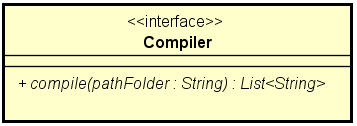
\includegraphics[scale=0.8,keepaspectratio]{img/server/Compiler.png}}
\caption{\nogloxy{swedesigner::server::compiler::Compiler}}
\end{figure}
\FloatBarrier
\begin{itemize}
\item \textbf{Descrizione}\\
questa interfaccia si occupa di fornire un oggetto compiler generico a chi lo richiede in modo da poter rendere entensibile il sistema aggiungendo un'implementazione concreta del compiler del linguaggio target desiderato.
\item \textbf{Utilizzo}\\
\textt{RequestHandlerController} ha una dipendenza verso \texttt{Compiler} in quanto chiederà a \textt{CompilerAssembler} una implementazione concreta di un \textt{Compiler} in base al linguaggio target. Il pattern realizzato con questa classe è una \emph{dependency injection}.
\item \textbf{Relazioni con altre classi}:
\begin{itemize}
\item \textit{IN} \hyperref[\nogloxy{swedesigner::server::compiler::java::JavaCompiler}]{\nogloxy{\texttt{JavaCompiler}}}\\
questa classe è una implementazione di \texttt{Compiler} che permette di creare un jar dal codice sorgente Java.
\item \textit{IN} \hyperref[\nogloxy{swedesigner::server::controller::RequestHandlerController}]{\nogloxy{\texttt{RequestHandlerController}}}\\
questa classe si occupa di ricevere le richieste REST provenienti dal client.
\end{itemize}
\item \textbf{Metodi}:
\begin{itemize}
\item \nogloxy{\texttt{+ compile(pathFolder: String): List<String>}}
\\ Compila un file sorgente in un eseguibile; ritorna una lista di errori di compilazione, se ce ne sono.
\\ \textbf{Parametri}:
\begin{itemize}
\item \nogloxy{\texttt{pathFolder: String}}
\\ Rappresenta la posizione della cartella nella quale sono presenti i file sorgente da compilare, relativi ad una particolare richiesta.
\end{itemize}
\end{itemize}
\end{itemize}
\subsection{\nogloxy{swedesigner::server::compiler::java}}
\label{\nogloxy{swedesigner::server::compiler::java}}
\subsubsection{Informazioni generali}
\begin{itemize}
\item \textbf{Descrizione}\\
Questo package offre un'implementazione dell'interfaccia \texttt{Compiler} appartenente al package superiore. Possono essere aggiunti simili package per permettere la generazione in altri linguaggi.
\item \textbf{Padre}: \hyperref[\nogloxy{swedesigner::server::compiler}]{\nogloxy{\texttt{compiler}}}
\end{itemize}
\subsubsection{Classi}
\subsubsubsection{\nogloxy{swedesigner::server::compiler::java::JavaCompiler}}
\label{\nogloxy{swedesigner::server::compiler::java::JavaCompiler}}
\begin{figure}[h]
\centering
\nogloxy{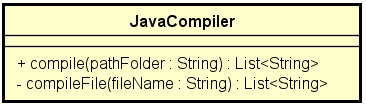
\includegraphics[scale=0.8,keepaspectratio]{img/server/JavaCompiler.png}}
\caption{\nogloxy{swedesigner::server::compiler::java::JavaCompiler}}
\end{figure}
\FloatBarrier
\begin{itemize}
\item \textbf{Descrizione}\\
questa classe è una implementazione di \texttt{Compiler} che permette di creare un jar dal codice sorgente Java.
\item \textbf{Utilizzo}\\
viene utilizzata da \texttt{CompilerAssembler} che ritorna un' istanza di essa quando richiesto.
\item \textbf{Relazioni con altre classi}:
\begin{itemize}
\item \textit{OUT} \hyperref[\nogloxy{swedesigner::server::compiler::Compiler}]{\nogloxy{\texttt{Compiler}}}\\
questa interfaccia si occupa di fornire un oggetto compiler generico a chi lo richiede in modo da poter rendere entensibile il sistema aggiungendo un'implementazione concreta del compiler del linguaggio target desiderato.
\end{itemize}
\item \textbf{Metodi}:
\begin{itemize}
\item \nogloxy{\texttt{+ compile(pathFolder: String): List<String>}}
\\ Crea i file compilati con estensione .class relativi ai file sorgente .java contenuti nella cartella che ha come percorso la stringa passata alla funzione stessa.
\\ \textbf{Parametri}:
\begin{itemize}
\item \nogloxy{\texttt{pathFolder: String}}
\\ Rappresenta la posizione della cartella nella quale sono presenti i file sorgente .java da compilare, relativi ad una particolare richiesta.
\end{itemize}
\item \nogloxy{\texttt{- compileFile(fileName: String): List<String>}}
\\ Crea il file compilato con estensione .class relativo al file sorgente .java passato come parametro.
\\ \textbf{Parametri}:
\begin{itemize}
\item \nogloxy{\texttt{fileName: String}}
\\ Rappresenta il percorso di un file con estensione .java.
\end{itemize}
\end{itemize}
\end{itemize}
\subsection{\nogloxy{swedesigner::server::controller}}
\label{\nogloxy{swedesigner::server::controller}}
\subsubsection{Informazioni generali}
\begin{itemize}
\item \textbf{Descrizione}\\
Questo package contiene i vari controller che implementano il pattern Front Controller fornito dal framework \emph{Spring}. Ogni controller dovrebbe occuparsi di gestire una richiesta e di rispondere opportunamente ad essa, attraverso l'interfaccia REST definita.
\item \textbf{Padre}: \hyperref[\nogloxy{swedesigner::server}]{\nogloxy{\texttt{server}}}
\end{itemize}
\subsubsection{Classi}
\subsubsubsection{\nogloxy{swedesigner::server::controller::RequestHandlerController}}
\label{\nogloxy{swedesigner::server::controller::RequestHandlerController}}
\begin{figure}[h]
\centering
\nogloxy{\includegraphics[scale=0.4,keepaspectratio]{img/server/handleGenerationRequestSequence.png}}
\caption{\nogloxy{diagramma di sequenza per le interazioni fra classi gestite dal metodo handleGenerationRequest}}
\end{figure}

\begin{figure}[h]
\centering
\nogloxy{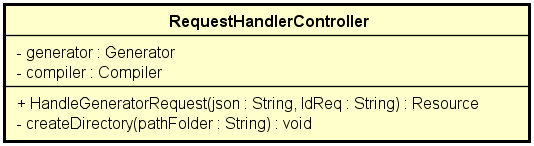
\includegraphics[scale=0.8,keepaspectratio]{img/server/RequestHandlerController.png}}
\caption{\nogloxy{swedesigner::server::controller::RequestHandlerController}}
\end{figure}
\FloatBarrier
\begin{itemize}
\item \textbf{Descrizione}\\
questa classe si occupa di ricevere le richieste REST provenienti dal client.
\item \textbf{Utilizzo}\\
essa deve gestire la richiesta di generazione di un progetto (attraverso file JSON) generando il codice e ritornandolo all'utente; inoltre essa deve restituire l'elenco degli stereotipi esistenti all'interno del server, con meta-attributi e meta-classi.
Richiama in ordine le varie classi addette alla generazione del codice, ovvero: un \texttt{Parser}, un \texttt{Generator}, un \texttt{Compiler} e infine il \texttt{Compressor}. 
\item \textbf{Relazioni con altre classi}:
\begin{itemize}
\item \textit{OUT} \hyperref[\nogloxy{swedesigner::server::compiler::Compiler}]{\nogloxy{\texttt{Compiler}}}\\
questa interfaccia si occupa di fornire un oggetto compiler generico a chi lo richiede in modo da poter rendere entensibile il sistema aggiungendo un'implementazione concreta del compiler del linguaggio target desiderato.
\item \textit{OUT} \hyperref[\nogloxy{swedesigner::server::generator::Generator}]{\nogloxy{\texttt{Generator}}}\\
questa interfaccia si occupa di fornire un oggetto \texttt{Generator} generico a chi lo richiede in modo da poter rendere entensibile il sistema aggiungendo un'implementazione concreta del generator del linguaggio target desiderato.
\item \textit{OUT} \hyperref[\nogloxy{swedesigner::server::parser::Parser}]{\nogloxy{\texttt{Parser}}}\\
questa classe si occupa di elaborare il file JSON proveniente dal client e di creare da esso un oggetto Java \texttt{ParsedProgram} strutturato in modo da poter essere facilmente convertito in codice.
\item \textit{OUT} \hyperref[\nogloxy{swedesigner::server::utility::Compressor}]{\nogloxy{\texttt{Compressor}}}\\
questa classe si occupa di creare e salvare su disco un archivio compresso contenente il progetto JSON, il codice sorgente e l'eseguibile generato che verrà poi messo a disposizione dell'utente che potrà scaricarlo.
\end{itemize}
\item \textbf{Attributi}:
\begin{itemize}
\item \nogloxy{\texttt{- compiler: Compiler}}
\\ Rifermento all'istanza di Compiler da utilizzare
\item \nogloxy{\texttt{- compressor: Compressor}}
\\ Riferimento all'istanza di Compressor da utilizzare.
\item \nogloxy{\texttt{- parser: Parser}}
\\ Riferimento all'istanza di Parser da utilizzare.
\item \nogloxy{\texttt{- uploadFolder: String}}
\\ Percorso della cartella all'interno del server nella quale memorizzare l'archivio zip da ritornare all'utente.
\item \nogloxy{\texttt{- generator: Generator}}
\\ Riferimento all'istanza di Generator da utilizzare.
\end{itemize}
\item \textbf{Metodi}:
\begin{itemize}
\item \nogloxy{\texttt{- createDirectory(pathFolder: String): void}}
\\ Gestisce la creazione di un'apposita cartella per la particolare richiesta ricevuta.
\\ \textbf{Parametri}:
\begin{itemize}
\item \nogloxy{\texttt{pathFolder: String}}
\\ Rappresenta la posizione della cartella che verrà creata relativa ad una particolare richiesta.
\end{itemize}
\item \nogloxy{\texttt{+ handleGenerationRequest(httpEntity: HttpEntity<String>): ResponseEntity<?>}}

\item \nogloxy{\texttt{+ HandleGenerationRequest(json: String, IdReq: String): void}}
\\ Il metodo riceve a partire dalla richiesta del client una stringa in formato .json ed anche l'id della richiesta stessa.
Il suo compito è:
\begin{itemize}
\item istanziare un oggetto Parser ed invocare su di esso il metodo createParsedProgram passando come argomento il file .json;
\item invocare il metodo generate sul proprio riferimento di tipo Generator passando come riferimento il ParsedProgram così ottenuto;
\item invocare sull'attributo compiler il metodo compile passando come argomento il riferimento alla cartella relativa alla particolare richiesta all'interno del server contenente i file .java;
\item istanziare un oggetto Compressor ed invocare su di esso il metodo zip per realizzare la risorsa .zip da ritornare all'utente;
\item ritornare in risposta all'utente il link a partire dal quale scaricare la risorsa .zip desiderata oppure un messaggio contenente gli errori rilevati dal Parser o dal Generator.
\end{itemize}
 \textbf{Parametri}:
\begin{itemize}
\item \nogloxy{\texttt{httpEntity: HttpEntity<String>}}
\\ Richiesta http contenente il file .json prodotto dall'editor.
\end{itemize}
\end{itemize}
\end{itemize}
\subsection{\nogloxy{swedesigner::server::generator}}
\label{\nogloxy{swedesigner::server::generator}}
\subsubsection{Informazioni generali}
\begin{itemize}
\item \textbf{Descrizione}\\
Questo package contiene le classi adibite alla trasformazione dal diagramma (rappresentato in oggetti Java derivati da oggetti JSON) a codice sorgente, nel linguaggio target specifico. È stata prevista la possibilità di ampliare questo package inserendo al suo interno ulteriori package. All'interno di questo package è presente unicamente il package \texttt{java}.
\item \textbf{Padre}: \hyperref[\nogloxy{swedesigner::server}]{\nogloxy{\texttt{server}}}
\item \textbf{Package contenuti}:
\begin{itemize}
\item \hyperref[\nogloxy{swedesigner::server::generator::java}]{\nogloxy{\texttt{java}}}\\
Questo package offre un'implementazione dell'interfaccia \texttt{Generator} appartenente al package superiore. Possono essere aggiunti simili package per permettere la generazione in altri linguaggi.
\end{itemize}
\end{itemize}
\subsubsection{Classi}
\subsubsubsection{\nogloxy{swedesigner::server::generator::Generator}}
\label{\nogloxy{swedesigner::server::generator::Generator}}
\begin{figure}[h]
\centering
\nogloxy{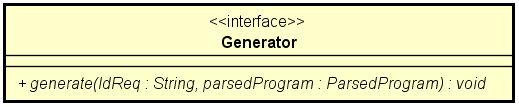
\includegraphics[scale=0.8,keepaspectratio]{img/server/Generator.png}}
\caption{\nogloxy{swedesigner::server::generator::Generator}}
\end{figure}
\FloatBarrier
\begin{itemize}
\item \textbf{Descrizione}\\
questa interfaccia si occupa di fornire un oggetto \texttt{Generator} generico a chi lo richiede in modo da poter rendere entensibile il sistema aggiungendo un'implementazione concreta del generator del linguaggio target desiderato.
\item \textbf{Utilizzo}\\
\texttt{RequestHandlerController} ha una dipendenza verso \texttt{Generator} in quanto chiederà a \texttt{GeneratorAssembler} una implementazione concreta di un \texttt{Generator} in base al linguaggio target. Il pattern realizzato con questa classe è una \emph{dependency injection}.
\item \textbf{Relazioni con altre classi}:
\begin{itemize}
\item \textit{IN} \hyperref[\nogloxy{swedesigner::server::controller::RequestHandlerController}]{\nogloxy{\texttt{RequestHandlerController}}}\\
questa classe si occupa di ricevere le richieste REST provenienti dal client.
\item \textit{IN} \hyperref[\nogloxy{swedesigner::server::generator::java::JavaGenerator}]{\nogloxy{\texttt{JavaGenerator}}}\\
questa classe è una implementazione di \texttt{Compiler} che permette di creare del codice sorgente Java da un \texttt{ParsedProgram}.
\item \textit{OUT} \hyperref[\nogloxy{swedesigner::server::project::ParsedElement}]{\nogloxy{\texttt{ParsedElement}}}\\
questa classe descrive il contratto di un elemento generico \texttt{Parsed}. Si specifica il metodo \texttt{RenderTemplate} che impone la necessità di implementarlo ad ogni classe sottostante.
\item \textit{OUT} \hyperref[\nogloxy{swedesigner::server::template::Template}]{\nogloxy{\texttt{Template}}}\\
questa interfaccia si occupa di fornire un oggetto template generico a chi lo richiede in modo da poter rendere estensibile il sistema aggiungendo un'implementazione concreta del template del linguaggio target desiderato.
\end{itemize}
\item \textbf{Metodi}:
\begin{itemize}
\item \nogloxy{\texttt{+ generate(idReq: String, parsedProgram: ParsedProgram): void}}
\\ Crea e salva i file sorgente del programma.
\\ \textbf{Parametri}:
\begin{itemize}
\item \nogloxy{\texttt{idReq: String}}
\\ Rappresenta l'identificatore della richiesta ricevuta.
\item \nogloxy{\texttt{parsedProgram: ParsedProgram}}
\\ Rappresenta l'oggetto ParsedProgram che sarà trasformato nel codice di un particolare linguaggio. 
\end{itemize}
\end{itemize}
\end{itemize}
\subsection{\nogloxy{swedesigner::server::generator::java}}
\label{\nogloxy{swedesigner::server::generator::java}}
\subsubsection{Informazioni generali}
\begin{itemize}
\item \textbf{Descrizione}\\
Questo package offre un'implementazione dell'interfaccia \texttt{Generator} appartenente al package superiore. Possono essere aggiunti simili package per permettere la generazione in altri linguaggi.
\item \textbf{Padre}: \hyperref[\nogloxy{swedesigner::server::generator}]{\nogloxy{\texttt{generator}}}
\end{itemize}
\subsubsection{Classi}
\subsubsubsection{\nogloxy{swedesigner::server::generator::java::JavaGenerator}}
\label{\nogloxy{swedesigner::server::generator::java::JavaGenerator}}
\begin{figure}[h]
\centering
\nogloxy{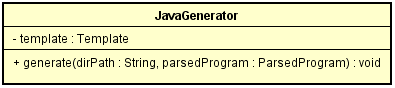
\includegraphics[scale=0.8,keepaspectratio]{img/server/JavaGenerator.png}}
\caption{\nogloxy{swedesigner::server::generator::java::JavaGenerator}}
\end{figure}
\FloatBarrier
\begin{itemize}
\item \textbf{Descrizione}\\
questa classe è una implementazione di \texttt{Compiler} che permette di creare del codice sorgente Java da un \texttt{ParsedProgram}.
\item \textbf{Utilizzo}\\
viene utilizzata da \texttt{CompilerAssembler} che ritorna un' istanza di essa quando richiesto.
\item \textbf{Relazioni con altre classi}:
\begin{itemize}
\item \textit{OUT} \hyperref[\nogloxy{swedesigner::server::generator::Generator}]{\nogloxy{\texttt{Generator}}}\\
questa interfaccia si occupa di fornire un oggetto \texttt{Generator} generico a chi lo richiede in modo da poter rendere entensibile il sistema aggiungendo un'implementazione concreta del generator del linguaggio target desiderato.
\end{itemize}
\item \textbf{Attributi}:
\begin{itemize}
\item \nogloxy{\texttt{- template: Template}}
\\ Riferimento alla particolare istanza di Template da utilizzare.
\end{itemize}
\item \textbf{Metodi}:
\begin{itemize}
\item \nogloxy{\texttt{+ generate(parsedProgram: ParsedProgram, idReq: String): void}}
\\ Crea e salva i file sorgente .java del programma.
\\ \textbf{Parametri}:
\begin{itemize}
\item \nogloxy{\texttt{parsedProgram: ParsedProgram}}
\\ Rappresenta l'oggetto ParsedProgram che sarà trasformato in codice Java. 
\item \nogloxy{\texttt{idReq: String}}
\\ Rappresenta l'identificatore della richiesta ricevuta.
\end{itemize}
\end{itemize}
\end{itemize}
\subsection{\nogloxy{swedesigner::server::parser}}
\label{\nogloxy{swedesigner::server::parser}}
\subsubsection{Informazioni generali}
\begin{itemize}
\item \textbf{Descrizione}\\
Questo package presenta le classi utili all'attività di parsing dei dati ricevuti dai client.
\item \textbf{Padre}: \hyperref[\nogloxy{swedesigner::server}]{\nogloxy{\texttt{server}}}
\end{itemize}
\subsubsection{Classi}
\subsubsubsection{\nogloxy{swedesigner::server::parser::Parser}}
\label{\nogloxy{swedesigner::server::parser::Parser}}
\begin{figure}[H]
\centering
\nogloxy{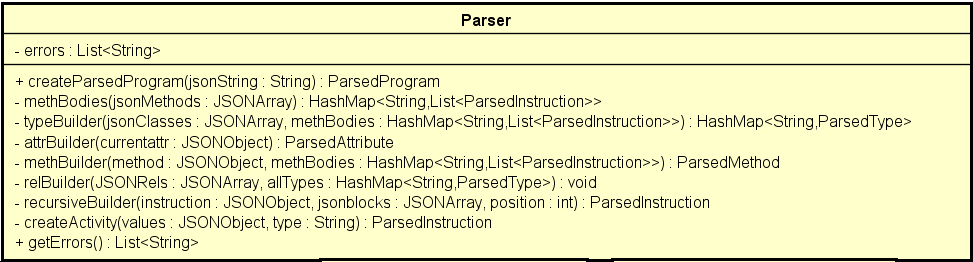
\includegraphics[scale=0.4,keepaspectratio]{img/server/Parser.png}}
\caption{\nogloxy{swedesigner::server::parser::Parser}}
\end{figure}
\begin{figure}[h]
\centering
\nogloxy{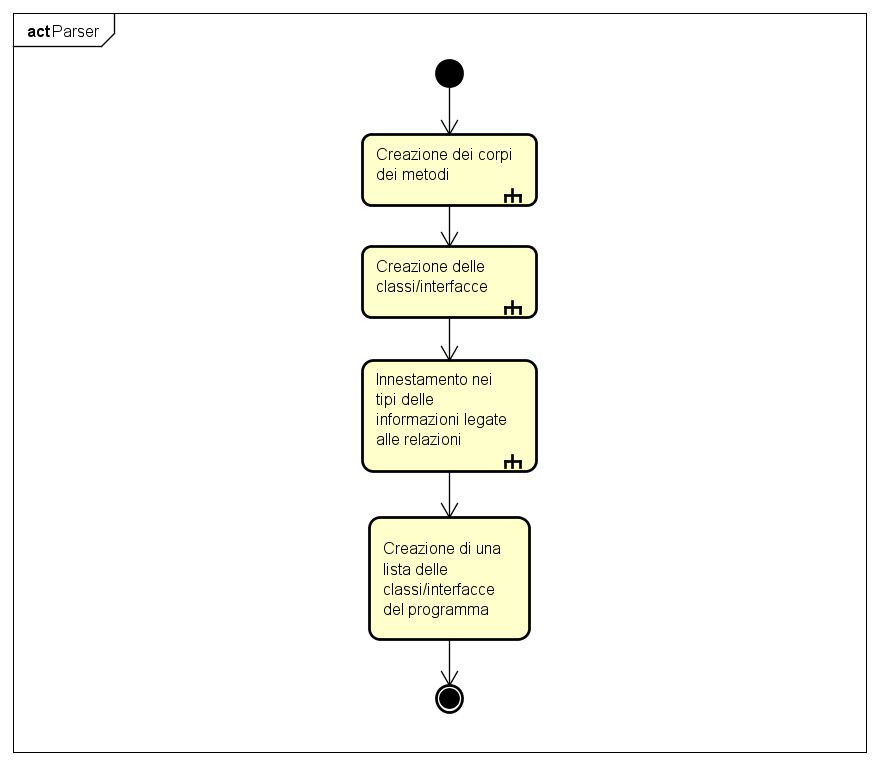
\includegraphics[scale=0.4,keepaspectratio]{img/server/ParserActivity.png}}
\caption{\nogloxy{diagramma di attività per il flusso di esecuzione del metodo createParsedProgram della classe Parser}}
\end{figure}
\begin{figure}[h]
\centering
\nogloxy{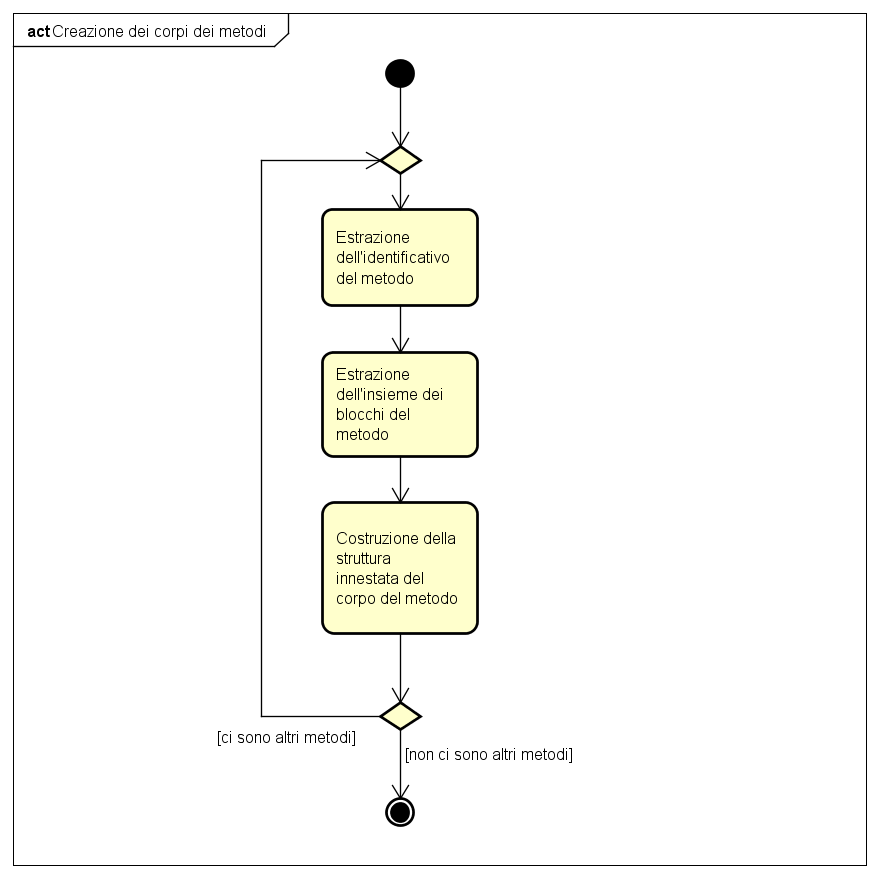
\includegraphics[scale=0.4,keepaspectratio]{img/server/CreazioneCorpiMetodiActivity.png}}
\caption{\nogloxy{diagramma di attività per il flusso di esecuzione del metodo methBuilder della classe Parser}}
\end{figure}
\begin{figure}[h]
\centering
\nogloxy{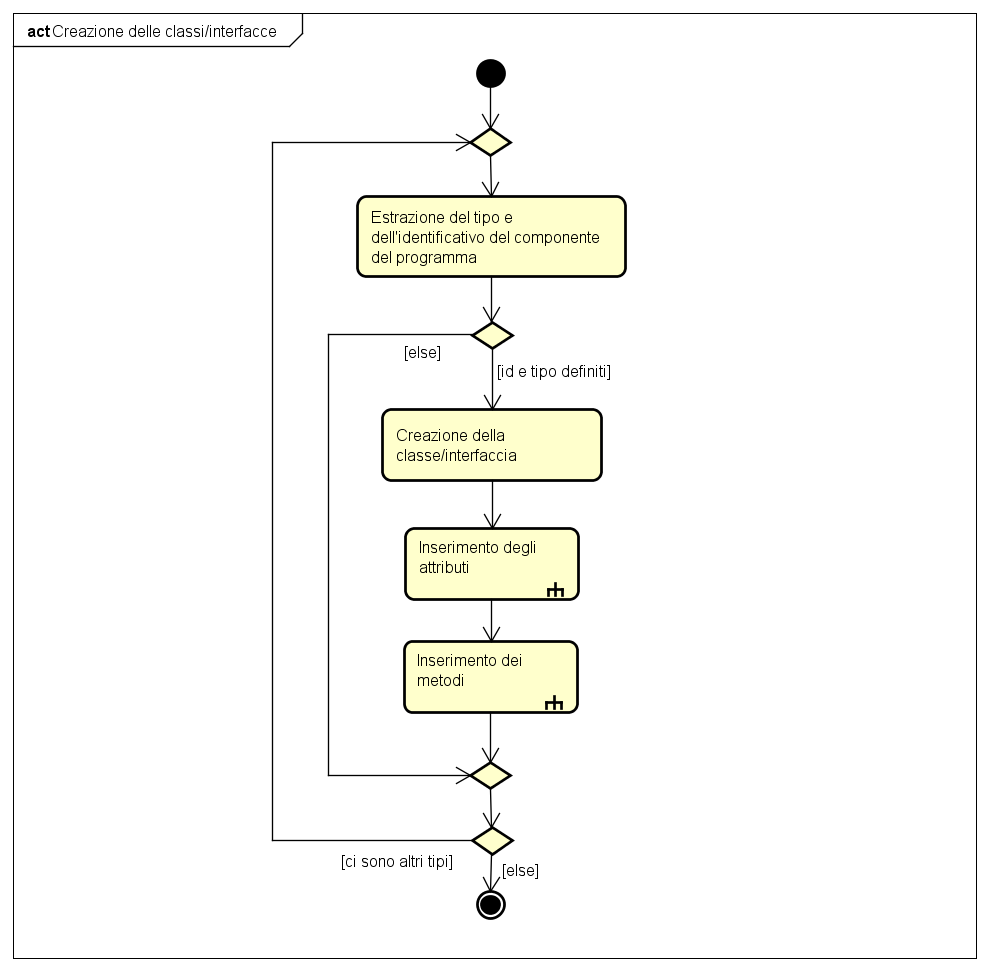
\includegraphics[scale=0.4,keepaspectratio]{img/server/CreazioneTipiActivity.png}}
\caption{\nogloxy{diagramma di attività per il flusso di esecuzione del metodo typeBuilder della classe Parser}}
\end{figure}
\begin{figure}[h]
\centering
\nogloxy{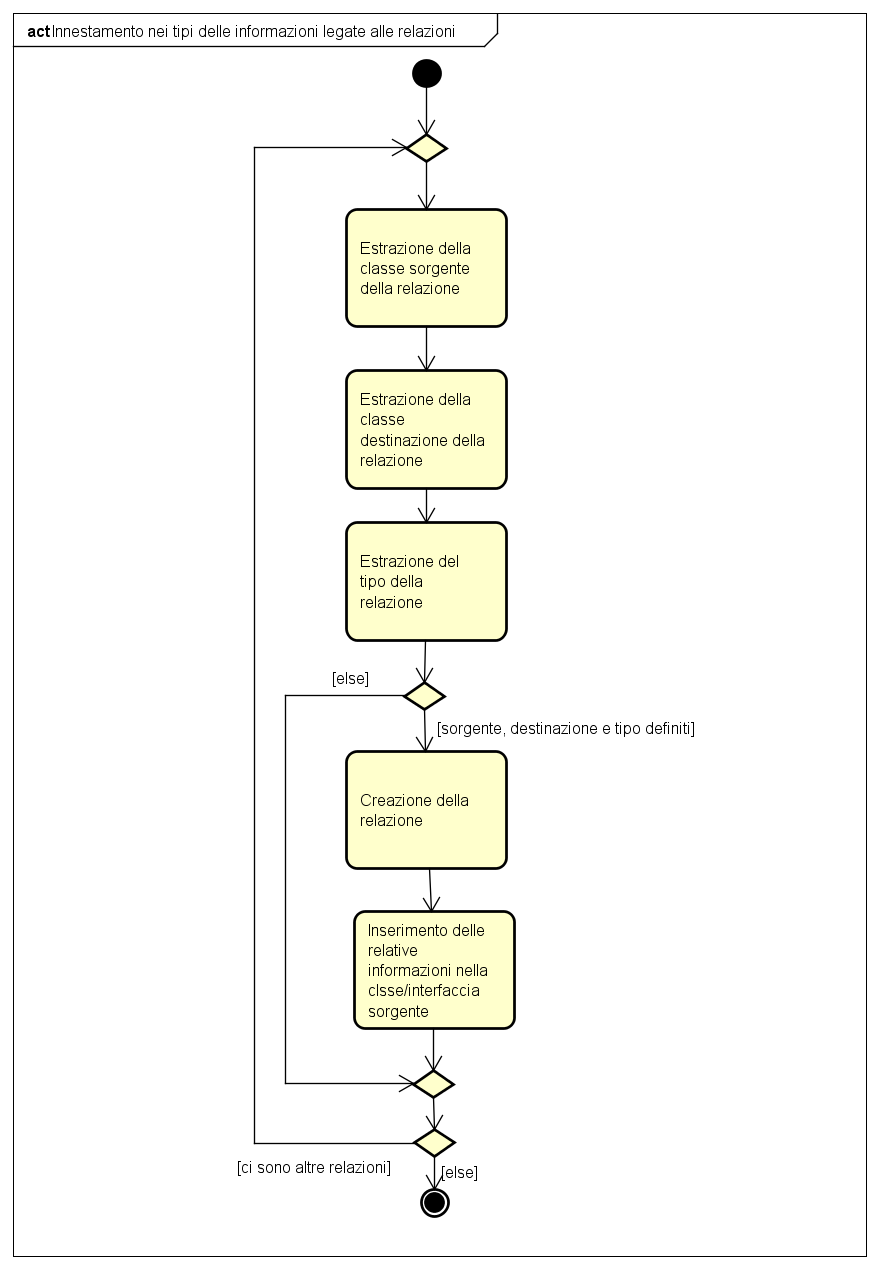
\includegraphics[scale=0.4,keepaspectratio]{img/server/CreazioneRelazioniActivity.png}}
\caption{\nogloxy{diagramma di attività per il flusso di esecuzione del metodo relBuilder della classe Parser}}
\end{figure}
\FloatBarrier
\begin{itemize}
\item \textbf{Descrizione}\\
questa classe si occupa di elaborare il file JSON proveniente dal client e di creare da esso un oggetto Java \texttt{ParsedProgram} strutturato in modo da poter essere facilmente convertito in codice.
\item \textbf{Utilizzo}\\
viene utilizzata da \texttt{RequestHandlerController} che ne crea un istanza e ne chiama i metodi per elaborare il JSON. \texttt{Parser} inoltre crea istanze di \texttt{ParsedElement} e ritorna a controller un'istanza di \texttt{ParsedProgram}.
\item \textbf{Relazioni con altre classi}:
\begin{itemize}
\item \textit{IN} \hyperref[\nogloxy{swedesigner::server::controller::RequestHandlerController}]{\nogloxy{\texttt{RequestHandlerController}}}\\
questa classe si occupa di ricevere le richieste REST provenienti dal client.
\item \textit{OUT} \hyperref[\nogloxy{swedesigner::server::project::ParsedProgram}]{\nogloxy{\texttt{ParsedProgram}}}\\
questa classe rappresenta l'entità che possiede al suo interno tutte le componenti di un progetto. Essa possiede più \texttt{ParsedType}.
\end{itemize}
\item \textbf{Attributi}:
\begin{itemize}
\item \nogloxy{\texttt{- errors: List<String>}}
\\ è la lista in cui vengono memorizzati gli errori rilevati durante l'elaborazione della stringa json.
\end{itemize}
\item \textbf{Metodi}:
\begin{itemize}
\item \nogloxy{\texttt{- attrBuilder(currentAttr: JSONObject): ParsedAttribute}}
\\ Costruisce l'oggetto relativo ad uno dei campi dati delle classi del programma.
\\ \textbf{Parametri}:
\begin{itemize}
\item \nogloxy{\texttt{currentAttr: JSONObject}}
\\ Rappresenta un attributo/campo dato in forma JSON.
\end{itemize}
\item \nogloxy{\texttt{- createActivity(value: JSONObject, type: String): ParsedInstruction}}
\\ Costruisce l'oggetto relativo ad una particolare istruzione del programma.
\\ \textbf{Parametri}:
\begin{itemize}
\item \nogloxy{\texttt{value: JSONObject}}
\\ Rappresenta un particolare blocco di istruzioni in forma JSON.
\item \nogloxy{\texttt{type: String}}
\\ Rappresenta il tipo di un particolare blocco di istruzioni.
\end{itemize}
\item \nogloxy{\texttt{+ createParsedProgram(jsonString: String): ParsedProgram}}
\\ Traduce la stringa json in una corrispondente struttura ad oggetti.
\\ \textbf{Parametri}:
\begin{itemize}
\item \nogloxy{\texttt{jsonString: String}}
\\ Rappresenta il contenuto del file .json in forma di stringa.
\end{itemize}
\item \nogloxy{\texttt{+ getErrors(): List<String>}}
\\ Ritorna l'attributo errors.
\item \nogloxy{\texttt{- methBodies(jsonMethods: JSONArray): HashMap<String, List<ParsedInstruction>}}
\\ Crea la struttura ad oggetti relativa al corpo dei metodi del programma.
\\ \textbf{Parametri}:
\begin{itemize}
\item \nogloxy{\texttt{jsonMethods: JSONArray}}
\\ Rappresenta l'insieme dei corpi dei metodi in forma JSON.
\end{itemize}
\item \nogloxy{\texttt{- methBuilder(method: JSONObject, methBodies: HashMap<String, List<ParsedInstruction>): ParsedMethod}}
\\ Realizza l'oggetto contenente le informazioni relative all'intestazione di uno dei metodi del programma
\\ \textbf{Parametri}:
\begin{itemize}
\item \nogloxy{\texttt{method: JSONObject}}
\\ Rappresenta la segnatura di un metodo in forma JSON.
\item \nogloxy{\texttt{methBodies: HashMap<String, List<ParsedInstruction>}}
\\ Rappresenta la corrispondenza tra id di un metodo e il suo corpo in forma di ParsedInstruction.
\end{itemize}
\item \nogloxy{\texttt{- recursiveBuilder(instruction: JSONObject, jsonBlock: JSONArray, position: int): ParsedInstruction}}
\\ Crea il contenuto del corpo di una delle istruzioni non atomiche del programma.
\\ \textbf{Parametri}:
\begin{itemize}
\item \nogloxy{\texttt{instruction: JSONObject}}
\\ Rappresenta un'istruzione in forma JSON.
\item \nogloxy{\texttt{jsonBlock: JSONArray}}
\\ Rappresenta l'insieme di blocchi, in forma JSON, che forma il corpo di un metodo.
\item \nogloxy{\texttt{position: int}}
\\ Indica la posizione da cui ricercare i successivi blocchi di istruzioni.
\end{itemize}
\item \nogloxy{\texttt{- relBuilder(jsonRels: JSONArray, allTypes: HashMap<String, List<ParsedType>): void}}
\\ Aggiunge nei tipi precedentemente creati le informazioni relative alle relazioni tra essi.
\\ \textbf{Parametri}:
\begin{itemize}
\item \nogloxy{\texttt{jsonRels: JSONArray}}
\\ Rappresenta l'insieme delle relazioni in forma JSON.
\item \nogloxy{\texttt{allTypes: HashMap<String, List<ParsedType>}}
\\ Rappresenta la corrispondenza tra id di un tipo e il suo codice in forma di ParsedType.
\end{itemize}
\item \nogloxy{\texttt{- typeBuilder(jsonClasses: JSONArray, methBodies: HashMap<String, List<ParsedInstruction>): HashMap<String, List<ParsedType>}}
\\ Costruisce gli oggetti relativi ai tipi del programma (classi ed intefacce).
\\ \textbf{Parametri}:
\begin{itemize}
\item \nogloxy{\texttt{jsonClasses: JSONArray}}
\\ Rappresenta l'insieme dei tipi in forma JSON.
\item \nogloxy{\texttt{methBodies: HashMap<String, List<ParsedInstruction>}}
\\ Rappresenta la corrispondenza tra id di un metodo e il suo corpo in forma di ParsedInstruction.
\end{itemize}
\end{itemize}
\end{itemize}
\subsection{\nogloxy{swedesigner::server::project}}
\label{\nogloxy{swedesigner::server::project}}
\subsubsection{Informazioni generali}
\begin{itemize}
\item \textbf{Descrizione}\\
Questo package contiene al suo interno le classi utili a rappresentare un progetto UML. Il package parser necessita di questo package per poter dare in output un programma rappresentato in memoria come oggetti Java. Per chiarezza e per evitare l'uso di keyword riservate dal linguaggio Java, all'inizio del nome di queste classi è inserito il prefisso \texttt{Parsed} (e.g. \texttt{ParsedClass}).
\item \textbf{Padre}: \hyperref[\nogloxy{swedesigner::server}]{\nogloxy{\texttt{server}}}
\end{itemize}
\subsubsection{Classi}
\subsubsubsection{\nogloxy{swedesigner::server::project::ParsedAttribute}}
\label{\nogloxy{swedesigner::server::project::ParsedAttribute}}
\begin{figure}[h]
\centering
\nogloxy{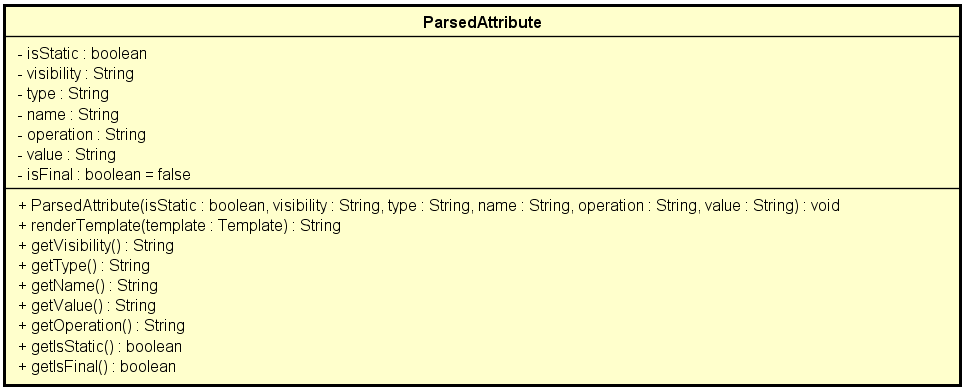
\includegraphics[scale=0.5,keepaspectratio]{img/server/ParsedAttribute.png}}
\caption{\nogloxy{swedesigner::server::project::ParsedAttribute}}
\end{figure}
\FloatBarrier
\begin{itemize}
\item \textbf{Descrizione}\\
questa classe rappresenta un singolo attributo, memorizzando il nome della variabile, la sua visibilità e il suo valore di default. Viene utilizzata anche per rappresentare i parametri dei metodi.
% Tuttavia, ciò non vale per attributi statici. 
% Nella \emph{Definizione_di_prodotto_v_1_0_0} [RIFERIMENTO] sarà esplicitata l'implementazione di dettaglio decisa.
\item \textbf{Utilizzo}\\
questa classe è usata da \texttt{ParsedMethod},  \texttt{ParsedClass} e \texttt{ParsedInterface} (le interfacce possono però contenere solo costanti di classe).
Questa classe implementa l'interfaccia \texttt{ParsedElement}.
Nota: Memorizzare il valore di questo attributo risulta superfluo, in quanto questo può essere impostato da un \texttt{ParsedAssignment}. 

\item \textbf{Relazioni con altre classi}:
\begin{itemize}
\item \textit{IN} \hyperref[\nogloxy{swedesigner::server::project::ParsedClass}]{\nogloxy{\texttt{ParsedClass}}}\\
questa classe estende la classe astratta \texttt{ParsedType}, imponendo al suo interno la presenza di una lista di \texttt{ParsedAttribute}. 
\item \textit{IN} \hyperref[\nogloxy{swedesigner::server::project::ParsedMethod}]{\nogloxy{\texttt{ParsedMethod}}}\\
questa classe rappresenta un metodo come insieme di istruzioni \texttt{ParsedIstruction} e un insieme di \texttt{ParsedAttribute} come parametri del metodo.
\item \textit{IN} \hyperref[\nogloxy{swedesigner::server::project::ParsedMethod}]{\nogloxy{\texttt{ParsedMethod}}}\\
questa classe rappresenta un metodo come insieme di istruzioni \texttt{ParsedIstruction} e un insieme di \texttt{ParsedAttribute} come parametri del metodo.
\item \textit{OUT} \hyperref[\nogloxy{swedesigner::server::project::ParsedElement}]{\nogloxy{\texttt{ParsedElement}}}\\
questa classe descrive il contratto di un elemento generico \texttt{Parsed}. Si specifica il metodo \texttt{RenderTemplate} che impone la necessità di implementarlo ad ogni classe sottostante.
\end{itemize}
\item \textbf{Attributi}:
\begin{itemize}
\item \nogloxy{\texttt{- isFinal: boolean}}
\\ Indica se l'oggetto ParsedAttribute è costante.
\item \nogloxy{\texttt{- isStatic: boolean}}
\\ Indica se il ParsedAttribute è un oggetto statico.
\item \nogloxy{\texttt{- name: String}}
\\ Indica il nome dell'oggetto ParsedAttribute.
\item \nogloxy{\texttt{- operation: String}}
\\ Indica l'operatore di assegnazione del valore iniziale dell'oggetto ParsedAttribute.
\item \nogloxy{\texttt{- type: String}}
\\ Indica il tipo dell'oggetto ParsedAttribute.
\item \nogloxy{\texttt{- value: String}}
\\ Indica il valore iniziale dell'oggetto ParsedAttribute.
\item \nogloxy{\texttt{- visibility: String}}
\\ Indica la visibilità dell'oggetto ParsedAttribute.
\end{itemize}
\item \textbf{Metodi}:
\begin{itemize}
\item \nogloxy{\texttt{+ getIsFinal(): boolean}}
\\ Ritorna informazioni relative alla natura costante di un oggetto ParsedAttribute.
\item \nogloxy{\texttt{+ getIsStatic(): boolean}}
\\ Ritorna informazioni riguardanti la staticità di un oggetto ParsedAttribute.
\item \nogloxy{\texttt{+ getName(): String}}
\\ Ritorna il nome di un oggetto ParsedAttribute.
\item \nogloxy{\texttt{+ getOperation(): String}}
\\ Ritorna l'operatore di assegnazione del valore iniziale di un oggetto ParsedAttribute.
\item \nogloxy{\texttt{+ getType(): String}}
\\ Ritorna il tipo di un oggetto ParsedAttribute.
\item \nogloxy{\texttt{+ getValue(): String}}
\\ Ritorna il valore iniziale di un oggetto ParsedAttribute.
\item \nogloxy{\texttt{+ getVisibility(): String}}
\\ Ritorna la visibilità di un oggetto ParsedAttribute.
\item \nogloxy{\texttt{+ ParsedAttribute(isStatic: boolean, visibility: String, type: String, name: String, operation: String, value: String)}}
\\ Costruisce un oggetto ParsedAttribute.
\\ \textbf{Parametri}:
\begin{itemize}
\item \nogloxy{\texttt{isStatic: boolean}}
\\ Indica se il ParsedAttribute che si sta creando è un oggetto statico.
\item \nogloxy{\texttt{visibility: String}}
\\ Indica la visibilità dell'oggetto ParsedAttribute che si sta creando.
\item \nogloxy{\texttt{type: String}}
\\ Indica il tipo dell'oggetto ParsedAttribute che si sta creando.
\item \nogloxy{\texttt{name: String}}
\\  Indica il nome dell'oggetto ParsedAttribute che si sta creando.
\item \nogloxy{\texttt{operation: String}}
\\ Indica l'operatore di assegnazione del valore iniziale dell'oggetto ParsedAttribute che si sta creando.
\item \nogloxy{\texttt{value: String}}
\\ Indica il valore iniziale dell'oggetto ParsedAttribute che si sta creando.
\end{itemize}
\item \nogloxy{\texttt{+ renderTemplate(template: Template): String}}
\\ Traduce l'oggetto ParsedAttribute in una stringa che rappresenta il codice di un particolare linguaggio di programmazione.
\\ \textbf{Parametri}:
\begin{itemize}
\item \nogloxy{\texttt{template: Template}}
\\ Riferimento alla particolare istanza di Template da utilizzare.
\end{itemize}
\end{itemize}
\end{itemize}

\subsubsubsection{\nogloxy{swedesigner::server::project::ParsedClass}}
\label{\nogloxy{swedesigner::server::project::ParsedClass}}
\begin{figure}[h]
\centering
\nogloxy{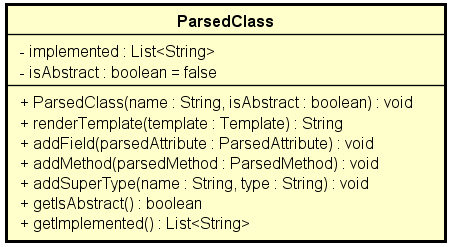
\includegraphics[scale=0.8,keepaspectratio]{img/server/ParsedClass.png}}
\caption{\nogloxy{swedesigner::server::project::ParsedClass}}
\end{figure}
\FloatBarrier
\begin{itemize}
\item \textbf{Descrizione}\\
questa classe estende la classe astratta \texttt{ParsedType}, imponendo al suo interno la presenza di una lista di \texttt{ParsedAttribute}. 
\item \textbf{Utilizzo}\\
questa classe è creata tramite la \texttt{ElementFactory} durante il parsing del progetto e inserita all'interno di \texttt{ParsedProgram}.
\item \textbf{Classi ereditate}:
\begin{itemize}
\item \hyperref[\nogloxy{swedesigner::server::project::ParsedType}]{\nogloxy{\texttt{ParsedType}}}
\end{itemize}
\item \textbf{Relazioni con altre classi}:
\begin{itemize}
\item \textit{IN} \hyperref[\nogloxy{swedesigner::server::project::ParsedException}]{\nogloxy{\texttt{ParsedException}}}\\
Questa classe rappresenta una eccezione che viene sollevata nel momento in cui viene identificata una illegalità nel parsing della stringa in formato .json
\item \textit{OUT} \hyperref[\nogloxy{swedesigner::server::project::ParsedAttribute}]{\nogloxy{\texttt{ParsedAttribute}}}\\
questa classe rappresenta un singolo attributo, memorizzando il nome della variabile, la sua visibilità e il suo valore di default. Viene utilizzata anche per rappresentare i parametri dei metodi.
% Tuttavia, ciò non vale per attributi statici. 
% Nella \emph{Definizione_di_prodotto_v_1_0_0} [RIFERIMENTO] sarà esplicitata l'implementazione di dettaglio decisa.
\item \textit{OUT} \hyperref[\nogloxy{swedesigner::server::project::ParsedMethod}]{\nogloxy{\texttt{ParsedMethod}}}\\
questa classe rappresenta un metodo come insieme di istruzioni \texttt{ParsedIstruction} e un insieme di \texttt{ParsedAttribute} come parametri del metodo.
\end{itemize}
\item \textbf{Attributi}:
\begin{itemize}
\item \nogloxy{\texttt{- implemented: List<String>}}
\\ Indica i nomi delle interfacce implementate.
\item \nogloxy{\texttt{- isAbstract: boolean}}
\\ Indica se l'oggetto ParsedClass è astratto o meno, ovvero se ha delle componenti che devono essere implementate.
\end{itemize}
\item \textbf{Metodi}:
\begin{itemize}
\item \nogloxy{\texttt{+ addField(parsedAttribute: ParsedAttribute): void}}
\\ Aggiunge all'oggetto ParsedClass un attributo rappresentato da un oggetto ParsedAttribute.
\\ \textbf{Parametri}:
\begin{itemize}
\item \nogloxy{\texttt{parsedAttribute: ParsedAttribute}}
\\ Indica il ParsedAttribute che deve essere aggiunto alla ParsedClass.
\end{itemize}
\item \nogloxy{\texttt{+ addMethod(parsedMethod: ParsedMethod): void}}
\\ Aggiunge ad un oggetto ParsedClass un metodo rappresentato da un oggetto ParsedMethod.
\\ \textbf{Parametri}:
\begin{itemize}
\item \nogloxy{\texttt{parsedMethod: ParsedMethod}}
\\ Indica il ParsedMethod che deve essere aggiunto alla ParsedClass.
\end{itemize}
\item \nogloxy{\texttt{+ addSupertype(name: String, type: String): void}}
\\ Aggiunge il nome di uno dei "supertipi" diretti dell'oggetto ParsedClass.
\\ \textbf{Parametri}:
\begin{itemize}
\item \nogloxy{\texttt{name: String}}
\\ Indica il nome del "supertipo" che deve essere implementato o esteso.
\item \nogloxy{\texttt{type: String}}
\\ Indica il tipo, classe o interfaccia, che deve essere rispettivamente esteso o implementato.
\end{itemize}
\item \nogloxy{\texttt{+ getImplemented(): List<String>}}
\\ Ritorna i nomi delle interfacce implementate.
\item \nogloxy{\texttt{+ getIsAbstract(): boolean}}
\\ Ritorna informazioni relative astrattezza dell'oggetto ParsedClass.
\item \nogloxy{\texttt{+ ParsedClass(name: String, isAbstract: boolean)}}
\\ Costruisce un oggetto ParsedClass.
\\ \textbf{Parametri}:
\begin{itemize}
\item \nogloxy{\texttt{name: String}}
\\ Rappresenta il nome del particolare oggetto ParsedClass che si sta creando.
\item \nogloxy{\texttt{isAbstract: boolean}}
\\ Indica se l'oggetto ParsedClass che si sta creando è astratto o meno.
\end{itemize}
\item \nogloxy{\texttt{+ renderTemplate(template: Template): String}}
\\ Traduce l'oggetto ParsedClass in una stringa che rappresenta il codice di un particolare linguaggio di programmazione.
\\ \textbf{Parametri}:
\begin{itemize}
\item \nogloxy{\texttt{template: Template}}
\\ Riferimento alla particolare istanza di Template da utilizzare.
\end{itemize}
\end{itemize}
\end{itemize}

\subsubsubsection{\nogloxy{swedesigner::server::project::ParsedCustom}}
\label{\nogloxy{swedesigner::server::project::ParsedCustom}}
\begin{figure}[h]
\centering
\nogloxy{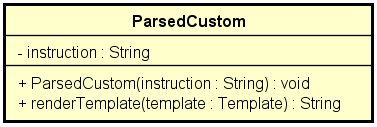
\includegraphics[scale=0.8,keepaspectratio]{img/server/ParsedCustom.png}}
\caption{\nogloxy{swedesigner::server::project::ParsedCustom}}
\end{figure}
\FloatBarrier
\begin{itemize}
\item \textbf{Descrizione}\\
questa classe descrive il comportamento di un blocco di codice custom, scritto nel linguaggio target.	
\item \textbf{Utilizzo}\\
dispone della possibilità di effettuare il render di un template in ingresso.
\item \textbf{Classi ereditate}:
\begin{itemize}
\item \hyperref[\nogloxy{swedesigner::server::project::ParsedInstruction}]{\nogloxy{\texttt{ParsedInstruction}}}
\end{itemize}
\item \textbf{Attributi}:
\begin{itemize}
\item \nogloxy{\texttt{- instruction: String}}
\\ Indica il codice inserito dall'utente in blocco custom.
\end{itemize}
\item \textbf{Metodi}:
\begin{itemize}
\item \nogloxy{\texttt{+ ParsedCustom(instruction: String)}}
\\ Costruisce un oggetto ParsedCustom.
\\ \textbf{Parametri}:
\begin{itemize}
\item \nogloxy{\texttt{instruction: String}}
\\ Indica l'insieme di istruzioni inserite dall'utente.
\end{itemize}
\item \nogloxy{\texttt{+ renderTemplate(template: Template): String}}
\\ Traduce l'oggetto ParsedCustom in una stringa che rappresenta il codice di un particolare linguaggio di programmazione.
\\ \textbf{Parametri}:
\begin{itemize}
\item \nogloxy{\texttt{template: Template}}
\\ Riferimento alla particolare istanza di Template da utilizzare.
\end{itemize}
\end{itemize}
\end{itemize}

\subsubsubsection{\nogloxy{swedesigner::server::project::ParsedElement}}
\label{\nogloxy{swedesigner::server::project::ParsedElement}}
\begin{figure}[h]
\centering
\nogloxy{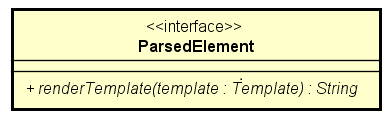
\includegraphics[scale=0.8,keepaspectratio]{img/server/ParsedElement.png}}
\caption{\nogloxy{swedesigner::server::project::ParsedElement}}
\end{figure}
\FloatBarrier
\begin{itemize}
\item \textbf{Descrizione}\\
questa classe descrive il contratto di un elemento generico \texttt{Parsed}. Si specifica il metodo \texttt{RenderTemplate} che impone la necessità di implementarlo ad ogni classe sottostante.
\item \textbf{Utilizzo}\\
questa interfaccia è usata da \texttt{ElementFactory}, la quale fornisce un metodo per creare nuovi elementi secondo il design pattern Factory. %[RIFERIMENTO AD APPENDICE].
\item \textbf{Sottoclassi}:
\begin{itemize}
\item \hyperref[\nogloxy{swedesigner::server::project::ParsedMethod}]{\nogloxy{\texttt{ParsedMethod}}}
\end{itemize}
\item \textbf{Relazioni con altre classi}:
\begin{itemize}
\item \textit{IN} \hyperref[\nogloxy{swedesigner::server::generator::Generator}]{\nogloxy{\texttt{Generator}}}\\
questa interfaccia si occupa di fornire un oggetto \texttt{Generator} generico a chi lo richiede in modo da poter rendere entensibile il sistema aggiungendo un'implementazione concreta del generator del linguaggio target desiderato.
\item \textit{IN} \hyperref[\nogloxy{swedesigner::server::project::ParsedAttribute}]{\nogloxy{\texttt{ParsedAttribute}}}\\
questa classe rappresenta un singolo attributo, memorizzando il nome della variabile, la sua visibilità e il suo valore di default. Viene utilizzata anche per rappresentare i parametri dei metodi.
% Tuttavia, ciò non vale per attributi statici. 
% Nella \emph{Definizione_di_prodotto_v_1_0_0} [RIFERIMENTO] sarà esplicitata l'implementazione di dettaglio decisa.
\item \textit{IN} \hyperref[\nogloxy{swedesigner::server::project::ParsedInstruction}]{\nogloxy{\texttt{ParsedInstruction}}}\\
questa classe astratta rappresenta la singola istruzione contenuta all'interno di un metodo. Essa è estesa dalle istruzioni specifiche (e.g. \texttt{ParsedIf}, \texttt{ParsedWhile}, etc.)
\item \textit{IN} \hyperref[\nogloxy{swedesigner::server::project::ParsedMethod}]{\nogloxy{\texttt{ParsedMethod}}}\\
questa classe rappresenta un metodo come insieme di istruzioni \texttt{ParsedIstruction} e un insieme di \texttt{ParsedAttribute} come parametri del metodo.
\item \textit{IN} \hyperref[\nogloxy{swedesigner::server::project::ParsedMethod}]{\nogloxy{\texttt{ParsedMethod}}}\\
questa classe rappresenta un metodo come insieme di istruzioni \texttt{ParsedIstruction} e un insieme di \texttt{ParsedAttribute} come parametri del metodo.
\item \textit{IN} \hyperref[\nogloxy{swedesigner::server::project::ParsedType}]{\nogloxy{\texttt{ParsedType}}}\\
questa classe astratta definisce un contratto comune tra le classi \texttt{ParsedInterface} e \texttt{ParsedClass}. 
\end{itemize}
\item \textbf{Metodi}:
\begin{itemize}
\item \nogloxy{\texttt{+ renderTemplate(template: Template): String}}
\\ Traduce l'oggetto ParsedElement in una stringa che rappresenta il codice di un particolare linguaggio di programmazione.
\\ \textbf{Parametri}:
\begin{itemize}
\item \nogloxy{\texttt{template: Template}}
\\ Riferimento alla particolare istanza di Template da utilizzare.
\end{itemize}
\end{itemize}
\end{itemize}

\subsubsubsection{\nogloxy{swedesigner::server::project::ParsedElse}}
\label{\nogloxy{swedesigner::server::project::ParsedElse}}
\begin{figure}[h]
\centering
\nogloxy{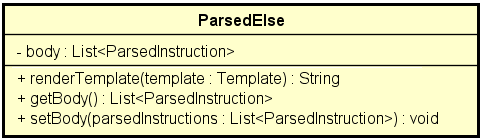
\includegraphics[scale=0.8,keepaspectratio]{img/server/ParsedElse.png}}
\caption{\nogloxy{swedesigner::server::project::ParsedElse}}
\end{figure}
\FloatBarrier
\begin{itemize}
\item \textbf{Descrizione}\\
questa classe descrive il comportamento di un blocco \texttt{else}.
\item \textbf{Utilizzo}\\
dispone della possibilità di effettuare il render di un template in ingresso.
\item \textbf{Classi ereditate}:
\begin{itemize}
\item \hyperref[\nogloxy{swedesigner::server::project::ParsedInstruction}]{\nogloxy{\texttt{ParsedInstruction}}}
\end{itemize}
\item \textbf{Attributi}:
\begin{itemize}
\item \nogloxy{\texttt{- body: List<ParsedInstruction>}}
\\ Indica l'insieme di istruzioni contenute nel corpo del corrispondente oggetto ParsedElse.
\end{itemize}
\item \textbf{Metodi}:
\begin{itemize}
\item \nogloxy{\texttt{+ getBody(): List<ParsedInstruction>}}
\\ Ritorna l'insieme di istruzioni che compongono il corpo del relativo oggetto ParsedElse.
\item \nogloxy{\texttt{+ renderTemplate(template: Template): String}}
\\ Traduce l'oggetto ParsedElse in una stringa che rappresenta il codice di un particolare linguaggio di programmazione.
\\ \textbf{Parametri}:
\begin{itemize}
\item \nogloxy{\texttt{template: Template}}
\\ Riferimento alla particolare istanza di Template da utilizzare.
\end{itemize}
\item \nogloxy{\texttt{+ setBody(parsedInstructions: List<ParsedInstruction>): void}}
\\ Inserisce nel campo dati body del ParsedElse un insieme di ParsedInstruction, ossia inserisce il corpo all'interno del body dell'istruzione \emph{else}.
\\ \textbf{Parametri}:
\begin{itemize}
\item \nogloxy{\texttt{parsedInstructions: List<ParsedInstruction>}}
\\ Rappresenta l'insieme di istruzioni da inserire nel corpo del corrispondente oggetto ParsedElse.
\end{itemize}
\end{itemize}
\end{itemize}

\subsubsubsection{\nogloxy{swedesigner::server::project::ParsedException}}
\label{\nogloxy{swedesigner::server::project::ParsedException}}
\begin{figure}[h]
\centering
\nogloxy{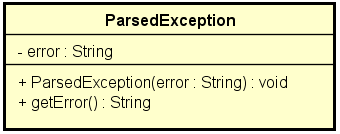
\includegraphics[scale=0.8,keepaspectratio]{img/server/ParsedException.png}}
\caption{\nogloxy{swedesigner::server::project::ParsedException}}
\end{figure}
\FloatBarrier
\begin{itemize}
\item \textbf{Descrizione}\\
Questa classe rappresenta una eccezione che viene sollevata nel momento in cui viene identificata una illegalità nel parsing della stringa in formato .json
\item \textbf{Utilizzo}\\
\texttt{ParsedInterface} solleva un'eccezione nel caso in cui venga identificata una illegalità nel parsing di una interfaccia. Inoltre \texttt{ParsedClass} solleva tale eccezione nel caso venga identificata una illegalità nel parsing di una classe.
\item \textbf{Relazioni con altre classi}:
\begin{itemize}
\item \textit{OUT} \hyperref[\nogloxy{swedesigner::server::project::ParsedClass}]{\nogloxy{\texttt{ParsedClass}}}\\
questa classe estende la classe astratta \texttt{ParsedType}, imponendo al suo interno la presenza di una lista di \texttt{ParsedAttribute}. 
\item \textit{OUT} \hyperref[\nogloxy{swedesigner::server::project::ParsedInterface}]{\nogloxy{\texttt{ParsedInterface}}}\\
questa classe estende la classe astratta \textt{ParsedType} ed ha bisogno soltanto della firma dei metodi essendo una classe che contiene informazioni riguardo un'interfaccia pura.
\end{itemize}
\item \textbf{Attributi}:
\begin{itemize}
\item \nogloxy{\texttt{- error: String}}
\\ Rappresenta la descrizione testuale dell'errore rilevato in fase di parsing.
\end{itemize}
\item \textbf{Metodi}:
\begin{itemize}
\item \nogloxy{\texttt{+ getError(): String}}
\\ Ritorna la descrizione testuale di un errore rilevato in fase di parsing.
\item \nogloxy{\texttt{+ ParsedException(error: String)}}
\\ Costruisce un oggetto ParsedException.
\\ \textbf{Parametri}:
\begin{itemize}
\item \nogloxy{\texttt{error: String}}
\\ Rappresenta il contenuto di un particolare errore.
\end{itemize}
\end{itemize}
\end{itemize}

\subsubsubsection{\nogloxy{swedesigner::server::project::ParsedFor}}
\label{\nogloxy{swedesigner::server::project::ParsedFor}}
\begin{figure}[h]
\centering
\nogloxy{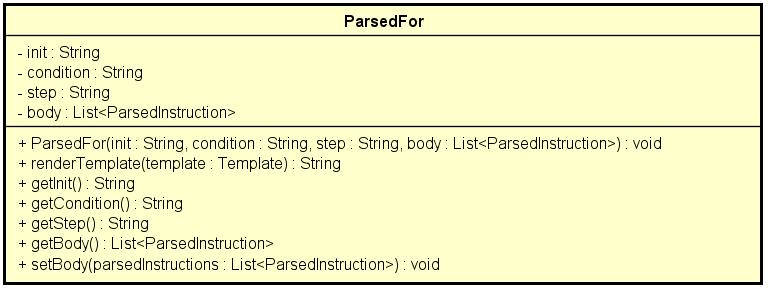
\includegraphics[scale=0.6,keepaspectratio]{img/server/ParsedFor.png}}
\caption{\nogloxy{swedesigner::server::project::ParsedFor}}
\end{figure}
\FloatBarrier
\begin{itemize}
\item \textbf{Descrizione}\\
questa classe descrive il comportamento di un blocco \texttt{for}.
\item \textbf{Utilizzo}\\
dispone della possibilità di effettuare il render di un template in ingresso.
\item \textbf{Classi ereditate}:
\begin{itemize}
\item \hyperref[\nogloxy{swedesigner::server::project::ParsedInstruction}]{\nogloxy{\texttt{ParsedInstruction}}}
\end{itemize}
\item \textbf{Attributi}:
\begin{itemize}
\item \nogloxy{\texttt{- body: List<ParsedInstruction>}}
\\ Indica l'insieme di istruzioni contenute nel corpo del corrispondente oggetto ParsedFor.
\item \nogloxy{\texttt{- condition: String}}
\\ Indica la condizione del corrispondente oggetto ParsedFor.
\item \nogloxy{\texttt{- init: String}}
\\ Indica l'istruzione di inizializzazione del corrispondente oggetto ParsedFor.
\item \nogloxy{\texttt{- step: String}}
\\ Indica il passo di incremento o decremento del corrispondente oggetto ParsedFor.
\end{itemize}
\item \textbf{Metodi}:
\begin{itemize}
\item \nogloxy{\texttt{+ getBody(): List<ParsedInstruction>}}
\\ Ritorna l'insieme di istruzioni contenute nel corpo di un oggetto ParsedFor.
\item \nogloxy{\texttt{+ getCondition(): String}}
\\ Ritorna la condizione di un oggetto ParsedFor.
\item \nogloxy{\texttt{+ getInit(): String}}
\\ Ritorna l'istruzione di inizializzazione dell'oggetto ParsedFor.
\item \nogloxy{\texttt{+ getStep(): String}}
\\ Ritorna il passo di incremento o decremento di un oggetto ParsedFor.
\item \nogloxy{\texttt{+ ParsedFor(init: String, condition: String, step: String)}}
\\ Costruisce un oggetto ParsedFor.
\\ \textbf{Parametri}:
\begin{itemize}
\item \nogloxy{\texttt{init: String}}
\\ Rappresenta l'istruzione di inizializzazione del particolare oggetto ParsedFor che si sta creando.
\item \nogloxy{\texttt{condition: String}}
\\ Rappresenta la condizione del particolare oggetto ParsedFor che si sta creando.

\item \nogloxy{\texttt{step: String}}
\\ Rapprensenta il passo di incremento o decremento del particolare oggetto ParsedFor che si sta creando.
\end{itemize}
\item \nogloxy{\texttt{+ renderTemplate(template: Template): String}}
\\ Traduce l'oggetto ParsedFor in una stringa che rappresenta il codice di un particolare linguaggio di programmazione.
\\ \textbf{Parametri}:
\begin{itemize}
\item \nogloxy{\texttt{template: Template}}
\\ Riferimento alla particolare istanza di Template da utilizzare.
\end{itemize}
\item \nogloxy{\texttt{+ setBody(parsedInstructions: List<ParsedInstruction>): void}}
\\ Permette di assegnare un insieme di istruzioni al corpo di un oggetto ParsedFor.
\\ \textbf{Parametri}:
\begin{itemize}
\item \nogloxy{\texttt{parsedInstructions: List<ParsedInstruction>}}
\\ Rappresenta l'insieme di istruzioni da inserire nel corpo del corrispondente oggetto ParsedFor.
\end{itemize}
\end{itemize}
\end{itemize}

\subsubsubsection{\nogloxy{swedesigner::server::project::ParsedIf}}
\label{\nogloxy{swedesigner::server::project::ParsedIf}}
\begin{figure}[h]
\centering
\nogloxy{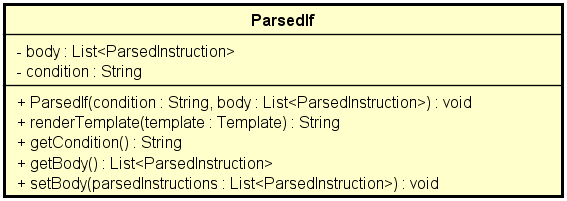
\includegraphics[scale=0.8,keepaspectratio]{img/server/ParsedIf.png}}
\caption{\nogloxy{swedesigner::server::project::ParsedIf}}
\end{figure}
\FloatBarrier
\begin{itemize}
\item \textbf{Descrizione}\\
questa classe descrive il comportamento di un blocco \texttt{if}.
\item \textbf{Utilizzo}\\
dispone della possibilità di effettuare il render di un template in ingresso.
\item \textbf{Classi ereditate}:
\begin{itemize}
\item \hyperref[\nogloxy{swedesigner::server::project::ParsedInstruction}]{\nogloxy{\texttt{ParsedInstruction}}}
\end{itemize}
\item \textbf{Attributi}:
\begin{itemize}
\item \nogloxy{\texttt{- body: List<ParsedInstruction>}}
\\ Indica l'insieme di istruzioni contenute nel corpo del corrispondente oggetto ParsedIf.
\item \nogloxy{\texttt{- condition: String}}
\\ Indica la condizione del corrispondente oggetto ParsedIf.
\end{itemize}
\item \textbf{Metodi}:
\begin{itemize}
\item \nogloxy{\texttt{+ getBody(): List<ParsedInstruction>}}
\\ Ritorna l'insieme di istruzioni contenute nel corpo di un oggetto ParsedIf.
\item \nogloxy{\texttt{+ getCondition(): String}}
\\ Ritorna la condizione di un oggetto ParsedIf.
\item \nogloxy{\texttt{+ ParsedIf(condition: String)}}
\\ Costruisce un oggetto ParsedIf.
\\ \textbf{Parametri}:
\begin{itemize}
\item \nogloxy{\texttt{condition: String}}
\\ Rappresenta la condizione del particolare oggetto ParsedIf che si sta creando.
\end{itemize}
\item \nogloxy{\texttt{+ renderTemplate(template: Template): String}}
\\ Traduce l'oggetto ParsedIf in una stringa che rappresenta il codice di un particolare linguaggio di programmazione.
\\ \textbf{Parametri}:
\begin{itemize}
\item \nogloxy{\texttt{template: Template}}
\\ Riferimento alla particolare istanza di Template da utilizzare.
\end{itemize}
\item \nogloxy{\texttt{+ setBody(parsedInstructions: List<ParsedInstruction>): void}}
\\ Inserisce nel campo dati body del ParsedIf un insieme di ParsedInstruction, ossia inserisce il corpo all'interno del body dell'istruzione \emph{if}.
\\ \textbf{Parametri}:
\begin{itemize}
\item \nogloxy{\texttt{parsedInstructions: List<ParsedInstruction>}}
\\ Indica l'insieme di istruzioni da inserire nel corpo del corrispondente oggetto ParsedIf.
\end{itemize}
\end{itemize}
\end{itemize}

\subsubsubsection{\nogloxy{swedesigner::server::project::ParsedInstruction}}
\label{\nogloxy{swedesigner::server::project::ParsedInstruction}}
\begin{figure}[h]
\centering
\nogloxy{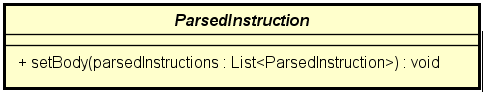
\includegraphics[scale=0.8,keepaspectratio]{img/server/ParsedInstruction.png}}
\caption{\nogloxy{swedesigner::server::project::ParsedInstruction}}
\end{figure}
\FloatBarrier
\begin{itemize}
\item \textbf{Descrizione}\\
questa classe astratta rappresenta la singola istruzione contenuta all'interno di un metodo. Essa è estesa dalle istruzioni specifiche (e.g. \texttt{ParsedIf}, \texttt{ParsedWhile}, etc.)
\item \textbf{Utilizzo}\\
questa classe implementa l'interfaccia \texttt{ParsedElement}.
\item \textbf{Sottoclassi}:
\begin{itemize}
\item \hyperref[\nogloxy{swedesigner::server::project::ParsedCustom}]{\nogloxy{\texttt{ParsedCustom}}}
\item \hyperref[\nogloxy{swedesigner::server::project::ParsedElse}]{\nogloxy{\texttt{ParsedElse}}}
\item \hyperref[\nogloxy{swedesigner::server::project::ParsedFor}]{\nogloxy{\texttt{ParsedFor}}}
\item \hyperref[\nogloxy{swedesigner::server::project::ParsedIf}]{\nogloxy{\texttt{ParsedIf}}}
\item \hyperref[\nogloxy{swedesigner::server::project::ParsedReturn}]{\nogloxy{\texttt{ParsedReturn}}}
\item \hyperref[\nogloxy{swedesigner::server::project::ParsedStatement}]{\nogloxy{\texttt{ParsedStatement}}}
\item \hyperref[\nogloxy{swedesigner::server::project::ParsedWhile}]{\nogloxy{\texttt{ParsedWhile}}}
\end{itemize}
\item \textbf{Relazioni con altre classi}:
\begin{itemize}
\item \textit{IN} \hyperref[\nogloxy{swedesigner::server::project::ParsedMethod}]{\nogloxy{\texttt{ParsedMethod}}}\\
questa classe rappresenta un metodo come insieme di istruzioni \texttt{ParsedIstruction} e un insieme di \texttt{ParsedAttribute} come parametri del metodo.
\item \textit{IN} \hyperref[\nogloxy{swedesigner::server::project::ParsedMethod}]{\nogloxy{\texttt{ParsedMethod}}}\\
questa classe rappresenta un metodo come insieme di istruzioni \texttt{ParsedIstruction} e un insieme di \texttt{ParsedAttribute} come parametri del metodo.
\item \textit{OUT} \hyperref[\nogloxy{swedesigner::server::project::ParsedElement}]{\nogloxy{\texttt{ParsedElement}}}\\
questa classe descrive il contratto di un elemento generico \texttt{Parsed}. Si specifica il metodo \texttt{RenderTemplate} che impone la necessità di implementarlo ad ogni classe sottostante.
\end{itemize}
\item \textbf{Metodi}:
\begin{itemize}
\item \nogloxy{\texttt{+ setBody(parsedInstructions: List<ParsedInstruction>): void}}
\\ Permette di assegnare un insieme di istruzioni al corpo di un oggetto ParsedInstruction.
\\ \textbf{Parametri}:
\begin{itemize}
\item \nogloxy{\texttt{parsedInstructions: List<ParsedInstruction>}}
\\ Rappresenta l'insieme di istruzioni da inserire nel corpo di una particolare ParsedInstruction.
\end{itemize}
\end{itemize}
\end{itemize}

\subsubsubsection{\nogloxy{swedesigner::server::project::ParsedInterface}}
\label{\nogloxy{swedesigner::server::project::ParsedInterface}}
\begin{figure}[h]
\centering
\nogloxy{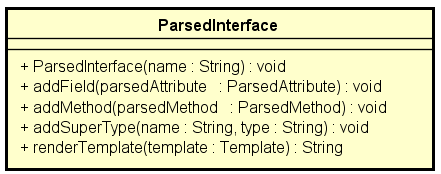
\includegraphics[scale=0.8,keepaspectratio]{img/server/ParsedInterface.png}}
\caption{\nogloxy{swedesigner::server::project::ParsedInterface}}
\end{figure}
\FloatBarrier
\begin{itemize}
\item \textbf{Descrizione}\\
questa classe estende la classe astratta \textt{ParsedType} ed ha bisogno soltanto della firma dei metodi essendo una classe che contiene informazioni riguardo un'interfaccia pura.
\item \textbf{Utilizzo}\\
questa classe è creata tramite la \texttt{ElementFactory} durante il parsing del progetto e inserita all'interno di \texttt{ParsedProgram}.
\item \textbf{Classi ereditate}:
\begin{itemize}
\item \hyperref[\nogloxy{swedesigner::server::project::ParsedType}]{\nogloxy{\texttt{ParsedType}}}
\end{itemize}
\item \textbf{Relazioni con altre classi}:
\begin{itemize}
\item \textit{IN} \hyperref[\nogloxy{swedesigner::server::project::ParsedException}]{\nogloxy{\texttt{ParsedException}}}\\
Questa classe rappresenta una eccezione che viene sollevata nel momento in cui viene identificata una illegalità nel parsing della stringa in formato .json
\item \textit{OUT} \hyperref[\nogloxy{swedesigner::server::project::ParsedMethod}]{\nogloxy{\texttt{ParsedMethod}}}\\
questa classe rappresenta un metodo come insieme di istruzioni \texttt{ParsedIstruction} e un insieme di \texttt{ParsedAttribute} come parametri del metodo.
\end{itemize}
\item \textbf{Metodi}:
\begin{itemize}
\item \nogloxy{\texttt{+ addField(parsedAttribute: ParsedAttribute): void}}
\\ Aggiunge all'oggetto ParsedInterface un campo dati rappresentato da un oggetto ParsedAttribute.
\\ \textbf{Parametri}:
\begin{itemize}
\item \nogloxy{\texttt{parsedAttribute: ParsedAttribute}}
\\ Rappresenta un campo dati in forma di oggetto ParsedAttribute.
\end{itemize}
\item \nogloxy{\texttt{+ addMethod(parsedMethod: ParsedMethod): void}}
\\ Aggiunge ad un oggetto ParsedInterface un metodo rappresentato da un oggetto ParsedMethod.
\\ \textbf{Parametri}:
\begin{itemize}
\item \nogloxy{\texttt{parsedMethod: ParsedMethod}}
\\ Rappresenta un metodo in forma di oggetto ParsedMethod.
\end{itemize}
\item \nogloxy{\texttt{+ addSupertype(name: String, type: String): void}}
\\ Aggiunge il nome di uno dei "supertipi" diretti dell'oggetto ParsedInterface.
\\ \textbf{Parametri}:
\begin{itemize}
\item \nogloxy{\texttt{name: String}}
\\ Rappresenta il nome del "supertipo" che deve essere esteso.
\item \nogloxy{\texttt{type: String}}
\\ Indica il supertipo tipo che deve essere esteso.
\end{itemize}
\item \nogloxy{\texttt{+ ParsedInterface(name: String)}}
\\ Costruisce un oggetto ParsedInterface.
\\ \textbf{Parametri}:
\begin{itemize}
\item \nogloxy{\texttt{name: String}}
\\ Rappresenta il nome del particolare oggetto ParsedInterface che si sta creando.
\end{itemize}
\item \nogloxy{\texttt{+ renderTemplate(template: Template): String}}
\\ Traduce l'oggetto ParsedInterface in una stringa che rappresenta il codice di un particolare linguaggio di programmazione.
\\ \textbf{Parametri}:
\begin{itemize}
\item \nogloxy{\texttt{template: Template}}
\\ Riferimento alla particolare istanza di Template da utilizzare.
\end{itemize}
\end{itemize}
\end{itemize}

\subsubsubsection{\nogloxy{swedesigner::server::project::ParsedMethod}}
\label{\nogloxy{swedesigner::server::project::ParsedMethod}}
\begin{figure}[h]
\centering
\nogloxy{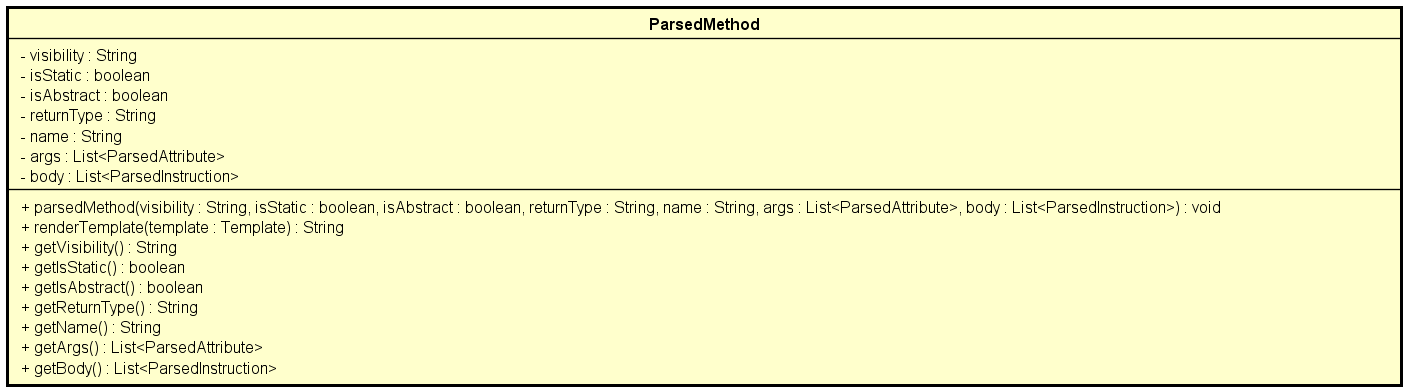
\includegraphics[scale=0.5,keepaspectratio]{img/server/ParsedMethod.png}}
\caption{\nogloxy{swedesigner::server::project::ParsedMethod}}
\end{figure}
\FloatBarrier
\begin{itemize}
\item \textbf{Descrizione}\\
questa classe rappresenta un metodo come insieme di istruzioni \texttt{ParsedIstruction} e un insieme di \texttt{ParsedAttribute} come parametri del metodo.
\item \textbf{Utilizzo}\\
questa classe è usata da \texttt{ParsedType} come descritto in precedenza. La classe inoltre implementa l'interfaccia \texttt{ParsedElement}.
\item \textbf{Classi ereditate}:
\begin{itemize}
\item \hyperref[\nogloxy{swedesigner::server::project::ParsedElement}]{\nogloxy{\texttt{ParsedElement}}}
\end{itemize}
\item \textbf{Relazioni con altre classi}:
\begin{itemize}
\item \textit{IN} \hyperref[\nogloxy{swedesigner::server::project::ParsedClass}]{\nogloxy{\texttt{ParsedClass}}}\\
questa classe estende la classe astratta \texttt{ParsedType}, imponendo al suo interno la presenza di una lista di \texttt{ParsedAttribute}. 
\item \textit{IN} \hyperref[\nogloxy{swedesigner::server::project::ParsedInterface}]{\nogloxy{\texttt{ParsedInterface}}}\\
questa classe estende la classe astratta \textt{ParsedType} ed ha bisogno soltanto della firma dei metodi essendo una classe che contiene informazioni riguardo un'interfaccia pura.
\item \textit{IN} \hyperref[\nogloxy{swedesigner::server::project::ParsedType}]{\nogloxy{\texttt{ParsedType}}}\\
questa classe astratta definisce un contratto comune tra le classi \texttt{ParsedInterface} e \texttt{ParsedClass}. 
\item \textit{OUT} \hyperref[\nogloxy{swedesigner::server::project::ParsedAttribute}]{\nogloxy{\texttt{ParsedAttribute}}}\\
questa classe rappresenta un singolo attributo, memorizzando il nome della variabile, la sua visibilità e il suo valore di default. Viene utilizzata anche per rappresentare i parametri dei metodi.
% Tuttavia, ciò non vale per attributi statici. 
% Nella \emph{Definizione_di_prodotto_v_1_0_0} [RIFERIMENTO] sarà esplicitata l'implementazione di dettaglio decisa.
\item \textit{OUT} \hyperref[\nogloxy{swedesigner::server::project::ParsedAttribute}]{\nogloxy{\texttt{ParsedAttribute}}}\\
questa classe rappresenta un singolo attributo, memorizzando il nome della variabile, la sua visibilità e il suo valore di default. Viene utilizzata anche per rappresentare i parametri dei metodi.
% Tuttavia, ciò non vale per attributi statici. 
% Nella \emph{Definizione_di_prodotto_v_1_0_0} [RIFERIMENTO] sarà esplicitata l'implementazione di dettaglio decisa.
\item \textit{OUT} \hyperref[\nogloxy{swedesigner::server::project::ParsedElement}]{\nogloxy{\texttt{ParsedElement}}}\\
questa classe descrive il contratto di un elemento generico \texttt{Parsed}. Si specifica il metodo \texttt{RenderTemplate} che impone la necessità di implementarlo ad ogni classe sottostante.
\item \textit{OUT} \hyperref[\nogloxy{swedesigner::server::project::ParsedElement}]{\nogloxy{\texttt{ParsedElement}}}\\
questa classe descrive il contratto di un elemento generico \texttt{Parsed}. Si specifica il metodo \texttt{RenderTemplate} che impone la necessità di implementarlo ad ogni classe sottostante.
\item \textit{OUT} \hyperref[\nogloxy{swedesigner::server::project::ParsedInstruction}]{\nogloxy{\texttt{ParsedInstruction}}}\\
questa classe astratta rappresenta la singola istruzione contenuta all'interno di un metodo. Essa è estesa dalle istruzioni specifiche (e.g. \texttt{ParsedIf}, \texttt{ParsedWhile}, etc.)
\item \textit{OUT} \hyperref[\nogloxy{swedesigner::server::project::ParsedInstruction}]{\nogloxy{\texttt{ParsedInstruction}}}\\
questa classe astratta rappresenta la singola istruzione contenuta all'interno di un metodo. Essa è estesa dalle istruzioni specifiche (e.g. \texttt{ParsedIf}, \texttt{ParsedWhile}, etc.)
\end{itemize}
\item \textbf{Attributi}:
\begin{itemize}
\item \nogloxy{\texttt{- args: List<ParsedAttribute>}}
\\ Indica l'insieme di ParsedAttribute che rappresentano i parametri di un ParsedMethod.
\item \nogloxy{\texttt{- body: List<ParsedInstruction>}}
\\ Indica l'insieme di istruzioni che compongono il corpo del relativo oggetto ParsedMethod.
\item \nogloxy{\texttt{- isAbstract: boolean}}
\\ Indica se il ParsedMethod rappresenta un metodo astratto o meno.
\item \nogloxy{\texttt{- isStatic: boolean}}
\\ Indica se il ParsedMethod rappresenta un metodo statico o meno.
\item \nogloxy{\texttt{- name: String}}
\\ Indica il nome dell'oggetto ParsedMethod.
\item \nogloxy{\texttt{- returnType: String}}
\\ Indica il tipo di ritorno di un oggetto ParsedMethod.
\item \nogloxy{\texttt{- visibility: String}}
\\ Indica la visibilità dell'oggetto ParsedMethod.
\end{itemize}
\item \textbf{Metodi}:
\begin{itemize}
\item \nogloxy{\texttt{+ getArgs(): List<ParsedAttribute>}}
\\ Ritorna l'insieme di ParsedAttribute che rappresentano i parametri di un ParsedMethod.
\item \nogloxy{\texttt{+ getBody(): List<ParsedInstruction>}}
\\ Ritorna l'insieme di istruzioni che compongono il corpo del relativo oggetto ParsedMethod.
\item \nogloxy{\texttt{+ getIsAbstract(): boolean}}
\\ Indica se l'oggetto ParsedMethod è astratto o meno.
\item \nogloxy{\texttt{+ getIsStatic(): boolean}}
\\ Ritorna informazioni riguardanti la staticità di un oggetto ParsedMethod.
\item \nogloxy{\texttt{+ getName(): String}}
\\ Ritorna il nome di un oggetto ParsedMethod.
\item \nogloxy{\texttt{+ getReturnType(): String}}
\\ Ritorna il tipo di ritorno di un oggetto ParsedMethod.
\item \nogloxy{\texttt{+ getVisibility(): String}}
\\ Ritorna la visibilità di un oggetto ParsedMethod.
\item \nogloxy{\texttt{+ ParsedMethod(visibility: String, isStatic: boolean, isAbstract: boolean, returnType: String, args: List<ParsedAttribute>, body: List<ParsedInstruction>, name: String)}}
\\ Costruisce un oggetto ParsedMethod.
\\ \textbf{Parametri}:
\begin{itemize}
\item \nogloxy{\texttt{visibility: String}}
\\ Rappresenta la visibilità dell'oggetto ParsedMethod che si sta creando.
\item \nogloxy{\texttt{isStatic: boolean}}
\\ Indica se il ParsedMethod che si sta creando rappresenterà un metodo statico o meno.
\item \nogloxy{\texttt{isAbstract: boolean}}
\\ Indica se il ParsedMethod che si sta creando rappresenterà un metodo astratto o meno.
\item \nogloxy{\texttt{returnType: String}}
\\ Indica il tipo di ritorno dell'oggetto ParsedMethod che si sta creando.
\item \nogloxy{\texttt{args: List<ParsedAttribute>}}
\\ Indica l'insieme di ParsedAttribute che rappresenteranno i parametri del ParsedMethod che si sta creando.
\item \nogloxy{\texttt{body: List<ParsedInstruction>}}
\\ Indica l'insieme di istruzioni che comporranno il corpo del relativo oggetto ParsedMethod che si sta creando.
\item \nogloxy{\texttt{name: String}}
\\ Indica il nome dell'oggetto ParsedMethod che si sta creando.
\end{itemize}
\item \nogloxy{\texttt{+ renderTemplate(template: Tempate): String}}
\\ Traduce l'oggetto ParsedMethod in una stringa che rappresenta il codice di un particolare linguaggio di programmazione.
\\ \textbf{Parametri}:
\begin{itemize}
\item \nogloxy{\texttt{template: Tempate}}
\\ Riferimento alla particolare istanza di Template da utilizzare.
\end{itemize}
\end{itemize}
\end{itemize}

\subsubsubsection{\nogloxy{swedesigner::server::project::ParsedProgram}}
\label{\nogloxy{swedesigner::server::project::ParsedProgram}}
\begin{figure}[h]
\centering
\nogloxy{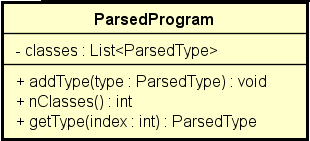
\includegraphics[scale=0.8,keepaspectratio]{img/server/ParsedProgram.png}}
\caption{\nogloxy{swedesigner::server::project::ParsedProgram}}
\end{figure}
\FloatBarrier
\begin{itemize}
\item \textbf{Descrizione}\\
questa classe rappresenta l'entità che possiede al suo interno tutte le componenti di un progetto. Essa possiede più \texttt{ParsedType}.
\item \textbf{Utilizzo}\\
La classe \texttt{Parser} ha una dipendenza verso questo elemento: essa infatti ne crea una e la ritorna al controller, il quale la passerà alla classe \texttt{Generator}.
\item \textbf{Relazioni con altre classi}:
\begin{itemize}
\item \textit{IN} \hyperref[\nogloxy{swedesigner::server::parser::Parser}]{\nogloxy{\texttt{Parser}}}\\
questa classe si occupa di elaborare il file JSON proveniente dal client e di creare da esso un oggetto Java \texttt{ParsedProgram} strutturato in modo da poter essere facilmente convertito in codice.
\item \textit{OUT} \hyperref[\nogloxy{swedesigner::server::project::ParsedType}]{\nogloxy{\texttt{ParsedType}}}\\
questa classe astratta definisce un contratto comune tra le classi \texttt{ParsedInterface} e \texttt{ParsedClass}. 
\end{itemize}
\item \textbf{Attributi}:
\begin{itemize}
\item \nogloxy{\texttt{- classes: List<ParsedType>}}
\\ Indica l'insieme di classi ed interfacce, sottoforma di ParsedClass e ParsedInterface, che formano un ParsedProgram.
\end{itemize}
\item \textbf{Metodi}:
\begin{itemize}
\item \nogloxy{\texttt{+ addType(type: ParsedType): void}}
\\ Aggiunge un tipo (ParsedClass o ParsedInterface) al ParsedProgram, ossia aggiunge una classe o un'interfaccia al programma.
\\ \textbf{Parametri}:
\begin{itemize}
\item \nogloxy{\texttt{type: ParsedType}}
\\ Rappresenta un ParsedType (ParsedClass o ParsedInterface) che deve essere inserito nel particolare ParsedProgram, ossia la classe o l'nterfaccia da aggiungere al programma.
\end{itemize}
\item \nogloxy{\texttt{+ getType(position: int): ParsedType}}
\\ Ritorna l'i-esimo elemento (ParsedClass o ParsedInterface) contenuto nella lista di ParsedType.
\\ \textbf{Parametri}:
\begin{itemize}
\item \nogloxy{\texttt{position: int}}
\\ Rappresenta la posizione di un particolare ParsedType all'interno del ParsedProgram.
\end{itemize}
\item \nogloxy{\texttt{+ numberClasses(): int}}
\\ Ritorna il numero complessivo di classi ed interfacce che formano il ParsedProgram.
\end{itemize}
\end{itemize}

\subsubsubsection{\nogloxy{swedesigner::server::project::ParsedReturn}}
\label{\nogloxy{swedesigner::server::project::ParsedReturn}}
\begin{figure}[h]
\centering
\nogloxy{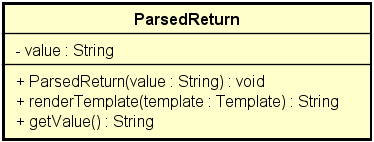
\includegraphics[scale=0.8,keepaspectratio]{img/server/ParsedReturn.png}}
\caption{\nogloxy{swedesigner::server::project::ParsedReturn}}
\end{figure}
\FloatBarrier
\begin{itemize}
\item \textbf{Descrizione}\\
questa classe descrive il comportamento di un blocco di ritorno di un metodo.
\item \textbf{Utilizzo}\\
dispone della possibilità di effettuare il render di un template in ingresso.
\item \textbf{Classi ereditate}:
\begin{itemize}
\item \hyperref[\nogloxy{swedesigner::server::project::ParsedInstruction}]{\nogloxy{\texttt{ParsedInstruction}}}
\end{itemize}
\item \textbf{Attributi}:
\begin{itemize}
\item \nogloxy{\texttt{- value: String}}
\\ Rappresenta il valore di un oggetto ParsedReturn, ossia ciò che viene ritornato da un metodo.
\end{itemize}
\item \textbf{Metodi}:
\begin{itemize}
\item \nogloxy{\texttt{+ getValue(): String}}
\\ Ritorna il valore del corrispondente oggetto ParsedReturn.
\item \nogloxy{\texttt{+ ParsedReturn(value: String)}}
\\ Costruisce un oggetto ParsedReturn.
\\ \textbf{Parametri}:
\begin{itemize}
\item \nogloxy{\texttt{value: String}}
\\ Rappresenta il valore che dovrà essere assegnato al campo dati value di un oggetto ParsedReturn.
\end{itemize}
\item \nogloxy{\texttt{+ renderTemplate(template: Template): String}}
\\ Traduce l'oggetto ParsedReturn in una stringa che rappresenta il codice di un particolare linguaggio di programmazione.
\\ \textbf{Parametri}:
\begin{itemize}
\item \nogloxy{\texttt{template: Template}}
\\ Riferimento alla particolare istanza di Template da utilizzare.
\end{itemize}
\end{itemize}
\end{itemize}

\subsubsubsection{\nogloxy{swedesigner::server::project::ParsedStatement}}
\label{\nogloxy{swedesigner::server::project::ParsedStatement}}
\begin{figure}[h]
\centering
\nogloxy{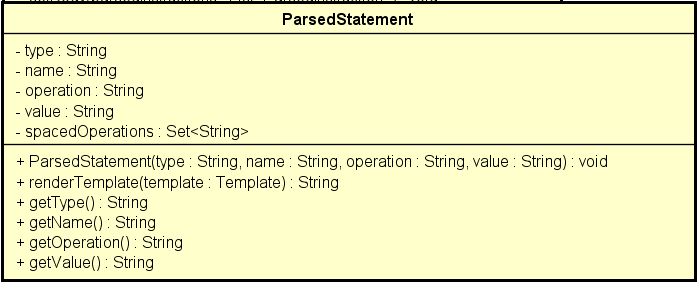
\includegraphics[scale=0.8,keepaspectratio]{img/server/ParsedStatement.png}}
\caption{\nogloxy{swedesigner::server::project::ParsedStatement}}
\end{figure}
\FloatBarrier
\begin{itemize}
\item \textbf{Descrizione}\\
questa classe descrive il comportamento di un blocco di assegnazione variabile o inizializzazione variabile.	
\item \textbf{Utilizzo}\\
dispone della possibilità di effettuare il render di un template in ingresso.
\item \textbf{Classi ereditate}:
\begin{itemize}
\item \hyperref[\nogloxy{swedesigner::server::project::ParsedInstruction}]{\nogloxy{\texttt{ParsedInstruction}}}
\end{itemize}
\item \textbf{Attributi}:
\begin{itemize}
\item \nogloxy{\texttt{- name: String}}
\\ Indica il nome dell'oggetto ParsedStatement.
\item \nogloxy{\texttt{- operation: String}}
\\ Indica l'operazione dell'oggetto ParsedStatement.
\item \nogloxy{\texttt{- spacedOperation: Set<String>}}
\\ Indica l'insieme di operatori legali utilizzabili nello statement.
\item \nogloxy{\texttt{- type: String}}
\\ Indica il tipo dell'oggetto ParsedStatement.
\item \nogloxy{\texttt{- value: String}}
\\ Indica il valore dell'oggetto ParsedStatement.
\end{itemize}
\item \textbf{Metodi}:
\begin{itemize}
\item \nogloxy{\texttt{+ getName(): String}}
\\ Ritorna il nome dell'oggetto ParsedStatement.
\item \nogloxy{\texttt{+ getOperation(): String}}
\\ Ritorna l'operatore dell'oggetto ParsedStatement.
\item \nogloxy{\texttt{+ getType(): String}}
\\ Ritorna il tipo dell'oggetto ParsedStatement.
\item \nogloxy{\texttt{+ getValue(): String}}
\\ Ritorna il valore dell'oggetto ParsedStatement.
\item \nogloxy{\texttt{+ ParsedStatment(type: String, name: String, operation: String, value: String)}}
\\ Costruisce un oggetto ParsedStatement.
\\ \textbf{Parametri}:
\begin{itemize}
\item \nogloxy{\texttt{type: String}}
\\ Rappresenta il tipo dell'oggetto ParsedStatement che si sta creando.
\item \nogloxy{\texttt{name: String}}
\\ Rappresenta il nome dell'oggetto ParsedStatement che si sta creando.
\item \nogloxy{\texttt{operation: String}}
\\ Rappresenta l'operazione dell'oggetto ParsedStatement che si sta creando.
\item \nogloxy{\texttt{value: String}}
\\ Indica il valore dell'oggetto ParsedStatement che si sta creando.
\end{itemize}
\item \nogloxy{\texttt{+ renderTemplate(template: Template): String}}
\\ Traduce l'oggetto ParsedStatement in una stringa che rappresenta il codice di un particolare linguaggio di programmazione.
\\ \textbf{Parametri}:
\begin{itemize}
\item \nogloxy{\texttt{template: Template}}
\\ Riferimento alla particolare istanza di Template da utilizzare.
\end{itemize}
\end{itemize}
\end{itemize}

\subsubsubsection{\nogloxy{swedesigner::server::project::ParsedType}}
\label{\nogloxy{swedesigner::server::project::ParsedType}}
\begin{figure}[h]
\centering
\nogloxy{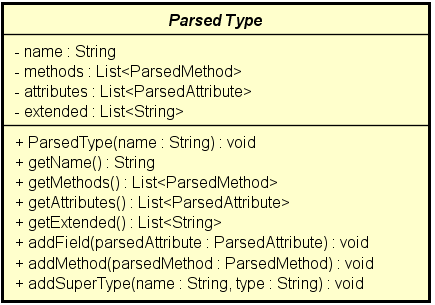
\includegraphics[scale=0.8,keepaspectratio]{img/server/ParsedType.png}}
\caption{\nogloxy{swedesigner::server::project::ParsedType}}
\end{figure}
\FloatBarrier
\begin{itemize}
\item \textbf{Descrizione}\\
questa classe astratta definisce un contratto comune tra le classi \texttt{ParsedInterface} e \texttt{ParsedClass}. 
\item \textbf{Utilizzo}\\
essa possiede un insieme di \texttt{ParsedMethod}. Nell'accezione di molti linguaggi, classi e interfacce rappresentano dei tipi. Questa classe deriva da \texttt{ParsedElement} al fine di poter usare polimorfismo sugli elementi creati dal \texttt{Parser}. 
I tipi sono creati dalla \texttt{ParsedFactory} e sono richiesti da \texttt{Parser}.
\item \textbf{Sottoclassi}:
\begin{itemize}
\item \hyperref[\nogloxy{swedesigner::server::project::ParsedClass}]{\nogloxy{\texttt{ParsedClass}}}
\item \hyperref[\nogloxy{swedesigner::server::project::ParsedInterface}]{\nogloxy{\texttt{ParsedInterface}}}
\end{itemize}
\item \textbf{Relazioni con altre classi}:
\begin{itemize}
\item \textit{IN} \hyperref[\nogloxy{swedesigner::server::project::ParsedProgram}]{\nogloxy{\texttt{ParsedProgram}}}\\
questa classe rappresenta l'entità che possiede al suo interno tutte le componenti di un progetto. Essa possiede più \texttt{ParsedType}.
\item \textit{OUT} \hyperref[\nogloxy{swedesigner::server::project::ParsedElement}]{\nogloxy{\texttt{ParsedElement}}}\\
questa classe descrive il contratto di un elemento generico \texttt{Parsed}. Si specifica il metodo \texttt{RenderTemplate} che impone la necessità di implementarlo ad ogni classe sottostante.
\item \textit{OUT} \hyperref[\nogloxy{swedesigner::server::project::ParsedMethod}]{\nogloxy{\texttt{ParsedMethod}}}\\
questa classe rappresenta un metodo come insieme di istruzioni \texttt{ParsedIstruction} e un insieme di \texttt{ParsedAttribute} come parametri del metodo.
\end{itemize}
\item \textbf{Attributi}:
\begin{itemize}
\item \nogloxy{\texttt{- attributes: List<ParsedAttribute>}}
\\ Rappresenta la lista dei campi dati di un particolare ParsedType.
\item \nogloxy{\texttt{- extended: List<String>}}
\\ Rappresenta l'insieme dei "supertipi" diretti estesi da un particolare ParsedType.
\item \nogloxy{\texttt{- methods: List<ParsedMethod>}}
\\ Rappresenta la lista dei metodi di un particolare ParsedType.
\item \nogloxy{\texttt{- name: String}}
\\ Rappresenta il nome di un particolare oggetto ParsedType.
\end{itemize}
\item \textbf{Metodi}:
\begin{itemize}
\item \nogloxy{\texttt{+ addField(parsedAttribute: ParsedAttribute): void}}
\\ Aggiunge all'oggetto ParsedType un campo dati rappresentato da un oggetto ParsedAttribute.
\\ \textbf{Parametri}:
\begin{itemize}
\item \nogloxy{\texttt{parsedAttribute: ParsedAttribute}}
\\ Rappresenta il campo dati da inserire in un particolare oggetto ParsedType.
\end{itemize}
\item \nogloxy{\texttt{+ addMethod(parsedMethod: ParsedMethod): void}}
\\ Aggiunge ad un oggetto ParsedType un metodo rappresentato da un oggetto ParsedMethod.
\\ \textbf{Parametri}:
\begin{itemize}
\item \nogloxy{\texttt{parsedMethod: ParsedMethod}}
\\ Rappresenta il metodo da inserire in un particolare ParsedType.
\end{itemize}
\item \nogloxy{\texttt{+ addSupertype(name: String, type: String): void}}
\\ Aggiunge il nome di uno dei "supertipi" diretti dell'oggetto ParsedType.
\\ \textbf{Parametri}:
\begin{itemize}
\item \nogloxy{\texttt{name: String}}
\\ Indica il nome del "supertipo" che deve essere implementato o esteso.
\item \nogloxy{\texttt{type: String}}
\\ Indica il tipo, classe o interfaccia, che deve essere rispettivamente esteso o implementato.
\end{itemize}
\item \nogloxy{\texttt{+ getAttributes(): List<ParsedAttribute>}}
\\ Ritorna la lista di campi dati di un particolare ParsedType.
\item \nogloxy{\texttt{+ getExtended(): List<String>}}
\\ Ritorna la lista dei supertipi diretti estesi da un particolare ParsedType.
\item \nogloxy{\texttt{+ getMethods(): List<ParsedMethod>}}
\\ Ritorna la lista dei metodi di un particolare ParsedType.
\item \nogloxy{\texttt{+ getName(): String}}
\\ Ritorna il nome di un particolare ParsedType.
\item \nogloxy{\texttt{+ ParsedType(name: String)}}
\\ Costruisce un oggetto ParsedType.
\\ \textbf{Parametri}:
\begin{itemize}
\item \nogloxy{\texttt{name: String}}
\\ Rappresenta il nome dell'oggetto ParsedType che si sta creando.
\end{itemize}
\end{itemize}
\end{itemize}

\subsubsubsection{\nogloxy{swedesigner::server::project::ParsedWhile}}
\label{\nogloxy{swedesigner::server::project::ParsedWhile}}
\begin{figure}[h]
\centering
\nogloxy{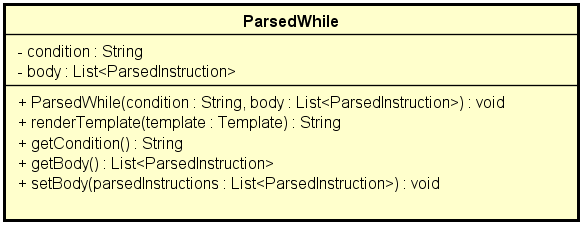
\includegraphics[scale=0.8,keepaspectratio]{img/server/ParsedWhile.png}}
\caption{\nogloxy{swedesigner::server::project::ParsedWhile}}
\end{figure}
\FloatBarrier
\begin{itemize}
\item \textbf{Descrizione}\\
questa classe descrive il comportamento di un blocco \texttt{while} e dispone della possibilità di effettuare il render di un template in ingresso.
\item \textbf{Utilizzo}\\
deriva da \texttt{ParsedInstruction}.
\item \textbf{Classi ereditate}:
\begin{itemize}
\item \hyperref[\nogloxy{swedesigner::server::project::ParsedInstruction}]{\nogloxy{\texttt{ParsedInstruction}}}
\end{itemize}
\item \textbf{Attributi}:
\begin{itemize}
\item \nogloxy{\texttt{- body: List<String>}}
\\ Indica l'insieme di istruzioni contenute nel corpo del corrispondente oggetto ParsedWhile.
\item \nogloxy{\texttt{- condition: String}}
\\ Indica la condizione del corrispondente oggetto ParsedWhile.
\end{itemize}
\item \textbf{Metodi}:
\begin{itemize}
\item \nogloxy{\texttt{+ getBody(): List<ParsedInstruction>}}
\\ Ritorna l'insieme di istruzioni contenute nel corpo di un oggetto ParsedWhile.
\item \nogloxy{\texttt{+ getCondition(): String}}
\\ Ritorna la condizione di un oggetto ParsedWhile.
\item \nogloxy{\texttt{+ ParsedWhile(condition: String, body: List<ParsedInstruction>)}}
\\ Costruisce un oggetto ParsedWhile.
\\ \textbf{Parametri}:
\begin{itemize}
\item \nogloxy{\texttt{condition: String}}
\\ Rappresenta la condizione dell'oggetto ParsedWhile che si sta creando.
\item \nogloxy{\texttt{body: List<ParsedInstruction>}}
\\ Rappresenta l'insieme di istruzioni contenute nel corpo dell'oggetto ParsedWhile che si sta creando.
\end{itemize}
\item \nogloxy{\texttt{+ renderTemplate(template: Template): String}}
\\ Traduce l'oggetto ParsedWhile in una stringa che rappresenta il codice di un particolare linguaggio di programmazione.
\\ \textbf{Parametri}:
\begin{itemize}
\item \nogloxy{\texttt{template: Template}}
\\ Riferimento alla particolare istanza di Template da utilizzare.
\end{itemize}
\item \nogloxy{\texttt{+ setBody(parsedInstructions: List<ParsedInstruction>): void}}
\\ Permette di assegnare un insieme di istruzioni al corpo di un oggetto ParsedWhile.
\\ \textbf{Parametri}:
\begin{itemize}
\item \nogloxy{\texttt{parsedInstructions: List<ParsedInstruction>}}
\\ Rappresenta l'insieme di istruzioni da inserire nel corpo del corrispondente oggetto ParsedWhile.
\end{itemize}
\end{itemize}
\end{itemize}
\subsection{\nogloxy{swedesigner::server::stereotype}}
\label{\nogloxy{swedesigner::server::stereotype}}
\subsubsection{Informazioni generali}
\begin{itemize}
\item \textbf{Descrizione}\\
Questo package offre le classi che descrivono ciò che caratterizza un particolare stereotipo. Queste classi derivano tutte da una classe base chiamata \texttt{Stereotype}. Le classi che definiscono come deve variare ogni stereotipo sono contraddistinte dal suffisso \texttt{Stereotype} (e.g. \texttt{BoardStereotype}). Si noti che tra queste classi non sono presenti dei legami, in quanto sono necessarie alla generazione del codice. La struttura degli stereotipi assegnabili ad ogni classe e le loro relazioni saranno definite successivamente nella \emph{Definizione di Prodotto}.
\item \textbf{Padre}: \hyperref[\nogloxy{swedesigner::server}]{\nogloxy{\texttt{server}}}
\end{itemize}

\subsection{\nogloxy{swedesigner::server::template}}
\label{\nogloxy{swedesigner::server::template}}
\subsubsection{Informazioni generali}
\begin{itemize}
\item \textbf{Descrizione}\\
Questo package contiene le classi necessarie a trasformare l'oggetto che rappresenta il programma in una stringa di testo che rappresenta il codice sorgente tramite un sistema a template, il quale definirà tramite dei file di testo la struttura di ogni componente del programma; per facilitare questo compito sarà usata la libreria \stringtemplate{}. Similarmente al package \texttt{Generator} si è prevista la possibilità di implementare un sistema di template per ogni linguaggio, implementando diversamente l'interfaccia della classe Template e definendo un nuovo package (e.g. \texttt{Java}).
\item \textbf{Padre}: \hyperref[\nogloxy{swedesigner::server}]{\nogloxy{\texttt{server}}}
\item \textbf{Package contenuti}:
\begin{itemize}
\item \hyperref[\nogloxy{swedesigner::server::template::java}]{\nogloxy{\texttt{java}}}\\
Questo package definisce le operazioni necessarie all'applicazione del template relativo al linguaggio Java. Simili package possono essere creati per permettere l'esportazione in diversi linguaggi target.
\end{itemize}
\end{itemize}
\subsubsection{Classi}
\subsubsubsection{\nogloxy{swedesigner::server::template::Template}}
\label{\nogloxy{swedesigner::server::template::Template}}
\begin{figure}[h]
\centering
\nogloxy{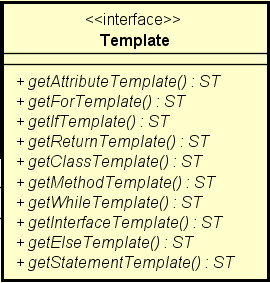
\includegraphics[scale=0.8,keepaspectratio]{img/server/Template.png}}
\caption{\nogloxy{swedesigner::server::template::Template}}
\end{figure}
\FloatBarrier
\begin{itemize}
\item \textbf{Descrizione}\\
questa interfaccia si occupa di fornire un oggetto template generico a chi lo richiede in modo da poter rendere estensibile il sistema aggiungendo un'implementazione concreta del template del linguaggio target desiderato.
\item \textbf{Utilizzo}\\
\texttt{RequestHandlerController} ha una dipendenza verso Template in quanto chiederà a \texttt{TemplateAssembler} una implementazione concreta di un \texttt{Template} in base al linguaggio target. Il pattern realizzato con questa classe è una \emph{dependency injection}.
\item \textbf{Relazioni con altre classi}:
\begin{itemize}
\item \textit{IN} \hyperref[\nogloxy{swedesigner::server::generator::Generator}]{\nogloxy{\texttt{Generator}}}\\
questa interfaccia si occupa di fornire un oggetto \texttt{Generator} generico a chi lo richiede in modo da poter rendere entensibile il sistema aggiungendo un'implementazione concreta del generator del linguaggio target desiderato.
\item \textit{IN} \hyperref[\nogloxy{swedesigner::server::template::java::JavaTemplate}]{\nogloxy{\texttt{JavaTemplate}}}\\
questa classe è una implementazione di \texttt{Template} che permette di fornire un template di una classe, metodo o costrutto Java.
\end{itemize}
\item \textbf{Metodi}:
\begin{itemize}
\item \nogloxy{\texttt{+ getAttributeTemplate(): ST}}
\\ Ritorna il template per tradurre un oggetto ParsedAttribute nel codice di un particolare linguaggio.
\item \nogloxy{\texttt{+ getClassTemplate(): ST}}
\\ Ritorna il template per tradurre un oggetto ParsedClass nel codice di un particolare linguaggio.
\item \nogloxy{\texttt{+ getElseTemplate(): ST}}
\\ Ritorna il template per tradurre un oggetto ParsedElse nel codice di un particolare linguaggio.
\item \nogloxy{\texttt{+ getForTemplate(): ST}}
\\ Ritorna il template per tradurre un oggetto ParsedFor nel codice di un particolare linguaggio.
\item \nogloxy{\texttt{+ getIfTemplate(): ST}}
\\ Ritorna il template per tradurre un oggetto ParsedIf nel codice di un particolare linguaggio.
\item \nogloxy{\texttt{+ getInterfaceTemplate(): ST}}
\\ Ritorna il template per tradurre un oggetto ParsedInterface nel codice di un particolare linguaggio.
\item \nogloxy{\texttt{+ getMethodTemplate(): ST}}
\\ Ritorna il template per tradurre un oggetto ParsedMethod nel codice di un particolare linguaggio.
\item \nogloxy{\texttt{+ getReturnTemplate(): ST}}
\\ Ritorna il template per tradurre un oggetto ParsedReturn nel codice di un particolare linguaggio.
\item \nogloxy{\texttt{+ getStatementTemplate(): ST}}
\\ Ritorna il template per tradurre un oggetto ParsedStatement nel codice di un particolare linguaggio.
\item \nogloxy{\texttt{+ getWhileTemplate(): ST}}
\\ Ritorna il template per tradurre un oggetto ParsedWhile nel codice di un particolare linguaggio.
\end{itemize}
\end{itemize}
\subsection{\nogloxy{swedesigner::server::template::java}}
\label{\nogloxy{swedesigner::server::template::java}}
\subsubsection{Informazioni generali}
\begin{itemize}
\item \textbf{Descrizione}\\
Questo package definisce le operazioni necessarie all'applicazione del template relativo al linguaggio Java. Simili package possono essere creati per permettere l'esportazione in diversi linguaggi target.
\item \textbf{Padre}: \hyperref[\nogloxy{swedesigner::server::template}]{\nogloxy{\texttt{template}}}
\end{itemize}
\subsubsection{Classi}
\subsubsubsection{\nogloxy{swedesigner::server::template::java::JavaTemplate}}
\label{\nogloxy{swedesigner::server::template::java::JavaTemplate}}
\begin{figure}[h]
\centering
\nogloxy{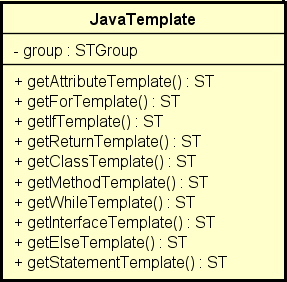
\includegraphics[scale=0.8,keepaspectratio]{img/server/JavaTemplate.png}}
\caption{\nogloxy{swedesigner::server::template::java::JavaTemplate}}
\end{figure}
\FloatBarrier
\begin{itemize}
\item \textbf{Descrizione}\\
questa classe è una implementazione di \texttt{Template} che permette di fornire un template di una classe, metodo o costrutto Java.
\item \textbf{Utilizzo}\\
viene utilizzata da \texttt{CompilerAssembler} che ritorna un' istanza di essa quando richiesto.
\item \textbf{Relazioni con altre classi}:
\begin{itemize}
\item \textit{OUT} \hyperref[\nogloxy{swedesigner::server::template::Template}]{\nogloxy{\texttt{Template}}}\\
questa interfaccia si occupa di fornire un oggetto template generico a chi lo richiede in modo da poter rendere estensibile il sistema aggiungendo un'implementazione concreta del template del linguaggio target desiderato.
\end{itemize}
\item \textbf{Attributi}:
\begin{itemize}
\item \nogloxy{\texttt{- group: STGroup}}
\\ Riferimento alla cartella da cui ricavare i file.st
\end{itemize}
\item \textbf{Metodi}:
\begin{itemize}
\item \nogloxy{\texttt{+  getMethodTemplate(): ST}}
\\ Ritorna il template per tradurre un oggetto ParsedMethod nel linguaggio Java.
\item \nogloxy{\texttt{+  getReturnTemplate(): ST}}
\\ Ritorna il template per tradurre un oggetto ParsedReturn nel linguaggio Java.
\item \nogloxy{\texttt{+ getAttributeTemplate(): ST}}
\\ Ritorna il template per tradurre un oggetto ParsedAttribute in linguaggio Java.
\item \nogloxy{\texttt{+ getClassTemplate(): ST}}
\\ Ritorna il template per tradurre un oggetto ParsedClass nel linguaggio Java.
\item \nogloxy{\texttt{+ getElseTemplate(): ST}}
\\ Ritorna il template per tradurre un oggetto ParsedElse nel linguaggio Java.
\item \nogloxy{\texttt{+ getForTemplate(): ST}}
\\ Ritorna il template per tradurre un oggetto ParsedFor nel linguaggio Java.
\item \nogloxy{\texttt{+ getIfTemplate(): ST}}
\\ Ritorna il template per tradurre un oggetto ParsedIf nel linguaggio Java.
\item \nogloxy{\texttt{+ getInterfaceTemplate(): ST}}
\\ Ritorna il template per tradurre un oggetto ParsedInterface nel linguaggio Java.
\item \nogloxy{\texttt{+ getStatementTemplate(): ST}}
\\ Ritorna il template per tradurre un oggetto ParsedStatement nel linguaggio Java.
\item \nogloxy{\texttt{+ getWhileTemplate(): ST}}
\\ Ritorna il template per tradurre un oggetto ParsedWhile nel linguaggio Java.
\end{itemize}
\end{itemize}
\subsection{\nogloxy{swedesigner::server::utility}}
\label{\nogloxy{swedesigner::server::utility}}
\subsubsection{Informazioni generali}
\begin{itemize}
\item \textbf{Descrizione}\\
Questo package contiene le componenti secondarie necessarie al server, indipendentemente dal linguaggio target dell'applicazione.
\item \textbf{Padre}: \hyperref[\nogloxy{swedesigner::server}]{\nogloxy{\texttt{server}}}
\end{itemize}
\subsubsection{Classi}
\subsubsubsection{\nogloxy{swedesigner::server::utility::Compressor}}
\label{\nogloxy{swedesigner::server::utility::Compressor}}
\begin{figure}[h]
\centering
\nogloxy{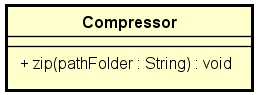
\includegraphics[scale=0.8,keepaspectratio]{img/server/Compressor.png}}
\caption{\nogloxy{swedesigner::server::utility::Compressor}}
\end{figure}
\FloatBarrier
\begin{itemize}
\item \textbf{Descrizione}\\
questa classe si occupa di creare e salvare su disco un archivio compresso contenente il progetto JSON, il codice sorgente e l'eseguibile generato che verrà poi messo a disposizione dell'utente che potrà scaricarlo.
\item \textbf{Utilizzo}\\
viene utilizzata da \texttt{RequestHandlerController} per creare l'archivio compresso dei file
\item \textbf{Relazioni con altre classi}:
\begin{itemize}
\item \textit{IN} \hyperref[\nogloxy{swedesigner::server::controller::RequestHandlerController}]{\nogloxy{\texttt{RequestHandlerController}}}\\
questa classe si occupa di ricevere le richieste REST provenienti dal client.
\end{itemize}
\item \textbf{Metodi}:
\begin{itemize}
\item \nogloxy{\texttt{+ zip(dirPath: String): void}}
\\ Crea una cartella zip contenente i file sorgenti e compilati del programma e la relativa stringa in formato .json.
\\ \textbf{Parametri}:
\begin{itemize}
\item \nogloxy{\texttt{dirPath: String}}
\\ Rappresenta la posizione della cartella, relativa ad una particolare richiesta, il cui contenuto verrà compresso in un file .zip.
\end{itemize}
\end{itemize}
\end{itemize}


\section{Tracciamento} \label{sec:tracc}
%%%%%%%%%%%%%%%%
%%  Tracciamento
%%%%%%%%%%%%%%%%



In questa sezione tracciamo le corrispondenze tra componenti dell'architettura (classi) e requisiti, cioè:
\begin{enumerate}
	\item per ogni componente, i requisiti che ne motivano l'esistenza;
	\item per ogni requisito, le componenti che servono a soddisfarlo.
\end{enumerate}



\subsection{Tracciamento Classi-Requisiti}
\normalsize
\begin{longtable}{|>{\centering}m{10cm}|m{3cm}<{\centering}|}
\hline 
\textbf{Classe} & \textbf{Requisiti}\\
\hline
\endhead
\hyperref[\nogloxy{swedesigner::client::model::celltypes::activity::ActivityDiagramElement}]{\nogloxy{\texttt{swedesigner::client::model::celltypes::-\linebreak activity::ActivityDiagramElement}}} & RFO4\\ \hline

\hyperref[\nogloxy{swedesigner::client::model::celltypes::activity::HxCustom}]{\nogloxy{\texttt{swedesigner::client::model::celltypes::-\linebreak activity::HxCustom}}} & RFO4.6\\ \hline

\hyperref[\nogloxy{swedesigner::client::model::celltypes::activity::HxElse}]{\nogloxy{\texttt{swedesigner::client::model::celltypes::-\linebreak activity::HxElse}}} & RFO4.3\\ \hline

\hyperref[\nogloxy{swedesigner::client::model::celltypes::activity::HxFor}]{\nogloxy{\texttt{swedesigner::client::model::celltypes::-\linebreak activity::HxFor}}} & RFO4.5\\ \hline

\hyperref[\nogloxy{swedesigner::client::model::celltypes::activity::HxIf}]{\nogloxy{\texttt{swedesigner::client::model::celltypes::-\linebreak activity::HxIf}}} & RFO4.2\\ \hline

\hyperref[\nogloxy{swedesigner::client::model::celltypes::activity::HxReturn}]{\nogloxy{\texttt{swedesigner::client::model::celltypes::-\linebreak activity::HxReturn}}} & RFO4.33\\ \hline

\hyperref[\nogloxy{swedesigner::client::model::celltypes::activity::HxVariable}]{\nogloxy{\texttt{swedesigner::client::model::celltypes::-\linebreak activity::HxVariable}}} & RFO4.1\\ \hline

\hyperref[\nogloxy{swedesigner::client::model::celltypes::activity::HxWhile}]{\nogloxy{\texttt{swedesigner::client::model::celltypes::-\linebreak activity::HxWhile}}} & RFO4.4\\ \hline

\hyperref[\nogloxy{swedesigner::client::model::celltypes::class::ClassDiagramElement}]{\nogloxy{\texttt{swedesigner::client::model::celltypes::-\linebreak class::ClassDiagramElement}}} & RFO3\\
& RFD3.8\\
& RFD3.9\\ \hline

\hyperref[\nogloxy{swedesigner::client::model::celltypes::class::ClassDiagramLink}]{\nogloxy{\texttt{swedesigner::client::model::celltypes::-\linebreak class::ClassDiagramLink}}} & RFO3\\
& RFO3.4\\ \hline

\hyperref[\nogloxy{swedesigner::client::model::celltypes::class::HxAssociation}]{\nogloxy{\texttt{swedesigner::client::model::celltypes::-\linebreak class::HxAssociation}}} & RFO3.5\\
& RFO3.5.1\\
& RFO3.5.2\\ \hline

\hyperref[\nogloxy{swedesigner::client::model::celltypes::class::HxClass}]{\nogloxy{\texttt{swedesigner::client::model::celltypes::-\linebreak class::HxClass}}} & RFO3.1\\ \hline

\hyperref[\nogloxy{swedesigner::client::model::celltypes::class::HxComment}]{\nogloxy{\texttt{swedesigner::client::model::celltypes::-\linebreak class::HxComment}}} & RFD3.8\\ \hline

\hyperref[\nogloxy{swedesigner::client::model::celltypes::class::HxGeneralization}]{\nogloxy{\texttt{swedesigner::client::model::celltypes::-\linebreak class::HxGeneralization}}} & RFO3.6\\ \hline

\hyperref[\nogloxy{swedesigner::client::model::celltypes::class::HxImplementation}]{\nogloxy{\texttt{swedesigner::client::model::celltypes::-\linebreak class::HxImplementation}}} & RFD3.7\\ \hline

\hyperref[\nogloxy{swedesigner::client::model::celltypes::class::HxInterface}]{\nogloxy{\texttt{swedesigner::client::model::celltypes::-\linebreak class::HxInterface}}} & RFO3.3\\ \hline

\hyperref[\nogloxy{swedesigner::client::model::celltypes::HxStereotype}]{\nogloxy{\texttt{swedesigner::client::model::celltypes::-\linebreak HxStereotype}}} & RFO3.2.6\\ \hline

\hyperref[\nogloxy{swedesigner::client::model::NewCellFactory}]{\nogloxy{\texttt{swedesigner::client::model::-\linebreak NewCellFactory}}} & RFO3.1\\
& RFO3.3\\
& RFO4.1\\
& RFO4.2\\
& RFO4.3\\
& RFO4.4\\
& RFO4.5\\
& RFO4.6\\ \hline

\hyperref[\nogloxy{swedesigner::client::model::NewCellModel}]{\nogloxy{\texttt{swedesigner::client::model::-\linebreak NewCellModel}}} & RFO3.1\\
& RFO3.3\\
& RFO4.1\\
& RFO4.2\\
& RFO4.3\\
& RFO4.4\\
& RFO4.5\\
& RFO4.6\\ \hline

\hyperref[\nogloxy{swedesigner::client::model::ProjectCommand}]{\nogloxy{\texttt{swedesigner::client::model::-\linebreak ProjectCommand}}} & RFO2\\
& RFO5\\
& RFO6\\ \hline

\hyperref[\nogloxy{swedesigner::client::model::ProjectModel}]{\nogloxy{\texttt{swedesigner::client::model::-\linebreak ProjectModel}}} & RFO1.1\\
& RFO3\\
& RFO4\\ \hline

\hyperref[\nogloxy{swedesigner::client::model::utility::ProjectStereotypes}]{\nogloxy{\texttt{swedesigner::client::model::utility::-\linebreak ProjectStereotypes}}} & RFO3.2.6\\ \hline

\hyperref[\nogloxy{swedesigner::client::view::AppView}]{\nogloxy{\texttt{swedesigner::client::view::AppView}}} & RFO1\\
& RFO2\\
& RFO3\\
& RFO4\\
& RFO5\\
& RFO6\\ \hline

\hyperref[\nogloxy{swedesigner::client::view::DetailsView}]{\nogloxy{\texttt{swedesigner::client::view::DetailsView}}} & RFO3.12\\
& RFO3.13\\
& RFO3.14\\
& RFO3.15\\
& RFO3.18\\
& RFO4.27\\
& RFO4.28\\
& RFO4.29\\
& RFO4.30\\
& RFO4.31\\
& RFO4.32\\
& RFO4.34\\ \hline

\hyperref[\nogloxy{swedesigner::client::view::NewCellView}]{\nogloxy{\texttt{swedesigner::client::view::NewCellView}}} & RFO3.1\\
& RFO3.3\\
& RFO4.1\\
& RFO4.2\\
& RFO4.3\\
& RFO4.4\\
& RFO4.5\\
& RFO4.6\\ \hline

\hyperref[\nogloxy{swedesigner::client::view::ProjectView}]{\nogloxy{\texttt{swedesigner::client::view::ProjectView}}} & RFO3\\
& RFO4\\ \hline

\hyperref[\nogloxy{swedesigner::server::Application}]{\nogloxy{\texttt{swedesigner::server::Application}}} & RFO8\\ \hline

\hyperref[\nogloxy{swedesigner::server::compiler::Compiler}]{\nogloxy{\texttt{swedesigner::server::compiler::-\linebreak Compiler}}} & RFO9\\ \hline

\hyperref[\nogloxy{swedesigner::server::compiler::java::JavaCompiler}]{\nogloxy{\texttt{swedesigner::server::compiler::java::-\linebreak JavaCompiler}}} & RFO9\\ \hline

\hyperref[\nogloxy{swedesigner::server::controller::RequestHandlerController}]{\nogloxy{\texttt{swedesigner::server::controller::-\linebreak RequestHandlerController}}} & RFO7\\
& RFO8\\
& RFO9\\
& RFO10\\
& RFO11\\ \hline

\hyperref[\nogloxy{swedesigner::server::generator::Generator}]{\nogloxy{\texttt{swedesigner::server::generator::-\linebreak Generator}}} & RFO8.2\\ \hline

\hyperref[\nogloxy{swedesigner::server::generator::java::JavaGenerator}]{\nogloxy{\texttt{swedesigner::server::generator::java::-\linebreak JavaGenerator}}} & RFO8.2\\ \hline

\hyperref[\nogloxy{swedesigner::server::parser::Parser}]{\nogloxy{\texttt{swedesigner::server::parser::Parser}}} & RFO8.1\\ \hline

\hyperref[\nogloxy{swedesigner::server::project::ParsedAttribute}]{\nogloxy{\texttt{swedesigner::server::project::-\linebreak ParsedAttribute}}} & RFO8.1\\ \hline

\hyperref[\nogloxy{swedesigner::server::project::ParsedClass}]{\nogloxy{\texttt{swedesigner::server::project::-\linebreak ParsedClass}}} & RFO8.1\\ \hline

\hyperref[\nogloxy{swedesigner::server::project::ParsedCustom}]{\nogloxy{\texttt{swedesigner::server::project::-\linebreak ParsedCustom}}} & RFO8.1\\ \hline

\hyperref[\nogloxy{swedesigner::server::project::ParsedElement}]{\nogloxy{\texttt{swedesigner::server::project::-\linebreak ParsedElement}}} & RFO8.1\\ \hline

\hyperref[\nogloxy{swedesigner::server::project::ParsedElse}]{\nogloxy{\texttt{swedesigner::server::project::-\linebreak ParsedElse}}} & RFO8.1\\ \hline

\hyperref[\nogloxy{swedesigner::server::project::ParsedException}]{\nogloxy{\texttt{swedesigner::server::project::-\linebreak ParsedException}}} & RFO6.1\\ \hline

\hyperref[\nogloxy{swedesigner::server::project::ParsedFor}]{\nogloxy{\texttt{swedesigner::server::project::-\linebreak ParsedFor}}} & RFO8.1\\ \hline

\hyperref[\nogloxy{swedesigner::server::project::ParsedIf}]{\nogloxy{\texttt{swedesigner::server::project::ParsedIf}}} & RFO8.1\\ \hline

\hyperref[\nogloxy{swedesigner::server::project::ParsedInstruction}]{\nogloxy{\texttt{swedesigner::server::project::-\linebreak ParsedInstruction}}} & RFO8.1\\ \hline

\hyperref[\nogloxy{swedesigner::server::project::ParsedInterface}]{\nogloxy{\texttt{swedesigner::server::project::-\linebreak ParsedInterface}}} & RFO8.1\\ \hline

\hyperref[\nogloxy{swedesigner::server::project::ParsedMethod}]{\nogloxy{\texttt{swedesigner::server::project::-\linebreak ParsedMethod}}} & RFO8.1\\ \hline

\hyperref[\nogloxy{swedesigner::server::project::ParsedProgram}]{\nogloxy{\texttt{swedesigner::server::project::-\linebreak ParsedProgram}}} & RFO8.1\\ \hline

\hyperref[\nogloxy{swedesigner::server::project::ParsedReturn}]{\nogloxy{\texttt{swedesigner::server::project::-\linebreak ParsedReturn}}} & RFO8.1\\ \hline

\hyperref[\nogloxy{swedesigner::server::project::ParsedStatement}]{\nogloxy{\texttt{swedesigner::server::project::-\linebreak ParsedStatement}}} & RFO8.1\\ \hline

\hyperref[\nogloxy{swedesigner::server::project::ParsedType}]{\nogloxy{\texttt{swedesigner::server::project::-\linebreak ParsedType}}} & RFO8.1\\ \hline

\hyperref[\nogloxy{swedesigner::server::project::ParsedWhile}]{\nogloxy{\texttt{swedesigner::server::project::-\linebreak ParsedWhile}}} & RFO8.1\\ \hline

\hyperref[\nogloxy{swedesigner::server::template::java::JavaTemplate}]{\nogloxy{\texttt{swedesigner::server::template::java::-\linebreak JavaTemplate}}} & RFO8.2\\ \hline

\hyperref[\nogloxy{swedesigner::server::template::Template}]{\nogloxy{\texttt{swedesigner::server::template::-\linebreak Template}}} & RFO8.2\\ \hline

\hyperref[\nogloxy{swedesigner::server::utility::Compressor}]{\nogloxy{\texttt{swedesigner::server::utility::-\linebreak Compressor}}} & RFO10\\ \hline

\caption[Tracciamento Classi-Requisiti]{Tracciamento Classi-Requisiti}
\label{tabella:class-requi}
\end{longtable}
\clearpage




\pagebreak

\subsection{Tracciamento Requisiti-Classi}
\normalsize
\begin{longtable}{|>{\centering}m{3cm}|m{10cm}<{\centering}|}
\hline 
\textbf{Requisito} & \textbf{Classi}\\
\hline
\endhead
RFO1 & \hyperref[\nogloxy{SWEDesigner::Client::Model::Utility::ProjectLoader}]{\nogloxy{\texttt{SWEDesigner::Client::Model::Utility::-\linebreak ProjectLoader}}}\\
& \hyperref[\nogloxy{SWEDesigner::Client::View::AppView}]{\nogloxy{\texttt{SWEDesigner::Client::View::AppView}}}\\ \hline

RFO1.1 & \hyperref[\nogloxy{SWEDesigner::Client::Model::ProjectModel}]{\nogloxy{\texttt{SWEDesigner::Client::Model::-\linebreak ProjectModel}}}\\ \hline

RFO2 & \hyperref[\nogloxy{SWEDesigner::Client::Model::ProjectCommand}]{\nogloxy{\texttt{SWEDesigner::Client::Model::-\linebreak ProjectCommand}}}\\
& \hyperref[\nogloxy{SWEDesigner::Client::Model::Utility::ProjectInitializer}]{\nogloxy{\texttt{SWEDesigner::Client::Model::Utility::-\linebreak ProjectInitializer}}}\\
& \hyperref[\nogloxy{SWEDesigner::Client::View::AppView}]{\nogloxy{\texttt{SWEDesigner::Client::View::AppView}}}\\ \hline

RFO3 & \hyperref[\nogloxy{SWEDesigner::Client::Collection::DiagramCollection}]{\nogloxy{\texttt{SWEDesigner::Client::Collection::-\linebreak DiagramCollection}}}\\
& \hyperref[\nogloxy{SWEDesigner::Client::Model::CellTypes::ClassDiagramElement}]{\nogloxy{\texttt{SWEDesigner::Client::Model::CellTypes::-\linebreak ClassDiagramElement}}}\\
& \hyperref[\nogloxy{SWEDesigner::Client::Model::ProjectModel}]{\nogloxy{\texttt{SWEDesigner::Client::Model::-\linebreak ProjectModel}}}\\
& \hyperref[\nogloxy{SWEDesigner::Client::View::AppView}]{\nogloxy{\texttt{SWEDesigner::Client::View::AppView}}}\\
& \hyperref[\nogloxy{SWEDesigner::Client::View::ProjectView}]{\nogloxy{\texttt{SWEDesigner::Client::View::ProjectView}}}\\ \hline

RFO3.1 & \hyperref[\nogloxy{SWEDesigner::Client::Model::CellTypes::HxAbstractClass}]{\nogloxy{\texttt{SWEDesigner::Client::Model::CellTypes::-\linebreak HxAbstractClass}}}\\
& \hyperref[\nogloxy{SWEDesigner::Client::Model::CellTypes::HxClass}]{\nogloxy{\texttt{SWEDesigner::Client::Model::CellTypes::-\linebreak HxClass}}}\\
& \hyperref[\nogloxy{SWEDesigner::Client::Model::CellTypes::HxInterface}]{\nogloxy{\texttt{SWEDesigner::Client::Model::CellTypes::-\linebreak HxInterface}}}\\
& \hyperref[\nogloxy{SWEDesigner::Client::Model::NewCellFactory}]{\nogloxy{\texttt{SWEDesigner::Client::Model::-\linebreak NewCellFactory}}}\\
& \hyperref[\nogloxy{SWEDesigner::Client::Model::NewCellModel}]{\nogloxy{\texttt{SWEDesigner::Client::Model::-\linebreak NewCellModel}}}\\
& \hyperref[\nogloxy{SWEDesigner::Client::View::DetailsView}]{\nogloxy{\texttt{SWEDesigner::Client::View::DetailsView}}}\\
& \hyperref[\nogloxy{SWEDesigner::Client::View::NewCellView}]{\nogloxy{\texttt{SWEDesigner::Client::View::NewCellView}}}\\ \hline

RFO3.1.3 & \hyperref[\nogloxy{SWEDesigner::Client::Model::CellTypes::HxStereotype}]{\nogloxy{\texttt{SWEDesigner::Client::Model::CellTypes::-\linebreak HxStereotype}}}\\
& \hyperref[\nogloxy{SWEDesigner::Client::Model::Utility::ProjectStereotypes}]{\nogloxy{\texttt{SWEDesigner::Client::Model::Utility::-\linebreak ProjectStereotypes}}}\\ \hline

RFO3.1.4.6.1 & \hyperref[\nogloxy{SWEDesigner::Client::View::DetailsView}]{\nogloxy{\texttt{SWEDesigner::Client::View::DetailsView}}}\\ \hline

RFO3.1.6.3.3.1 & \hyperref[\nogloxy{SWEDesigner::Client::View::DetailsView}]{\nogloxy{\texttt{SWEDesigner::Client::View::DetailsView}}}\\ \hline

RFO3.1.6.5.1 & \hyperref[\nogloxy{SWEDesigner::Client::View::DetailsView}]{\nogloxy{\texttt{SWEDesigner::Client::View::DetailsView}}}\\ \hline

RFO3.1.8.1 & \hyperref[\nogloxy{SWEDesigner::Client::View::DetailsView}]{\nogloxy{\texttt{SWEDesigner::Client::View::DetailsView}}}\\ \hline

RFO3.2 & \hyperref[\nogloxy{SWEDesigner::Client::Model::CellTypes::ClassDiagramLink}]{\nogloxy{\texttt{SWEDesigner::Client::Model::CellTypes::-\linebreak ClassDiagramLink}}}\\
& \hyperref[\nogloxy{SWEDesigner::Client::Model::CellTypes::GeneralizationCell}]{\nogloxy{\texttt{SWEDesigner::Client::Model::CellTypes::-\linebreak GeneralizationCell}}}\\
& \hyperref[\nogloxy{SWEDesigner::Client::Model::CellTypes::ImplementationCell}]{\nogloxy{\texttt{SWEDesigner::Client::Model::CellTypes::-\linebreak ImplementationCell}}}\\
& \hyperref[\nogloxy{SWEDesigner::Client::Model::NewCellFactory}]{\nogloxy{\texttt{SWEDesigner::Client::Model::-\linebreak NewCellFactory}}}\\
& \hyperref[\nogloxy{SWEDesigner::Client::Model::NewCellModel}]{\nogloxy{\texttt{SWEDesigner::Client::Model::-\linebreak NewCellModel}}}\\
& \hyperref[\nogloxy{SWEDesigner::Client::View::DetailsView}]{\nogloxy{\texttt{SWEDesigner::Client::View::DetailsView}}}\\
& \hyperref[\nogloxy{SWEDesigner::Client::View::NewCellView}]{\nogloxy{\texttt{SWEDesigner::Client::View::NewCellView}}}\\ \hline

RFO3.2.1 & \hyperref[\nogloxy{SWEDesigner::Client::Model::CellTypes::ClassDiagramLink}]{\nogloxy{\texttt{SWEDesigner::Client::Model::CellTypes::-\linebreak ClassDiagramLink}}}\\ \hline

RFO3.2.2 & \hyperref[\nogloxy{SWEDesigner::Client::Model::CellTypes::ClassDiagramLink}]{\nogloxy{\texttt{SWEDesigner::Client::Model::CellTypes::-\linebreak ClassDiagramLink}}}\\ \hline

RFO3.2.3 & \hyperref[\nogloxy{SWEDesigner::Client::Model::CellTypes::ClassDiagramLink}]{\nogloxy{\texttt{SWEDesigner::Client::Model::CellTypes::-\linebreak ClassDiagramLink}}}\\ \hline

RFO3.2.4 & \hyperref[\nogloxy{SWEDesigner::Client::Model::CellTypes::ClassDiagramLink}]{\nogloxy{\texttt{SWEDesigner::Client::Model::CellTypes::-\linebreak ClassDiagramLink}}}\\ \hline

RFO3.2.5 & \hyperref[\nogloxy{SWEDesigner::Client::Model::CellTypes::ClassDiagramLink}]{\nogloxy{\texttt{SWEDesigner::Client::Model::CellTypes::-\linebreak ClassDiagramLink}}}\\ \hline

RFO3.2.6 & \hyperref[\nogloxy{SWEDesigner::Client::Model::CellTypes::ClassDiagramLink}]{\nogloxy{\texttt{SWEDesigner::Client::Model::CellTypes::-\linebreak ClassDiagramLink}}}\\ \hline

RFO3.2.6.1 & \hyperref[\nogloxy{SWEDesigner::Client::View::DetailsView}]{\nogloxy{\texttt{SWEDesigner::Client::View::DetailsView}}}\\ \hline

RFO3.2.7 & \hyperref[\nogloxy{SWEDesigner::Client::Model::CellTypes::ClassDiagramLink}]{\nogloxy{\texttt{SWEDesigner::Client::Model::CellTypes::-\linebreak ClassDiagramLink}}}\\ \hline

RFO3.3 & \hyperref[\nogloxy{SWEDesigner::Client::Model::CellTypes::HxAnnotation}]{\nogloxy{\texttt{SWEDesigner::Client::Model::CellTypes::-\linebreak HxAnnotation}}}\\
& \hyperref[\nogloxy{SWEDesigner::Client::Model::NewCellFactory}]{\nogloxy{\texttt{SWEDesigner::Client::Model::-\linebreak NewCellFactory}}}\\
& \hyperref[\nogloxy{SWEDesigner::Client::Model::NewCellModel}]{\nogloxy{\texttt{SWEDesigner::Client::Model::-\linebreak NewCellModel}}}\\
& \hyperref[\nogloxy{SWEDesigner::Client::View::DetailsView}]{\nogloxy{\texttt{SWEDesigner::Client::View::DetailsView}}}\\
& \hyperref[\nogloxy{SWEDesigner::Client::View::NewCellView}]{\nogloxy{\texttt{SWEDesigner::Client::View::NewCellView}}}\\ \hline

RFO3.3.3.1 & \hyperref[\nogloxy{SWEDesigner::Client::View::DetailsView}]{\nogloxy{\texttt{SWEDesigner::Client::View::DetailsView}}}\\ \hline

RFO3.4 & \hyperref[\nogloxy{SWEDesigner::Client::Collection::DiagramCollection}]{\nogloxy{\texttt{SWEDesigner::Client::Collection::-\linebreak DiagramCollection}}}\\ \hline

RFO3.5 & \hyperref[\nogloxy{SWEDesigner::Client::Collection::DiagramCollection}]{\nogloxy{\texttt{SWEDesigner::Client::Collection::-\linebreak DiagramCollection}}}\\ \hline

RFO3.6 & \hyperref[\nogloxy{SWEDesigner::Client::Collection::DiagramCollection}]{\nogloxy{\texttt{SWEDesigner::Client::Collection::-\linebreak DiagramCollection}}}\\ \hline

RFD3.7 & \hyperref[\nogloxy{SWEDesigner::Client::Model::CellTypes::ClassDiagramElement}]{\nogloxy{\texttt{SWEDesigner::Client::Model::CellTypes::-\linebreak ClassDiagramElement}}}\\ \hline

RFD3.8 & \hyperref[\nogloxy{SWEDesigner::Client::Model::CellTypes::ClassDiagramElement}]{\nogloxy{\texttt{SWEDesigner::Client::Model::CellTypes::-\linebreak ClassDiagramElement}}}\\ \hline

RFD3.9 & \hyperref[\nogloxy{SWEDesigner::Client::Model::CellTypes::ClassDiagramElement}]{\nogloxy{\texttt{SWEDesigner::Client::Model::CellTypes::-\linebreak ClassDiagramElement}}}\\ \hline

RFD3.10 & \hyperref[\nogloxy{SWEDesigner::Client::Model::CellTypes::ClassDiagramElement}]{\nogloxy{\texttt{SWEDesigner::Client::Model::CellTypes::-\linebreak ClassDiagramElement}}}\\ \hline

RFO3.11 & \hyperref[\nogloxy{SWEDesigner::Client::View::DetailsView}]{\nogloxy{\texttt{SWEDesigner::Client::View::DetailsView}}}\\ \hline

RFO3.12 & \hyperref[\nogloxy{SWEDesigner::Client::View::DetailsView}]{\nogloxy{\texttt{SWEDesigner::Client::View::DetailsView}}}\\ \hline

RFO3.13 & \hyperref[\nogloxy{SWEDesigner::Client::View::DetailsView}]{\nogloxy{\texttt{SWEDesigner::Client::View::DetailsView}}}\\ \hline

RFO4 & \hyperref[\nogloxy{SWEDesigner::Client::Collection::DiagramCollection}]{\nogloxy{\texttt{SWEDesigner::Client::Collection::-\linebreak DiagramCollection}}}\\
& \hyperref[\nogloxy{SWEDesigner::Client::Model::CellTypes::ActivityDiagramElement}]{\nogloxy{\texttt{SWEDesigner::Client::Model::CellTypes::-\linebreak ActivityDiagramElement}}}\\
& \hyperref[\nogloxy{SWEDesigner::Client::Model::ProjectModel}]{\nogloxy{\texttt{SWEDesigner::Client::Model::-\linebreak ProjectModel}}}\\
& \hyperref[\nogloxy{SWEDesigner::Client::View::AppView}]{\nogloxy{\texttt{SWEDesigner::Client::View::AppView}}}\\
& \hyperref[\nogloxy{SWEDesigner::Client::View::ProjectView}]{\nogloxy{\texttt{SWEDesigner::Client::View::ProjectView}}}\\ \hline

RFO4.1 & \hyperref[\nogloxy{SWEDesigner::Client::Model::CellTypes::HxAssignment}]{\nogloxy{\texttt{SWEDesigner::Client::Model::CellTypes::-\linebreak HxAssignment}}}\\
& \hyperref[\nogloxy{SWEDesigner::Client::Model::CellTypes::HxInitialization}]{\nogloxy{\texttt{SWEDesigner::Client::Model::CellTypes::-\linebreak HxInitialization}}}\\
& \hyperref[\nogloxy{SWEDesigner::Client::Model::NewCellFactory}]{\nogloxy{\texttt{SWEDesigner::Client::Model::-\linebreak NewCellFactory}}}\\
& \hyperref[\nogloxy{SWEDesigner::Client::Model::NewCellModel}]{\nogloxy{\texttt{SWEDesigner::Client::Model::-\linebreak NewCellModel}}}\\
& \hyperref[\nogloxy{SWEDesigner::Client::View::DetailsView}]{\nogloxy{\texttt{SWEDesigner::Client::View::DetailsView}}}\\
& \hyperref[\nogloxy{SWEDesigner::Client::View::NewCellView}]{\nogloxy{\texttt{SWEDesigner::Client::View::NewCellView}}}\\ \hline

RFO4.1.4.1 & \hyperref[\nogloxy{SWEDesigner::Client::View::DetailsView}]{\nogloxy{\texttt{SWEDesigner::Client::View::DetailsView}}}\\ \hline

RFO4.2 & \hyperref[\nogloxy{SWEDesigner::Client::Model::NewCellFactory}]{\nogloxy{\texttt{SWEDesigner::Client::Model::-\linebreak NewCellFactory}}}\\
& \hyperref[\nogloxy{SWEDesigner::Client::Model::NewCellModel}]{\nogloxy{\texttt{SWEDesigner::Client::Model::-\linebreak NewCellModel}}}\\
& \hyperref[\nogloxy{SWEDesigner::Client::View::DetailsView}]{\nogloxy{\texttt{SWEDesigner::Client::View::DetailsView}}}\\
& \hyperref[\nogloxy{SWEDesigner::Client::View::NewCellView}]{\nogloxy{\texttt{SWEDesigner::Client::View::NewCellView}}}\\ \hline

RFO4.2.3.1 & \hyperref[\nogloxy{SWEDesigner::Client::View::DetailsView}]{\nogloxy{\texttt{SWEDesigner::Client::View::DetailsView}}}\\ \hline

RFO4.3 & \hyperref[\nogloxy{SWEDesigner::Client::Model::CellTypes::HxIf}]{\nogloxy{\texttt{SWEDesigner::Client::Model::CellTypes::-\linebreak HxIf}}}\\
& \hyperref[\nogloxy{SWEDesigner::Client::Model::NewCellFactory}]{\nogloxy{\texttt{SWEDesigner::Client::Model::-\linebreak NewCellFactory}}}\\
& \hyperref[\nogloxy{SWEDesigner::Client::Model::NewCellModel}]{\nogloxy{\texttt{SWEDesigner::Client::Model::-\linebreak NewCellModel}}}\\
& \hyperref[\nogloxy{SWEDesigner::Client::View::DetailsView}]{\nogloxy{\texttt{SWEDesigner::Client::View::DetailsView}}}\\
& \hyperref[\nogloxy{SWEDesigner::Client::View::NewCellView}]{\nogloxy{\texttt{SWEDesigner::Client::View::NewCellView}}}\\ \hline

RFO4.3.5.1 & \hyperref[\nogloxy{SWEDesigner::Client::View::DetailsView}]{\nogloxy{\texttt{SWEDesigner::Client::View::DetailsView}}}\\ \hline

RFO4.4 & \hyperref[\nogloxy{SWEDesigner::Client::Model::CellTypes::HxWhile}]{\nogloxy{\texttt{SWEDesigner::Client::Model::CellTypes::-\linebreak HxWhile}}}\\
& \hyperref[\nogloxy{SWEDesigner::Client::Model::NewCellFactory}]{\nogloxy{\texttt{SWEDesigner::Client::Model::-\linebreak NewCellFactory}}}\\
& \hyperref[\nogloxy{SWEDesigner::Client::Model::NewCellModel}]{\nogloxy{\texttt{SWEDesigner::Client::Model::-\linebreak NewCellModel}}}\\
& \hyperref[\nogloxy{SWEDesigner::Client::View::DetailsView}]{\nogloxy{\texttt{SWEDesigner::Client::View::DetailsView}}}\\
& \hyperref[\nogloxy{SWEDesigner::Client::View::NewCellView}]{\nogloxy{\texttt{SWEDesigner::Client::View::NewCellView}}}\\ \hline

RFO4.4.4.1 & \hyperref[\nogloxy{SWEDesigner::Client::View::DetailsView}]{\nogloxy{\texttt{SWEDesigner::Client::View::DetailsView}}}\\ \hline

RFO4.5 & \hyperref[\nogloxy{SWEDesigner::Client::Model::CellTypes::HxFor}]{\nogloxy{\texttt{SWEDesigner::Client::Model::CellTypes::-\linebreak HxFor}}}\\
& \hyperref[\nogloxy{SWEDesigner::Client::Model::NewCellFactory}]{\nogloxy{\texttt{SWEDesigner::Client::Model::-\linebreak NewCellFactory}}}\\
& \hyperref[\nogloxy{SWEDesigner::Client::Model::NewCellModel}]{\nogloxy{\texttt{SWEDesigner::Client::Model::-\linebreak NewCellModel}}}\\
& \hyperref[\nogloxy{SWEDesigner::Client::View::DetailsView}]{\nogloxy{\texttt{SWEDesigner::Client::View::DetailsView}}}\\
& \hyperref[\nogloxy{SWEDesigner::Client::View::NewCellView}]{\nogloxy{\texttt{SWEDesigner::Client::View::NewCellView}}}\\ \hline

RFO4.5.6.1 & \hyperref[\nogloxy{SWEDesigner::Client::View::DetailsView}]{\nogloxy{\texttt{SWEDesigner::Client::View::DetailsView}}}\\ \hline

RFO4.6 & \hyperref[\nogloxy{SWEDesigner::Client::Model::CellTypes::HxCustom}]{\nogloxy{\texttt{SWEDesigner::Client::Model::CellTypes::-\linebreak HxCustom}}}\\
& \hyperref[\nogloxy{SWEDesigner::Client::Model::NewCellFactory}]{\nogloxy{\texttt{SWEDesigner::Client::Model::-\linebreak NewCellFactory}}}\\
& \hyperref[\nogloxy{SWEDesigner::Client::Model::NewCellModel}]{\nogloxy{\texttt{SWEDesigner::Client::Model::-\linebreak NewCellModel}}}\\
& \hyperref[\nogloxy{SWEDesigner::Client::View::DetailsView}]{\nogloxy{\texttt{SWEDesigner::Client::View::DetailsView}}}\\
& \hyperref[\nogloxy{SWEDesigner::Client::View::NewCellView}]{\nogloxy{\texttt{SWEDesigner::Client::View::NewCellView}}}\\ \hline

RFO4.20 & \hyperref[\nogloxy{SWEDesigner::Client::View::DetailsView}]{\nogloxy{\texttt{SWEDesigner::Client::View::DetailsView}}}\\ \hline

RFO4.21 & \hyperref[\nogloxy{SWEDesigner::Client::View::DetailsView}]{\nogloxy{\texttt{SWEDesigner::Client::View::DetailsView}}}\\ \hline

RFO4.22 & \hyperref[\nogloxy{SWEDesigner::Client::View::DetailsView}]{\nogloxy{\texttt{SWEDesigner::Client::View::DetailsView}}}\\ \hline

RFO4.23 & \hyperref[\nogloxy{SWEDesigner::Client::View::DetailsView}]{\nogloxy{\texttt{SWEDesigner::Client::View::DetailsView}}}\\ \hline

RFO4.24 & \hyperref[\nogloxy{SWEDesigner::Client::View::DetailsView}]{\nogloxy{\texttt{SWEDesigner::Client::View::DetailsView}}}\\ \hline

RFO4.25 & \hyperref[\nogloxy{SWEDesigner::Client::View::DetailsView}]{\nogloxy{\texttt{SWEDesigner::Client::View::DetailsView}}}\\ \hline

RFO4.26 & \hyperref[\nogloxy{SWEDesigner::Client::Model::CellTypes::HxReturn}]{\nogloxy{\texttt{SWEDesigner::Client::Model::CellTypes::-\linebreak HxReturn}}}\\
& \hyperref[\nogloxy{SWEDesigner::Client::View::NewCellView}]{\nogloxy{\texttt{SWEDesigner::Client::View::NewCellView}}}\\ \hline

RFO5 & \hyperref[\nogloxy{SWEDesigner::Client::Model::ProjectCommand}]{\nogloxy{\texttt{SWEDesigner::Client::Model::-\linebreak ProjectCommand}}}\\
& \hyperref[\nogloxy{SWEDesigner::Client::Model::Utility::ProjectSaver}]{\nogloxy{\texttt{SWEDesigner::Client::Model::Utility::-\linebreak ProjectSaver}}}\\
& \hyperref[\nogloxy{SWEDesigner::Client::View::AppView}]{\nogloxy{\texttt{SWEDesigner::Client::View::AppView}}}\\ \hline

RFO6 & \hyperref[\nogloxy{SWEDesigner::Client::Model::ProjectCommand}]{\nogloxy{\texttt{SWEDesigner::Client::Model::-\linebreak ProjectCommand}}}\\
& \hyperref[\nogloxy{SWEDesigner::Client::Model::Utility::ProjectGenerator}]{\nogloxy{\texttt{SWEDesigner::Client::Model::Utility::-\linebreak ProjectGenerator}}}\\
& \hyperref[\nogloxy{SWEDesigner::Client::View::AppView}]{\nogloxy{\texttt{SWEDesigner::Client::View::AppView}}}\\ \hline

RFO7 & \hyperref[\nogloxy{SWEDesigner::Server::Controller::RequestHandlerController}]{\nogloxy{\texttt{SWEDesigner::Server::Controller::-\linebreak RequestHandlerController}}}\\ \hline

RFO8 & \hyperref[\nogloxy{SWEDesigner::Server::Controller::RequestHandlerController}]{\nogloxy{\texttt{SWEDesigner::Server::Controller::-\linebreak RequestHandlerController}}}\\ \hline

RFO8.1 & \hyperref[\nogloxy{SWEDesigner::Server::Parser::Parser}]{\nogloxy{\texttt{SWEDesigner::Server::Parser::Parser}}}\\
& \hyperref[\nogloxy{SWEDesigner::Server::Project::ParsedAssignment}]{\nogloxy{\texttt{SWEDesigner::Server::Project::-\linebreak ParsedAssignment}}}\\
& \hyperref[\nogloxy{SWEDesigner::Server::Project::ParsedAttribute}]{\nogloxy{\texttt{SWEDesigner::Server::Project::-\linebreak ParsedAttribute}}}\\
& \hyperref[\nogloxy{SWEDesigner::Server::Project::ParsedClass}]{\nogloxy{\texttt{SWEDesigner::Server::Project::-\linebreak ParsedClass}}}\\
& \hyperref[\nogloxy{SWEDesigner::Server::Project::ParsedCustom}]{\nogloxy{\texttt{SWEDesigner::Server::Project::-\linebreak ParsedCustom}}}\\
& \hyperref[\nogloxy{SWEDesigner::Server::Project::ParsedElement}]{\nogloxy{\texttt{SWEDesigner::Server::Project::-\linebreak ParsedElement}}}\\
& \hyperref[\nogloxy{SWEDesigner::Server::Project::ParsedFor}]{\nogloxy{\texttt{SWEDesigner::Server::Project::-\linebreak ParsedFor}}}\\
& \hyperref[\nogloxy{SWEDesigner::Server::Project::ParsedIf}]{\nogloxy{\texttt{SWEDesigner::Server::Project::ParsedIf}}}\\
& \hyperref[\nogloxy{SWEDesigner::Server::Project::ParsedInitialize}]{\nogloxy{\texttt{SWEDesigner::Server::Project::-\linebreak ParsedInitialize}}}\\
& \hyperref[\nogloxy{SWEDesigner::Server::Project::ParsedInstruction}]{\nogloxy{\texttt{SWEDesigner::Server::Project::-\linebreak ParsedInstruction}}}\\
& \hyperref[\nogloxy{SWEDesigner::Server::Project::ParsedInterface}]{\nogloxy{\texttt{SWEDesigner::Server::Project::-\linebreak ParsedInterface}}}\\
& \hyperref[\nogloxy{SWEDesigner::Server::Project::ParsedMethod}]{\nogloxy{\texttt{SWEDesigner::Server::Project::-\linebreak ParsedMethod}}}\\
& \hyperref[\nogloxy{SWEDesigner::Server::Project::ParsedProgram}]{\nogloxy{\texttt{SWEDesigner::Server::Project::-\linebreak ParsedProgram}}}\\
& \hyperref[\nogloxy{SWEDesigner::Server::Project::ParsedReturn}]{\nogloxy{\texttt{SWEDesigner::Server::Project::-\linebreak ParsedReturn}}}\\
& \hyperref[\nogloxy{SWEDesigner::Server::Project::ParsedType}]{\nogloxy{\texttt{SWEDesigner::Server::Project::-\linebreak ParsedType}}}\\
& \hyperref[\nogloxy{SWEDesigner::Server::Project::ParsedWhile}]{\nogloxy{\texttt{SWEDesigner::Server::Project::-\linebreak ParsedWhile}}}\\ \hline

RFO8.2 & \hyperref[\nogloxy{SWEDesigner::Server::Generator::Generator}]{\nogloxy{\texttt{SWEDesigner::Server::Generator::-\linebreak Generator}}}\\
& \hyperref[\nogloxy{SWEDesigner::Server::Generator::GeneratorAssembler}]{\nogloxy{\texttt{SWEDesigner::Server::Generator::-\linebreak GeneratorAssembler}}}\\
& \hyperref[\nogloxy{SWEDesigner::Server::Generator::Java::JavaGenerator}]{\nogloxy{\texttt{SWEDesigner::Server::Generator::Java::-\linebreak JavaGenerator}}}\\
& \hyperref[\nogloxy{SWEDesigner::Server::Template::Java::JavaTemplate}]{\nogloxy{\texttt{SWEDesigner::Server::Template::Java::-\linebreak JavaTemplate}}}\\
& \hyperref[\nogloxy{SWEDesigner::Server::Template::Template}]{\nogloxy{\texttt{SWEDesigner::Server::Template::-\linebreak Template}}}\\
& \hyperref[\nogloxy{SWEDesigner::Server::Template::TemplateAssembler}]{\nogloxy{\texttt{SWEDesigner::Server::Template::-\linebreak TemplateAssembler}}}\\ \hline

RFO9 & \hyperref[\nogloxy{SWEDesigner::Server::Compiler::Compiler}]{\nogloxy{\texttt{SWEDesigner::Server::Compiler::-\linebreak Compiler}}}\\
& \hyperref[\nogloxy{SWEDesigner::Server::Compiler::CompilerAssembler}]{\nogloxy{\texttt{SWEDesigner::Server::Compiler::-\linebreak CompilerAssembler}}}\\
& \hyperref[\nogloxy{SWEDesigner::Server::Compiler::Java::JavaCompiler}]{\nogloxy{\texttt{SWEDesigner::Server::Compiler::Java::-\linebreak JavaCompiler}}}\\
& \hyperref[\nogloxy{SWEDesigner::Server::Controller::RequestHandlerController}]{\nogloxy{\texttt{SWEDesigner::Server::Controller::-\linebreak RequestHandlerController}}}\\ \hline

RFO10 & \hyperref[\nogloxy{SWEDesigner::Server::Controller::RequestHandlerController}]{\nogloxy{\texttt{SWEDesigner::Server::Controller::-\linebreak RequestHandlerController}}}\\
& \hyperref[\nogloxy{SWEDesigner::Server::Utility::Compressor}]{\nogloxy{\texttt{SWEDesigner::Server::Utility::-\linebreak Compressor}}}\\ \hline

RFO11 & \hyperref[\nogloxy{SWEDesigner::Server::Controller::RequestHandlerController}]{\nogloxy{\texttt{SWEDesigner::Server::Controller::-\linebreak RequestHandlerController}}}\\ \hline

\caption[Tracciamento Requisiti-Classi]{Tracciamento Requisiti-Classi}
\label{tabella:requi-class}
\end{longtable}
\clearpage



\end{document}
